\documentclass[12pt, a4paper]{report}
\usepackage[italian]{babel}
\usepackage[utf8]{inputenc}
\usepackage{amsmath, amsfonts, amssymb, amsthm}
\usepackage{graphicx, appendix, geometry}
\geometry{a4paper, top=2cm, bottom=3cm, left=2cm, right=2cm, bindingoffset=5mm}

\author{Athos Innocenti}
\title{\Huge Elettronica}\date{}\author{}
\begin{document}
\maketitle
\tableofcontents

\chapter{Semiconduttori e Diodi}
I \textbf{semiconduttori} sono materiali parzialmente conduttori cioè hanno una conducibilità più alta degli \textit{isolanti} (materiali \textit{dielettrici} in cui gli elettroni sono fissi in un reticolo quindi sono incapaci di muoversi e per questo non scorre corrente), ma minore dei \textit{conduttori} (tutti i \textit{metalli} nei quali, se si applica un potenziale, scorre corrente perché ci sono elettroni liberi disponibili all'interno del materiale). Tendenzialmente i semiconduttori sono degli isolanti, ma sotto opportune condizioni si comportano come conduttori. In questi materiali gli atomi sono legati tra loro tramite legami \textbf{covalenti} come nel caso dei materiali isolanti, con i quali condividono anche la dipendenza della conducibilità dalla \textit{temperatura}.
\begin{figure}[h]
\centering
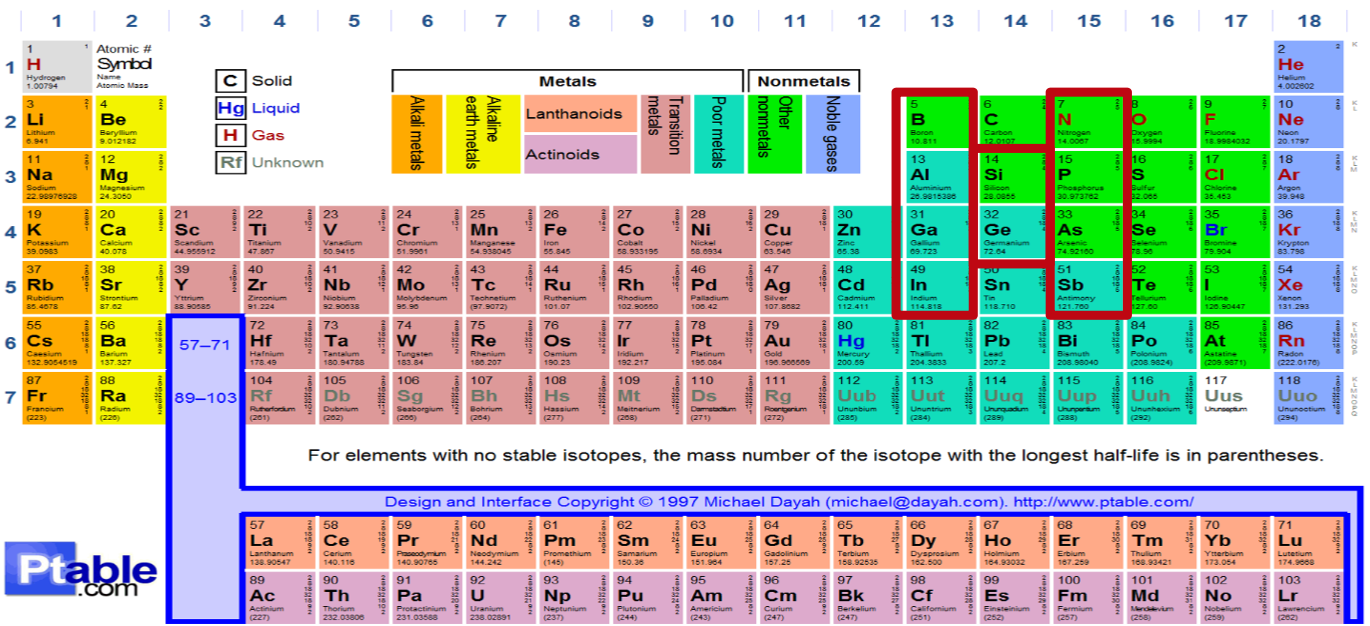
\includegraphics[scale=0.4,angle=0]{tavola_periodica.png}
\caption{Tavola periodica}
\end{figure}

I più comuni semiconduttori sono il \textbf{silicio} e il \textbf{germanio} che, trovandosi nella $IV^{a}$ colonna della tavola periodica, hanno quattro elettroni nell'orbitale più esterno. Sono gli unici semiconduttori \textbf{non composti}, cioè costituiti da atomi di un solo tipo. Altri possibili semiconduttori sono i seguenti composti \textbf{binari}: arseniuro di gallio GaAs, nitruro di gallio GaN, fosfuro di indio InP e il carburo di silicio SiC (un composto 4\,-\,4 perché sia il carbonio che il silicio appartengono alla quarta colonna), tutti formati da un elemento della $III^{a}$ colonna e da uno della $V^{a}$ e per questo si comportano come un elemento della quarta colonna (perché in media hanno quattro elettroni).\\Dunque, nei semiconduttori gli atomi coinvolti sono tutti collocati a cavallo della $IV^{a}$ colonna della tavola periodica: quella del carbonio (ma da solo non è usato come semiconduttore), silicio e germanio che hanno orbitali mezzi pieni e mezzi vuoti; cioè ci sono quattro elettroni e quattro spazi vuoti.

Di base, un materiale semiconduttore da solo è un materiale debolmente o per niente conduttore e non esprime, da solo, nessuna particolare proprietà, tuttavia diventa un materiale utilizzabile nel campo dell'elettronica quando viene \textbf{drogato}. Durante questo processo si parte da una matrice cristallina di materiale base che deve essere un materiale della quarta colonna, per esempio il silicio, e per \textbf{diffusione} si inserisce al suo interno una piccola quantità (circa una parte per miliardo) di \textbf{impurità}, ovvero di materiali appartenenti alla $III^{a}$ o alla $V^{a}$ colonna; generalmente sono rispettivamente il boro \textbf{B} e il fosforo \textbf{P}.

Nel caso del fosforo si parla di \textbf{impurità di quinta colonna} caratterizzata dall'avere un \textit{eccesso} di elettroni perché il fosforo ne ha cinque rispetto ai quattro del silicio. Il fosforo, inserito nella matrice di silicio, fornisce degli elettroni aggiuntivi (rappresentati tramite una carica negativa) rispetto al \textit{reticolo di base}, la struttura della matrice rimane la stessa, ovvero il reticolo del silicio, ma di tanto in tanto ci sono degli elettroni in più che rendono il materiale più \textbf{elettronegativo}, cioè più disponibile a fornire degli elettroni, e quindi si guadagna una certa conducibilità elettrica. In generale, quando si aggiunge un materiale \textit{drogante} di quinta colonna, il materiale che si ottiene è detto di \textbf{tipo n}. Quindi se il materiale di base è drogato da una impurità di tipo n significa che c'è un eccesso di elettroni, cioè di cariche negativa all'interno del materiale.

Nel caso del boro, o più in generale di un drogante di terza colonna, si parla di \textbf{impurità di terza colonna} caratterizzata dall'avere un \textit{difetto} di elettroni perché l'elemento di terza colonna ha solo tre elettroni rispetto ai quattro del reticolo. A livello pratico è come se per ogni impurità nella matrice si avesse un piccolo buco, cioè una mancanza di elettrone che prende il nome di \textbf{lacuna} e in genere si modella come se fosse una \textit{carica positiva}, infatti matematicamente le lacune vengono trattate come se fossero delle vere cariche positive per far tornare correttamente i conti. Il materiale ottenuto tramite questo secondo tipo di impurità è detto di \textbf{tipo p}.

Nell'interazione tra un materiale di tipo p e un materiale di tipo n si nota che gli elettroni in eccesso nel materiale di tipo n passano attraverso le lacune del materiale di tipo p.

Il drogaggio in entrambi i casi può essere fatto sia utilizzando un materiale \textbf{puro} come il silicio e il germanio, oppure tramite un materiale \textbf{composto}, l'importante è che il materiale sia mediamente di quarta colonna. Il silicio è di gran lunga il materiale più usato però non è strettamente quello che ma prestazioni migliori, il germanio viene maggiormente utilizzato per i dispositivi a radiofrequenza ma è molto più raro come lo sono anche GaAs, GaN e InP. SiC è costituito da carbonio e silicio che sono facilmente reperibili ma deve essere costruito quindi rimane comunque mediamente costoso.\\Lo specifico materiale da utilizzare dipende dall'elettronica che si deve andare a costruire. Per l'elettronica digitale, come celle logiche e microprocessori, si può utilizzare la tecnologia del silicio più i vari droganti. Per l'elettronica di potenza ad alte prestazioni si tende a preferire il nitruro di gallio o il carburo di silicio per le loro caratteristiche. Per i dispositivi optoelettronici, per esempio i LED, si usano invece il fosfuro di indio e l'arseniuro di gallio.

\section{Giunzioni PN}
Si ottengono quando si fa un drogaggio del silicio, cioè quando si aggiunge un materiale al silicio puro. L'aspetto particolare non è tanto il drogaggio del materiale di base quanto il mettere in contatto materiali drogati di tipo diverso, p ed n.

Nel caso dei materiali di tipo p si va a studiare il numero di \textbf{accettori}, indicato con $N_{a}$, rappresentante il numero di \textit{lacune} per unità di volume. Al contrario, per i materiali di tipo n si va a studiare il numero $N_{d}$ rappresentante il numero di \textbf{donatori} per unità di volume, cioè il numero di atomi che donano un elettrone. Sia $N_{a}$ che $N_{d}$ sono dell'ordine di $10^{-9}\,, 10^{-10}$ cioè un atomo ogni $10^{10}$ circa è un drogante di tipo p o n.

Più il silicio di base viene drogato e più esso tenderà a diventare un materiale con un comportamento sempre più lontano da quello del silicio di base. Di base il silicio si organizza in una \textit{matrice cristallina}, cioè come un \textit{cristallo} che non lascia passare lacune ed elettroni ma aggiungendo delle impurità si rendendo disponibili elettroni in più oppure delle lacune in cui potranno finire degli elettroni.

Per ottenere le \textbf{giunzioni p\,-\,n} si parte da una matrice di silicio la quale, tramite un processo di diffusione dall'alto, viene prima drogata con un drogante di tipo n andando a creare una \textit{tasca} e poi su una certa sezione già drogata della tasca viene ulteriormente inserito un drogante di tipo p (la diffusione può essere effettuata selettivamente in specifiche aree della matrice in base alle esigenze). La giunzione pn si formerà quindi lungo il \textit{bordo di confine} tra il drogaggio di tipo p e quello di tipo n.
\begin{figure}[ht]
\centering
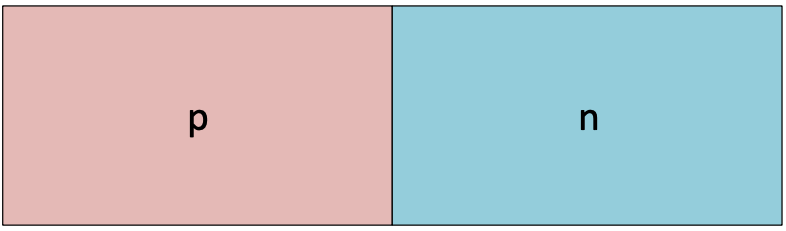
\includegraphics[scale=0.4,angle=0]{giunzione_pn.png}
\caption{Giunzione PN}
\end{figure}

Preso un materiale di tipo p avente un eccesso di lacune rispetto al reticolo e uno di tipo n con un eccesso di elettroni, nonostante le impurità i due materiali sono entrambi \textit{elettricamente neutri}. Lo sbilanciamento di elettroni in un lato e di lacune disponibili nell'altro fa sì che nel momento in cui un materiale di tipo p e uno di tipo n entrano in contatto si verifica un fenomeno di \textbf{migrazione} per cui statisticamente gli elettroni in eccesso nel materiale di tipo n tendono a migrare nel materiale di tipo p avente dello spazio libero dato dalle lacune.
\begin{figure}[h]
\centering
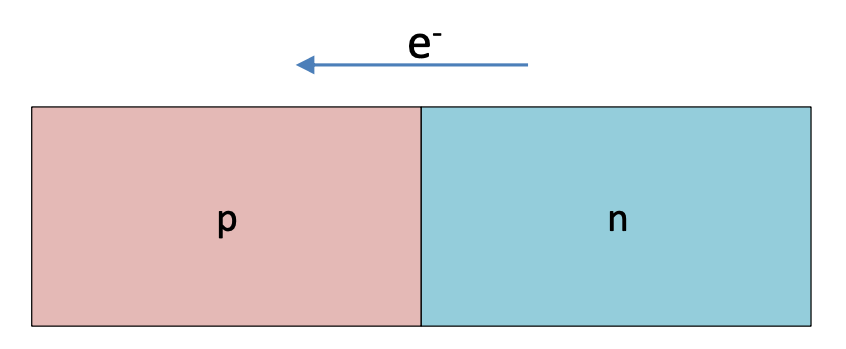
\includegraphics[scale=0.4,angle=0]{giunzione_pn_elettroni.png}
\caption{Migrazione degli elettroni}
\end{figure}

Via via che gli elettroni passano nel materiale di tipo p ognuno di essi si inserisce in una lacuna, riempiendola. Nel far ciò il materiale di tipo p passa dall'essere un materiale neutro (era un materiale della terza colonna con tre protoni e tre elettroni) ad essere \textit{negativamente carico} e questo comporta che la carica negativa che si è venuta a creare emette un \textbf{campo elettrico} che respinge altre cariche negative. Per cui, via via che gli elettroni passano nel materiale di tipo p tale materiale diventa più carico negativamente e si genera un campo elettrico negativo, inoltre gli elettroni che sono passati hanno liberato posti all'interno del materiale di tipo n nel quale quindi si crea una \textit{carica positiva}. Si arriva quindi ad un punto in cui sono passati un certo numero di elettroni che hanno generato un campo elettrico che impedisce ad altri elettroni nel materiale di tipo n di passare, si ha un \textbf{equilibrio}.

All'equilibrio, un certo numero di elettroni è passato nel materiale di tipo p e ha creato una zona a carica nettamente negativa e si sono formate un certo numero di lacune nel materiale di tipo n che hanno creato una zona a carica nettamente positiva. In queste condizioni, non è possibile far fluire ulteriori elettroni perché verrebbero respinti dal campo elettrico generato dagli elettroni passati in precedenza.
\begin{figure}[ht]
\centering
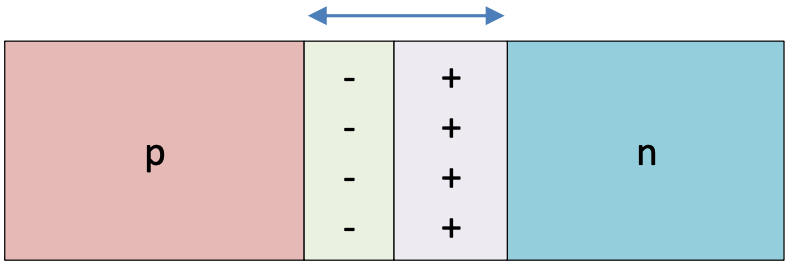
\includegraphics[scale=0.4,angle=0]{giunzione_pn_equilibrio.png}
\caption{Giunzione PN all'equilibrio}
\end{figure}

Nella zona a carica negativa non c'è più spazio per poter far arrivare e ospitare ulteriori elettroni e, analogamente, nella zona a carica positiva sono presenti tutti quegli atomi che in precedenza avevano cinque elettroni e ora ne hanno quattro, quindi non si possono più spostare altri elettroni perché si è tornati alla conformazione del reticolo cristallino del silicio con quattro elettroni; è silicio carico positivamente ma non ha elettroni trasferibili. Questo sbilanciamento di carica (da un lato una carica negativa netta e dall'altro una carica positiva netta) come già detto provoca un campo elettrico che blocca l'ulteriore diffusione di elettroni e la regione in cui sono presenti le due cariche nette opposte è chiamata \textbf{regione di svuotamento} o \textbf{regione di carica spaziale}. Di svuotamento nel senso che in quella regione sono stati eliminati tutti i \textit{portatori} di carica; di carica spaziale nel senso che questo procedimento ha portato a creare una \textit{densità di carica} positiva e negativa che implica la formazione di un campo elettrico.
\begin{figure}[h]
\centering
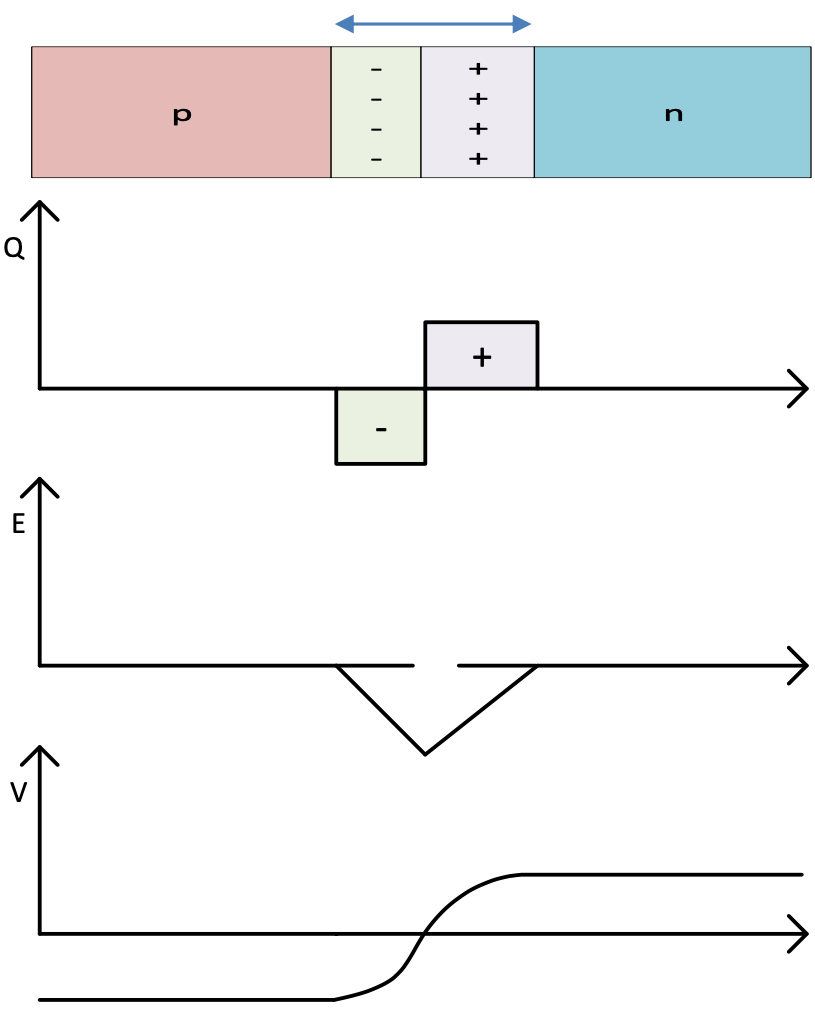
\includegraphics[scale=0.45,angle=0]{giunzione_pn_grafici.png}
\caption{Cariche, campo elettrico e potenziale della giunzione PN}
\label{grafici}
\end{figure}

Come si nota in figura \ref{grafici}, nel dominio della carica nella ragione di svuotamento relativa alla zona p si crea una regione di cariche nettamente negative mentre in quella relativa alla zona n se ne crea una di cariche nettamente positiva.

Dallo studio della carica è possibile ricavare informazioni relative sia al campo elettrico che al potenziale. Percorrendo l'asse \textit{x} da sinistra verso destra e integrando rispetto alle cariche incontrate, cioè integrando la \textit{distribuzione} di carica (la funzione rappresentata nel primo grafico - per semplicità si è presa esattamente rettangolare cioè una distribuzione uniforme), si ricava il campo elettrico $E(x) = \int q\,dx$ (secondo grafico di figura \ref{grafici}) che è una funzione decrescente nell'intervallo in cui ci sono solo cariche negative, ha il minimo in corrispondenza della giunzione pn e da lì diventa una funzione crescente dal momento in cui si entra nella zona con carica positiva netta. Sia la crescita che la decrescita sono entrambe \textit{lineari} avendo supposto una distribuzione uniforme in entrambe le zone. Inoltre la funzione $E(x)$ nei due estremi vale $0$ perché la quantità di carica positiva e negativa è \textit{la stessa} e questo è dovuto al fatto che ad ogni elettrone passato corrisponde una lacuna lasciata.

L'\textit{estensione} della zona a carica positiva e di quella a carica negativa non sono uguali perché l'estensione fisica della regione di svuotamento sia nel lato p che nel lato n è \textit{direttamente proporzionale} a quante lacune e a quanti elettroni ci sono per unità di volume. Si scambia la stessa quantità di elettroni e lacune ma la dimensione delle due zone dipende dalla quantità di portatori, cioè dipende dalla \textit{densità} del drogante. Se per esempio si suppone che il drogaggio della parte p sia il doppio di quello della parte n (quindi $N_{a} > N_{d}$), siccome il numero totale di elettroni è lo stesso a destra e a sinistra, una volta riempita tutta la regione di svuotamento si sa che ci sono $N_{a}$ elettroni per unità di volume nella zona costituente la carica negativa netta. Posta $x_p$ la lunghezza della zona a carica negativa netta e $x_{n}$ quella della zona a carica positiva netta, $N_{a} \cdot x_{p}$ rappresenta la quantità di elettroni nella zona p e deve essere uguale alla quantità di cariche positive nella zona n, cioè deve valere:
\begin{equation}
    N_{a} \cdot x_p = N_{d} \cdot x_n
    \label{giunzione_pn}
\end{equation}
che riassume il fatto che un elettrone che si sposta dalla zona n alla zona p lascia una carica positiva nella zona n e porta una carica negativa nella zona p e gli spazi utilizzabili sono quelli dovuti alle lacune e alle cariche negative che sono state create con il drogaggio. In base alla \eqref{giunzione_pn} l'estensione della regione di svuotamento è \textit{inversamente proporzionale} alla quantità di drogante: più la regione è drogata e più sarà sottile e viceversa. Questo significa ancora che nel primo grafico di figura \ref{grafici} i due rettangoli, aventi base $x_{p}$ e $x_{n}$ e altezza rispettivamente $N_{a}$ e $N_{d}$, devono avere la stessa area.

Integrando il campo elettrico $E(x)$ si ottiene il \textbf{potenziale} che, a meno di una costante presa negativa, parte negativo e diventa positivo, cioè nella zona n è più positivo che nella zona p (terzo grafico di figura \ref{grafici}).

\section{Diodi}
Il risultato finale di quanto detto è la creazione di un campo elettrico e di una differenza di potenziale, cioè una \textbf{tensione}, tra la zona n e la zona p. La differenza di potenziale fa sì che gli ulteriori elettroni che si trovano nella zona n (quindi non quelli che vanno a formare la carica positiva netta) siano bloccati e non possano passare nella zona p. Analogamente, anche le lacune non possono andare dalla zona p a quella n perché trovano un potenziale positivo e vengono quindi respinte. Ci si trova in una condizione di equilibrio. Il dispositivo così ottenuto è chiamato \textbf{diodo}; in particolare è un \textit{diodo a giunzione pn}.
\begin{figure}[h]
\centering
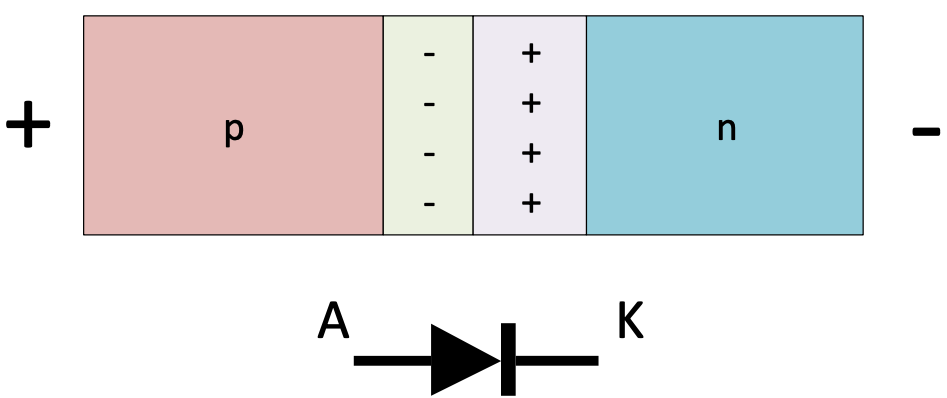
\includegraphics[scale=0.4,angle=0]{diodo.png}
\caption{Struttura e simbolo di un diodo in \textit{polarizzazione diretta}}
\end{figure}

Il diodo è formato da due terminali chiamati \textbf{anodo} e \textbf{catodo}, indicati con \textit{A} e \textit{K} e corrispondenti rispettivamente alla zona \textit{p} contente le lacune e alla zona \textit{n} contente gli elettroni. La freccia che compare nel simbolo del diodo indica il verso in cui scorre la \textit{corrente} (intesa come cariche positive): essa scorre dall'anodo verso il catodo. Se la corrente si muove dall'anodo verso il catodo significa che gli elettroni si spostano nel verso opposto: dal catodo all'anodo.

Come detto in precedenza, la barriera di potenziale che si viene a creare in corrispondenza delle due cariche nette e della giunzione impedisce agli elettroni di spostarsi dalla zona n alla zona p cioè dal catodo all'anodo. Tuttavia questo risulta essere vero fintanto che non si applica esternamente un certo \textit{potenziale}. In particolare, se si applica un potenziale \textit{positivo} all'anodo e \textit{negativo} al catodo ci si trova nelle condizioni di \textbf{polarizzazione diretta} tramite la quale il potenziale positivo applicato all'anodo fa alzare il potenziale della regione p e il potenziale negativo applicato al catodo fa abbassare il potenziale della regione n. Inoltre, fintanto che non c'è corrente all'interno della zona p non c'è caduta di potenziale, quindi il potenziale all'estrema sinistra è lo stesso potenziale del punto in cui inizia l'area con la carica negativa netta, lo stesso vale per la zona n. Con l'applicazione di potenziale esterno ai due estremi la curva tende a diventare sempre più piatta tendendo a diventare parallela all'asse \textit{x}; in queste condizioni gli elettroni e le lacune non incontrano più nessuna barriera di potenziale, quindi nessun ostacolo, e per questo sono liberi di fluire. Via via che si incrementa il potenziale in p e lo si abbassa in n, un po' di elettroni dal generatore esterno passano attraverso la zona n e vanno a neutralizzare la carica positiva netta. A questo punto, per effetto del \textit{bilanciamento} delle cariche, per ogni carica positiva che viene bilanciata a destra, un elettrone nella carica negativa netta si stacca e va verso il generatore passando attraverso la zona p e infine uscendo dal diodo Più questo processo va avanti e poi la regione di svuotamento diventa più stretta fino a svanire del tutto, una volta eliminata gli elettroni sono liberi di fluire.

Una volta raggiunta una certa tensione viene quindi annullata la barriera di potenziale e gli elettroni sono liberi di scorrere nel materiale pn. Dunque, applicando una tensione maggiore di una certa soglia inizia a scorrere corrente. Questa tensione soglia prende il nome di \textbf{tensione del diodo} (del potenziale interno che si era creato intorno alla giunzione pn con le due cariche nette opposte), viene indicata con $V_{D}$. Per un diodo al \textit{silicio} $V_D \approx 0,7\,V$, il che significa che se col generatore si supera la tensione di $0,7\,V$ si riesce ad annullare la barriera di potenziale nel mezzo del diodo pn e inizia a scorrere corrente con un andamento \textbf{esponenziale} con la tensione applicata al diodo:
\begin{equation}
    I_{D} = I_{0}\,(e^{(V_{D}/nV_{T})} - 1)
    \label{corrente_id}
\end{equation}
Per cui, fino a $0,7\,V$ non succede niente, superata tale soglia la corrente inizia a crescere esponenzialmente perché non incontra più nessun ostacolo.

Inizialmente si era detto che se non scorre corrente la parte di materiale p ed n non producono una caduta di tensione, però in realtà intrinsecamente le due parti di materiale p ed n sono anche \textit{conduttori} quindi presentano una loro certa \textbf{resistività}. Dunque se si volesse fare una rappresentazione veritiera del circuito, oltre al generatore e al diodo \textit{ideale} bisognerebbe aggiungere due \textbf{resistenze}: una lato anodo rappresentante la conducibilità del materiale p e una lato catodo rappresentante quella del materiale n. Da questa rappresentazione si può quindi vedere come nella realtà ai capi della giunzione arrivi meno tensione di quella effettiva. 

Sapendo che la tensione delle resistenze è data da $V = R \cdot I$, la curva è esponenziale un volta superata la soglia di $0,7\,V$ ma ad un certo punto la tensione che si genera per \textit{caduta resistiva} è così grande che la tensione ai capi del diodo non cresce più, a quel punto la corrente $I_{D}$ non sarà più esponenziale ma \textit{lineare}. Meno corrente il diodo è in grado di portare e tanto prima di entrerà nella regione a crescita lineare.

Nella norma la regione di tipo p e quella di tipo n non sono drogate in maniera omologa ma una delle due è molto più drogata dell'altra. Il più delle volte è la regione n ad essere più drogata della regione p, cioè vale che $N_{d} >> N_{a}$. In queste condizioni ci sono tanti portatori di tipo n nella zona n (inteso come densità) ma ci sono poche lacune nella zona p, quindi quando un elettrone passa nella zona p si trova in una sorta di mare deserto di lacune. Per questa situazione si parla di \textbf{portatori minoritari} intendo il fatto che i portatori, cioè le lacune, sono molto sparsi e questo comporta che si hanno fenomeni di diffusione degli elettroni nel lato p e sono fenomeni non simmetrici, cioè non si osservazione la stessa situazione anche per la lacune nel lato n. L'aspetto principale è che via via che nel diodo sono presenti elettroni, questi si vanno ad accumulare nella parte di tipo p causando un fenomeno detto di \textbf{accumulo di carica} che, si vedrà più avanti, ha un effetto indesiderato.
\\\\Le considerazioni fatte finora sono relative al caso di polarizzazione diretta in cui si applica un potenziale positivo all'anodo e uno negativo al catodo. Nel caso contrario, detto \textbf{polarizzazione inversa} in cui si applica un potenziale negativo all'anodo e uno positivo al catodo, riprendendo l'andamento del potenziale in figura \ref{grafici}, il potenziale negativo applicato all'anodo fa abbassare ulteriormente il potenziale della regione p e il potenziale positivo applicato al catodo fa alzare ancora di più il potenziale della regione n.
\begin{figure}[h]
\centering
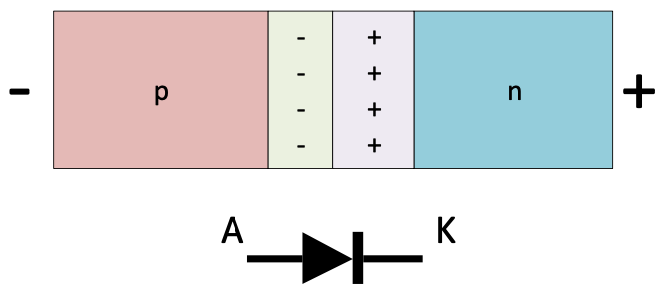
\includegraphics[scale=0.5,angle=0]{diodo_polarizzazione_inversa.png}
\caption{Diodo in \textit{polarizzazione inversa}}
\end{figure}
\\Questo comporta un aumento del valore assoluto della barriera di potenziale che diventerà più ripida. Inoltre, gli elettroni immessi nella zona p tramite il generatore esterno, si vanno ad aggiungere alla regione di svuotamento originale e, viceversa, nella zona n degli elettroni abbandonano la zona uscendo dal diodo. Il risultato netto è che la regione di svuotamento si \textit{allarga} con un corrispondente incremento della barriera di potenziale: i due rettangoli nel primo grafico di figura \ref{grafici} diventano più grandi, quindi aumenta anche il campo elettrico $E(x)$. Più aumenta la barriera di potenziale, più si accumulano cariche e più diventa difficile lo scorrimento della corrente attraverso il diodo. In realtà si ha comunque una corrente che scorre dal catodo all'anodo ed è definita dalla formula \eqref{corrente_id} che quindi vale sia per la polarizzazioni diretta che per quella inversa. In particolare, la corrente che scorre in polarizzazione inversa (anche detto \textbf{reverse bias}) è $I_{0}$ che è molto bassa (dell'ordine di $10^{-7} A$) ma comunque non nulla. Questa \textit{corrente di perdita} sarà tanto più piccola tanto più si sarà fatta attenzione nel progettare il diodo in modo tale che non ci sia e, generalmente, è proporzionale a quanta corrente può scorrere nel diodo nel caso di polarizzazione diretta o \textbf{forward bias}: diodi più grandi avranno corrente di perdita più grande e viceversa.

Il campo elettrico, come si vede nel secondo grafico di figura \ref{grafici}, ha il valore massimo in corrispondenza del confine tra la giunzione p e la giunzione n. In questo momento la parte centrale del diodo si comporta come un materiale \textbf{dielettrico} perché non conduce corrente a causa del fatto che le cariche sono tutte bloccate nella regione di svuotamento. Ma un materiale dielettrico non conduce corrente fino a quando non si supera la sua \textbf{rigidità dielettrica}. Il silicio ha un limite di rigidità dielettrica oltre la quale il materiale si \textit{rompe} (si dice che va in \textbf{breakdown}): il campo elettrico è così forte che le cariche elettriche da una parte vengono tirate dalla parte opposta fino ad essere \textit{strappate} dal reticolo cristallino e, a quel punto, inizia a scorrere corrente. Quindi il diodo, che in polarizzazione inversa non fa quasi scorrere corrente, una volta superata una certa soglia di rigidità dielettrica, detta \textbf{tensione di breakdown}, va in breakdown e da quel momento inizia a scorrere una corrente che cresce in maniera illimitata e improvvisa.
\begin{figure}[h]
\centering
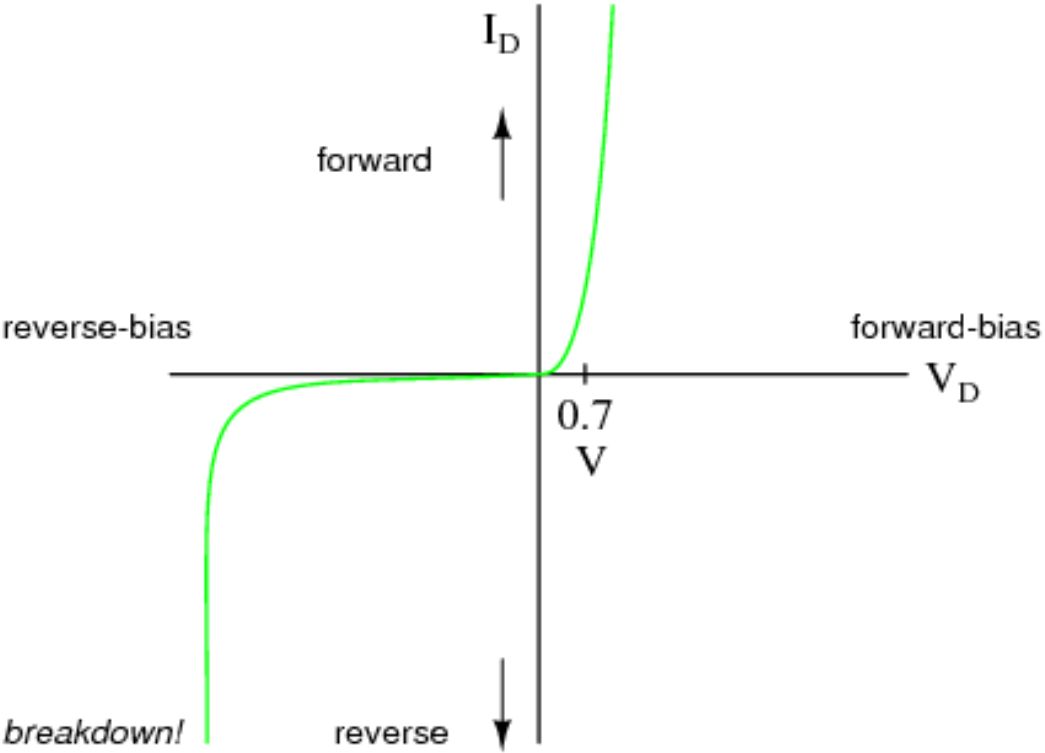
\includegraphics[scale=0.45,angle=0]{corrente_id.png}
\caption{Andamento della corrente nel diodo in polarizzazione diretta e inversa}
\label{i_diodo}
\end{figure}

In base a come sono costruiti diodo e circuito, il breakdown può essere \textit{reversibile}. Se all'interno del circuito (considerando un generatore ideale) la corrente non viene limitata in qualche modo (per esempio tramite delle resistenze) il diodo non è recuperabile dopo il breakdown. Ci sono due categorie di diodi: i diodi costruiti per andare in breakdown e quelli costruiti per non andarci; questi ultimi è molto probabile che effettivamente si rompano se vanno in breakdown indipendentemente dalla corrente. I diodi che invece sono costruiti appositamente per andare in breakdown sono chiamati \textbf{diodi Zener} e non si danneggiano andando in breakdown ma bisogna comunque limitare la corrente per esempio con una resistenza in serie per avere un corrente quasi lineare e quindi facilmente controllabile.
\begin{figure}[h]
\centering
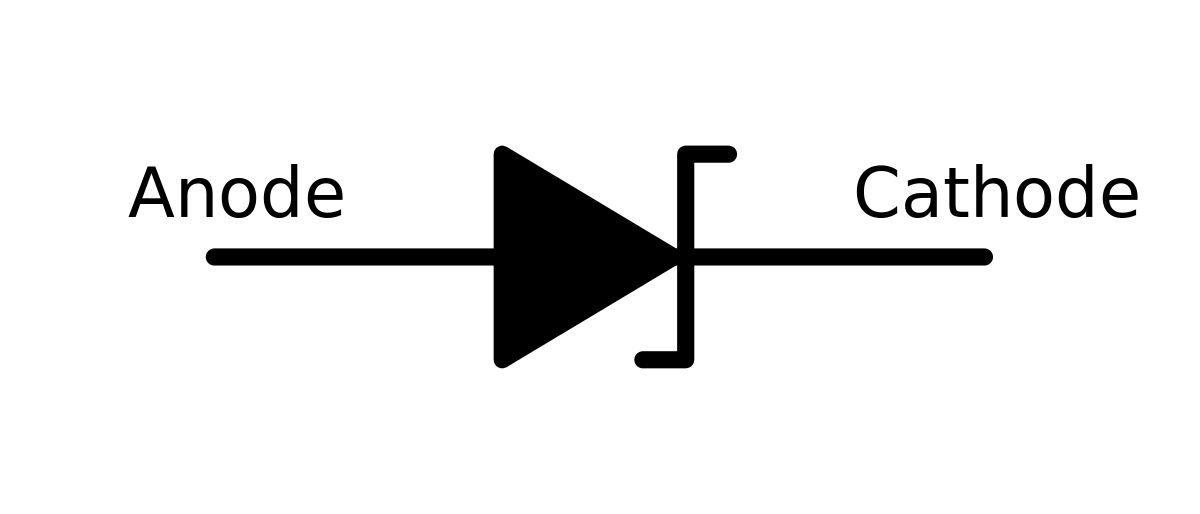
\includegraphics[scale=0.15,angle=0]{diodo_zener.png}
\caption{Simbolo del diodo Zener}
\end{figure}
\\In passato venivano usati per controllare la tensione ed è l'unico diodo che sopporta il breakdown inverso ma bisogna inserire una \textit{resistenza di limitazione}.\\

Nel contesto dell'elettronica digitale, in logica binaria, per una tensione $V_{D}$ compresa tra $0\,V$ e $0,7\,V$ si considera una corrente di $0\,A$ mentre oltre gli $0,7\,V$ si considera una corrente di $1\,A$, cioè infinita. Per tensioni negative, per $V_{D}$ compresa tra $0\,V$ e la tensione di breakdown si considera una corrente di $0\,A$ e oltre la tensione di breakdown si considera corrente infinitamente negativa. Nella realtà però il diodo è un dispositivo analogico caratterizzato da non avere cambi repentini di intensità di corrente.

\section{Diodi speciali}
Oltre al diodo Zener e ai diodi pn al silicio che si usano per controllare il verso di scorrimento della corrente, ci sono altre tipologie di diodi costruibili sfruttando ancora le proprietà dei materiali semiconduttori.
\begin{description}
    \item[Fotodiodo] È un dispositivo optoelettronico, cioè un dispositivo che sfrutta il dualismo tra energia e lunghezza d'onda (cioè tra fotone e l'energia che esso porta) per far sì che nel dispositivo a semiconduttore la luce che incide sul dispositivo stesso possa produrre degli effetti. A differenza di altri dispositivi optoelettronici che sono neri per non modificare il loro funzionamento a causa della luce, il fotodiodo è \textit{trasparente}. Il principio di funzionamento è del tutto analogo a quello della cella fotovoltaica: viene emessa corrente quando della luce incide sul fotodiodo. Per usarlo lo si polarizza in inversa e se della luce lo colpisce, se il fotone colpisce la regione di svuotamento, l'energia associata al fotone $e = \hbar \cdot \nu$ (con $\nu$ l'inverso della lunghezza d'onda) è in grado di prendere un elettrone nel reticolo cristallino e portarlo dalla \textbf{banda di valenza} nella \textbf{banda di conduzione} così che l'elettrone si stacca dalla sua lacuna, si crea una coppia elettone-lacuna liberi che è in grado di seguire il campo elettrico che si è creato tramite il quale la corrente scorre verso l'anodo, e si ha un passaggio di corrente. Quindi il diodo, che di base in polarizzazione inversa non conduce corrente, quando viene illuminato da una luce che abbia sufficiente energia per poter far passare gli elettroni dalla banda di valenza a quella di conduzione riesce a condurre corrente anche in condizioni di polarizzazione inversa. Si può usare per rilevare una radiazione luminosa incidente (per esempio in un telecomando a raggi infrarossi) oppure nei pannelli fotovoltaici in cui il pannello non è altro che un grande diodo pn al silicio e quando su di esso incide della luce solare diventa lui stesso un generatore di corrente con la corrente positiva uscente dall'anodo e la tensione che si genera ai capi del diodo che è sicuramente \textit{minore o uguale} della tensione di soglia del diodo stesso. Se la tensione che si genera fosse maggiore di $0,7\,V$ il diodo si polarizzerebbe direttamente e al suo interno vorrebbe scorrere una corrente contraria, dall'anodo al catodo. Normalmente una diodo al silicio per applicazioni fotovoltaiche genera tra gli $0,5$ e gli $0,6$ volt.
    \item[LED - Light Emitting Diode] Anche questo è un dispositivo optoelettronico che sostanzialmente ha un funzionamento opposto a quello del fotodiodo. È un dispositivo costruito in modo tale che quando viene polarizzato direttamente sia facile che nella regione di svuotamento si vadano a ricombinare elettroni e lacune; cioè è costruito in modo tale che gli elettroni che sono in banda di conduzione possano cadere in banda di valenza, così da poter liberare un fotone. La lunghezza d'onda del fotone liberato è \textit{inversamente proporzionale} all'energia (quindi la frequenza della radiazione luminosa emessa è direttamente proporzionale all'energia), quindi ad un salto energetico molto alto (barriera di potenziale alta) corrisponderà una lunghezza d'onda molto bassa cioè l'emissione del diodo si sposta verso gli ultravioletti; al contrario, se la barriera di potenziale è bassa l'emissione si sposta verso gli infrarossi. Accanto agli infrarossi c'è il \textit{rosso}, accanto agli ultravioletti c'è il \textit{viola}, nel mezzo partendo dal viola ci sono il blu, il verde, il giallo, l'arancione e infine il rosso. Dunque la lunghezza d'onda della luce emessa dal LED è esattamente determinata dalla sua distanza tra la banda di valenza e quella di conduzione, e a sua volta quella distanza è proporzionata dalla tensione che cade sul diodo, per questo il diodo LED è un diodo che normalmente ha una tensione di soglia \textit{molto alta}, soprattutto nel visibile e nell'ultravioletto. Inoltre, la tensione che cade ai capi del diodo, proprio perché è fatto per avere una barriera di potenziale grande, è tendenzialmente $> 1,5\,V$: per i LED \textit{rossi} è tipicamente $1,5\,V$, per i \textit{verdi} circa $1,8\,V$, per quelli \textit{blu} circa $2,2\,V$, per i diodi \textit{ultravioletti} è intorno ai $3\,V$, per i diodi \textit{infrarossi}, in particolare quelli nel vicino infrarosso, è circa $1,2\,V$. In ogni caso, la caduta di potenziale è proporzionata all'energia dell'emissione luminosa e tanto più l'emissione luminosa si sposta verso gli ultravioletti, tanto più è energetica e quindi tanto maggiore è la caduta di potenziale ai capi del diodo.
    \item[Diodo Shottky] Diodo particolare in cui la giunzione pn è fatta da un \textit{metallo} (per esempio l'\textit{alluminio} che è un materiale di $III^{a}$ colonna) nella zona p e da un \textit{semiconduttore} nella zona n. Questo accoppiamento fa sì che la regione di svuotamento si estenda solo nel lato del semiconduttore, nel metallo non esiste la regione di svuotamento perché la strutta molecolare di un metallo è il \textbf{mare di elettroni} in cui gli elettroni sono sempre liberi di muoversi: non si crea la regione di svuotamento ma il campo elettrico si. Questa caratteristica permette di avere una tensione di soglia \textit{minore} di quella di un diodo al silicio perché di fatto la regione di svuotamento è la metà di quella che si avrebbe normalmente. Come detto, mentre scorre corrente in un diodo normale si accumulano cariche minoritarie nella parte p.
    \begin{figure}[ht]
        \centering
        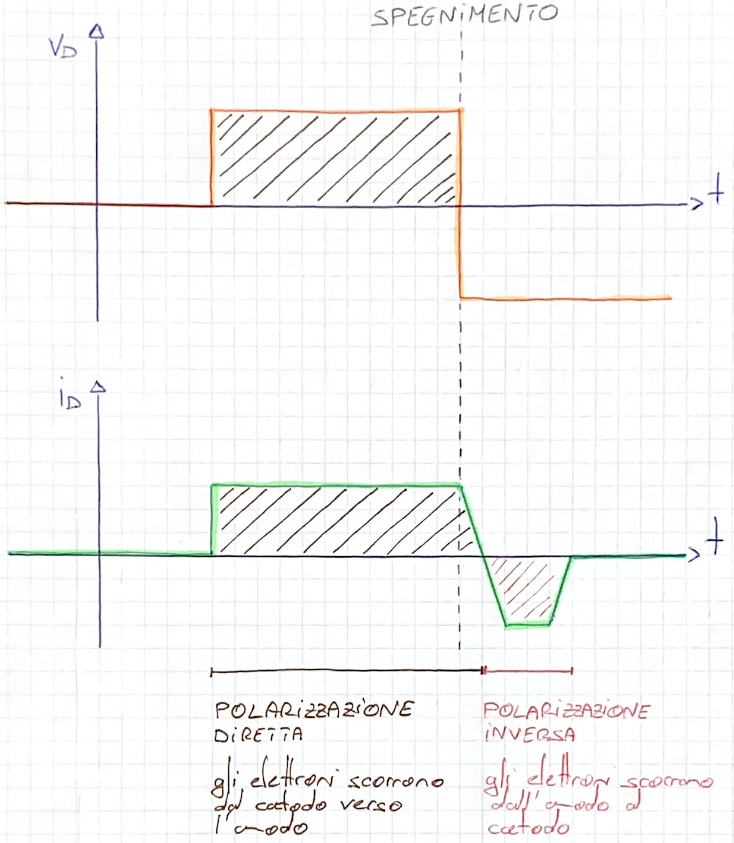
\includegraphics[scale=0.45,angle=0]{diodo_spegnimento.png}
        \caption{$V_{D}$ e $I_{D}$ di un diodo normale allo spegnimento}
    \end{figure}
    \\Questo comporta che quando si vuole spegnere il diodo, quindi $V_{D}$ diventa negativa perché si fa una polarizzazione inversa, esso si spegne lentamente, cioè $I_{D}$ scende lentamente ala valore previsto nel caso statico (invece si accende facilmente non appena viene polarizzato) perché ha accumulato cariche nella parte p che lo tengono ancora acceso. La corrente $I_{D}$ passa dall'essere positiva all'essere negativa per un certo tempo, fintanto che gli elettroni accumulati non vengono liberati. Indipendentemente dalla polarizzazione, passa comunque corrente. Tutto questo non succede nel diodo Shottky in cui, poiché la carica netta nella parte p non esiste, non esiste un accumulo di cariche bloccate nelle lacune e questo fa sì che quando il diodo passa in polarizzazione inversa si spegne immediatamente, cioè si comporta dinamicamente come un diodo ideale.
\end{description}

\chapter{BJT}
Il \textbf{BJT} viene così chiamato perché è un transistor bipolare, cioè composto da due poli. È un dispositivo a tre \textit{terminali} formato due due giunzioni: una giunzione np e una pn. I tre terminali sono: l'\textbf{emettitore} E, che costituisce la prima regione n a sinistra; la \textbf{base} B, corrispondente all'unica regione p presente e collocata nel mezzo; e infine il \textbf{collettore} C che invece è la seconda regione n collocata sulla destra del BJT.
\begin{figure}[h]
    \centering
    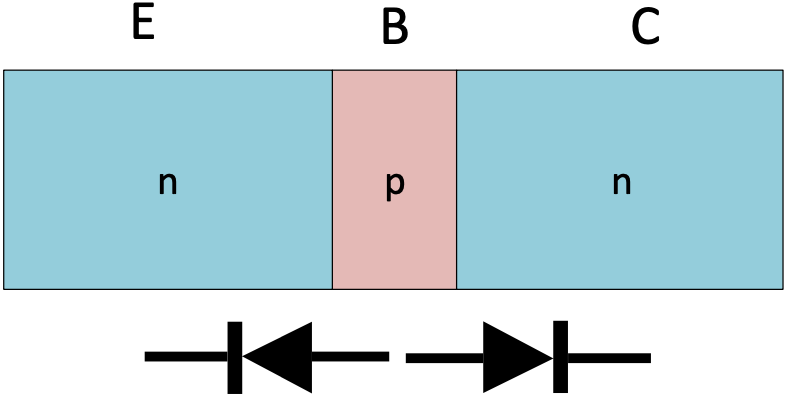
\includegraphics[scale=0.4,angle=0]{bjt_iniziale.png}
    \caption{Composizione di un BJT di tipo \textit{npn}}
    \label{bjt}
\end{figure}

Dalla rappresentazione schematica il BJT sembra un dispositivo simmetrico ma in realtà non lo è. Un aspetto importante è che la base è \textit{più stretta} dell'emettitore e del collettore, fondamentale per il suo funzionamento. Se fosse effettivamente costruito collegando due diodi in modo tale che le due zone p si tocchino, il dispositivo ottenuto non sarebbe un transistor perché due diodi così disposti, per l'equazione \eqref{giunzione_pn}, non producono nessun effetto perché non può scorrere corrente dall'emettitore al collettore in quanto è bloccata dal diodo np (emettitore - base) in quanto sarebbe polarizzato inversamente e analogamente non può scorrere corrente dal collettore all'emettitore perché bloccata dal diodo pn (base - collettore) polarizzato inversamente. Lo stesso vale nel caso di un BJT di tipo \textit{pnp}.
\begin{figure}[h]
    \centering
    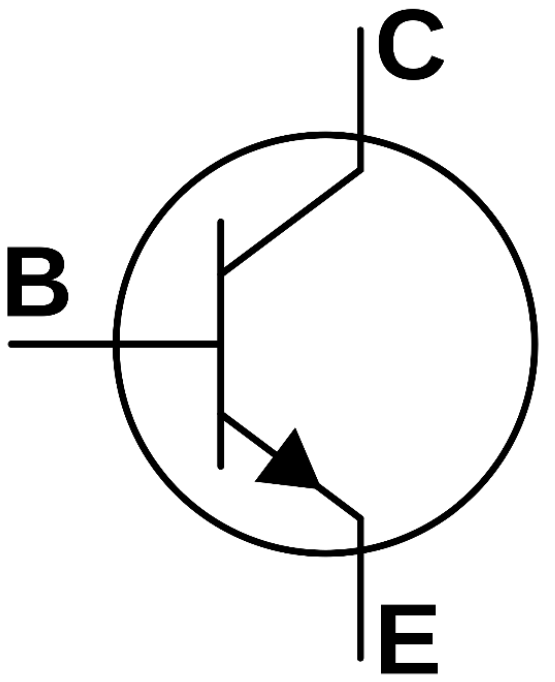
\includegraphics[scale=0.3,angle=0]{bjt_simbolo.png}
    \caption{Simbolo circuitale del BJT \textit{npn}}
\end{figure}

Nel simbolo circuitale del BJT la freccia indica la giunzione tra la base e l'emettitore. Nel caso del diodo classico a due terminali si prende \textit{positiva} la tensione dell'anodo e \textit{negativa} quella del catodo (quindi la tensione del diodo viene considerata positiva quando la tensione dell'anodo è positiva, ovvero il diodo è polarizzato direttamente); per il BJT si definiscono tre tensioni:
\begin{itemize}
    \item[$V_{be}$]: la tensione tra l'emettitore e la base che formano una giunzione pn. È \textit{positiva} quando la base è positiva rispetto all'emettitore perché $V_{be}$ è la differenza tra il potenziale (o tensione) della base $V_{b}$ (dove punta la freccia in figura \ref{tensioni_bjt}) e il potenziale dell'emettitore $V_{e}$ (dove parte la freccia). Quindi $V_{be} > 0$ significa che la giunzione tra emettitore e base è polarizzata \textit{direttamente}
    \item[$V_{bc}$]: la tensione tra la base e il collettore, è \textit{positiva} quando $V_{b} > V_{c}$ perché definita come differenza tra i potenziali $V_{b}$ e $V_{c}$
    \item[$V_{ce}$]: la tensione tra collettore ed emettitore, è \textit{positiva} quando $V_{c} > V_{e}$ perché definita come differenza tra i potenziali $V_{c}$ e $V_{e}$
\end{itemize}
\begin{figure}[h]
    \centering
    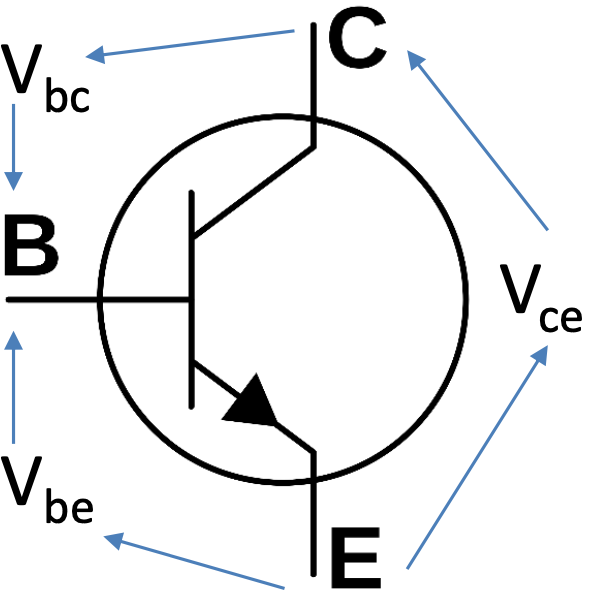
\includegraphics[scale=0.4,angle=0]{bjt_tensioni.png}
    \caption{Tensioni nel BJT \textit{npn}}
    \label{tensioni_bjt}
\end{figure}
Analogamente si hanno anche tre correnti, una per ognuno dei tre terminali del BJT:
\begin{itemize}
    \item[$I_{c}$]: la corrente del collettore, si prende \textit{positiva} quando è \textit{entrante} nel dispositivo
    \item[$I_{b}$]: la corrente di base, si prende \textit{positiva} quando è \textit{entrante} nel dispositivo
    \item[$I_{e}$]: la corrente dell'emettitore, si prende \textit{positiva} quando è \textit{uscente} nel dispositivo
\end{itemize}
Vale il principio di Kirchhoff per cui $I_{c} + I_{b} = I_{e}$.
\begin{figure}[h]
    \centering
    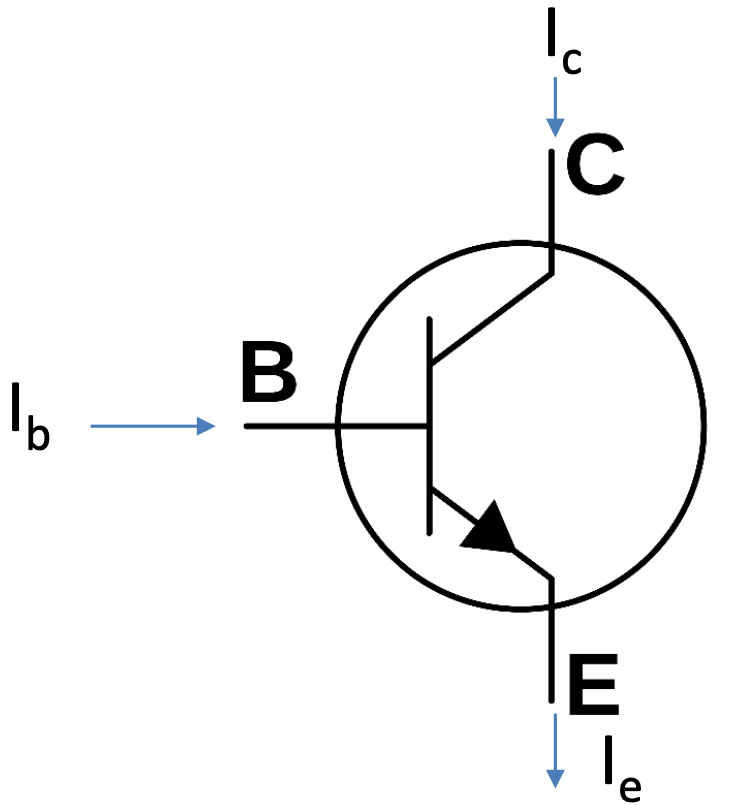
\includegraphics[scale=0.35,angle=0]{bjt_correnti.png}
    \caption{Correnti nel BJT \textit{npn}}
\end{figure}

\section{Regioni operative}
Il BJT è un dispositivo che può lavorare in \textit{quattro} modalità chiamate \textbf{regioni operative}: la regione di \textbf{cutoff} o \textbf{interdizione} in cui semplicemente il dispositivo è \textit{spento} e non sta facendo niente; la regione \textbf{attiva diretta}; la regione di \textbf{saturazione} e la regione \textbf{attiva inversa}. In tutte le regioni eccetto quella di cutoff il dispositivo fa qualcosa.

Si dice che il BJT è un \textbf{generatore di corrente controllato in corrente}, cioè le regioni di funzionamento sono determinate dalle correnti e/o dalle tensioni; in particolare ciò che guida il dispositivo è la corrente che entra in base $I_{b}$.

\subsection{Cutoff}
Nella regione di cutoff il transistor è spento, non passa corrente dal collettore all'emettitore. In questo caso \textit{entrambe} le giunzioni pn, BE tra la base e l'emettitore e BC tra la base e il collettore, sono polarizzate \textit{inversamente}, cioè sono in \textit{reverse bias}. Questo significa che:
\begin{equation*}
    V_{be} < V_{th} \text{ \, \, } V_{bc} < 0
\end{equation*}
con $V_{th}$ la tensione di soglia (anche detta potenziale di base). Per avere polarizzazione inversa tra base e collettore, il collettore deve avere un potenziale $V_{c}$ più alto rispetto al potenziale di base $V_{b}$. Questo succede finché il collettore non arriva ad avere un potenziale al massimo inferiore di $0,5\,V$ rispetto alla tensione di base, quindi o è una tensione molto elevata oppure è una tensione vicina alla tensione di base $V_{th}$ ma non sotto $0,5\,V$ rispetto a $V_{th}$ altrimenti si polarizzerebbe direttamente. Per le correnti, nella regione di cutoff si ha:
\begin{equation}
    I_{b} = 0\,A \text{ \, \, } I_{c} = 0\,A
\end{equation}
In realtà più che $0\,A$ sarà uguale ad una piccola corrente di perdita $I_{0}$ che è la corrente inversa della giunzione pn che si sta considerando.
\begin{figure}[h]
    \centering
    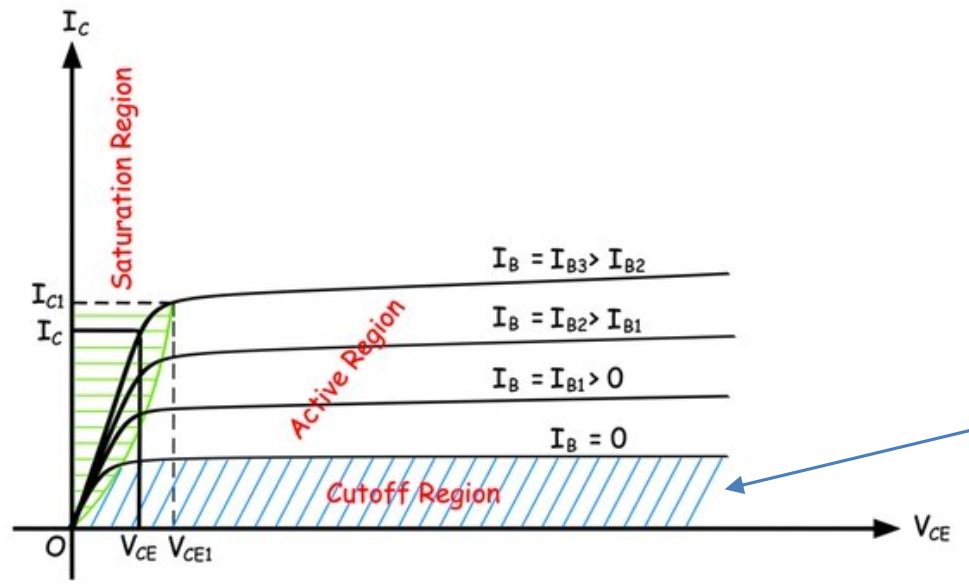
\includegraphics[scale=0.4,angle=0]{bjt_cutoff.png}
    \caption{Regione di cutoff}
\end{figure}

I grafici dei transistors hanno normalmente $V_{ce}$ nelle ascisse, $I_{c}$ nelle ordinate e le curve vengono disegnate al variare della \textit{variabile di controllo} che è $I_{b}$. Nella regione di cutoff si ha, come detto, $I_{b} = 0\,A$ e $I_{c} \approx I_{0}$ che è una corrente molto piccola.
\subsection{Attiva diretta}
Nella regione attiva diretta la giunzione BE tra la base e l'emettitore è polarizzata \textit{direttamente} quindi:
\begin{equation*}
    V_{be} > V_{th} \text{ \, \, } I_{b} > 0
\end{equation*}
La giunzione BC tra la base e il collettore è invece in polarizzazione \textit{inversa}:
\begin{equation*}
    V_{bc} < 0
\end{equation*}
cioè il potenziale del collettore è alto, maggiore di quello della base. Sotto queste condizioni ($I_{b} > 0 $ e $V_{bc} < 0$) il dispositivo si comporta come un transistor, cioè come un generatore di corrente controllato in corrente:
\begin{equation}
    I_{c} = h_{fe} \cdot I_{b}
    \label{corrente_attiva_diretta}
\end{equation}
dove $h_{fe}$ è una costante il cui valore è normalmente molto maggiore di zero (dell'ordine delle decine o centinaia) ed è chiamata \textbf{guadagno in corrente} del transistor. Dunque, la polarizzazione diretta della giunzione BE fa sì che scorra corrente dalla base all'emettitore (ovvero elettroni dall'emettitore alla base) e la polarizzazione inversa della giunzione BC alza il potenziale del collettore facendo sì che scorra una corrente molto maggiore dal collettore all'emettitore.
\begin{figure}[h]
    \centering
    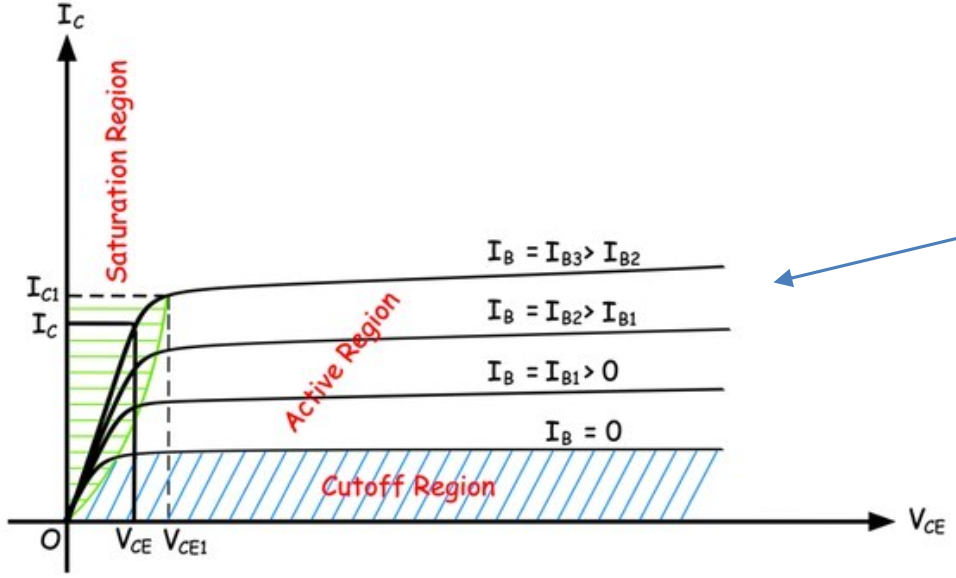
\includegraphics[scale=0.4,angle=0]{bjt_attiva_diretta.png}
    \caption{Regione attiva diretta}
    \label{attiva_diretta}
\end{figure}

Si è detto inizialmente che la base del BJT è più stretta rispetto agli altri due terminali. Polarizzando direttamente BE si crea un potenziale positivo nella base $V_{b} > 0$ e negativo nell'emettitore $V_{e} < 0$, quindi scorre corrente dalla base verso l'emettitore ed elettroni dall'emettitore alla base. Inoltre, la tensione del collettore è molto maggiore di quella di base $V_{c} >> V_{b}$ quindi la giunzione pn BC è polarizzata inversamente. Normalmente la giunzione BC sarebbe un diodo, quindi non ci sarebbero elettroni disponibili nella regione p della base per andare nella regione n del collettore perché tra le due c'è una regione di svuotamento e c'è una differenza di potenziale. Il fatto che la base sia molto stretta, che il potenziale del collettore sia molto elevato e che l'emettitore stia emettendo elettroni verso la base fa sì che nel momento in cui un elettrone passa dall'emettitore alla base tale elettrone diventa disponibile (nella zona p c'è scarsità di elettroni) e, grazie al potenziale molto elevato dal collettore, viene attirato e trasportato nella regione del collettore e da lì risale nella corrente arrivando fino al collettore stesso. Quindi gli elettroni della giunzione BE, che erano destinati a rientrare verso la base come avviene in una qualsiasi giunzione pn, in realtà prima di ricombinarsi vengono catturati dal campo elettrico del collettore che li strappa dalla ricombinazione così da saltare la base e andare direttamente nella regione n del collettore. In un transistor la base viene quindi fatta sottile per evitare la ricombinazione degli elettroni nella base in modo che vadano invece nel collettore.

Tutto questo processo è \textit{ragionevolmente efficiente} il che vuol dire che una percentuale molto elevata degli elettroni (per esempio 99 elettroni su 100) provenienti dall'emettitore salta la base per andare nell'emettitore e solo una piccola percentuale si ferma nella base, ovvero:
\begin{equation*}
    \frac{I_{c}}{I_{b}} \approx 99
\end{equation*}
cioè 99 elettroni vanno nel collettore e 1 nella base. Il guadagno in corrente del transistor è:
\begin{equation*}
    \frac{I_{e}}{I_{b}} \approx 100
\end{equation*}
Se il guadagno del transistor fosse 50 significa che 2 elettroni rimangono in base e 98 vanno nel collettore. I guadagni medi dei transistor sono molto elevati.

Tutto questo processo però finisce nel momento in cui non c'è più un sufficiente potenziale nel collettore per attirare gli elettroni. A quel punto gli elettroni rimangono all'interno della base, si ricombinano e si passa alla saturazione. 

Per una tensione del collettore abbastanza elevata (quindi per $V_{ce}$ grande) la corrente del collettore $I_{c}$ è \textit{lineare} (regione attiva diretta - figura \ref{attiva_diretta}), ma nel momento in cui il potenziale del collettore diventa piccolo la corrente del collettore tende a zero (regione di saturazione - figura \ref{saturazione}). Sotto un certo livello di tensione del collettore, che si prende intorno ai $ 0,2 - 0,3\,V$, si considera il dispositivo come in saturazione.

\subsection{Saturazione}
Nella regione di saturazione sia la giunzione tra la base e l'emettitore che quella tra la base e il collettore sono \textit{entrambe} in  polarizzazione \textit{diretta}. A differenza del caso precedente in cui il potenziale del collettore era molto elevato e per questo $V_{bc} < 0$ e poteva scorrere molta corrente secondo l'equazione \eqref{corrente_attiva_diretta}, adesso si abbassa il potenziale del collettore a circa $ 0,2 - 0,3\,V$ quindi inferiore al potenziale della base. Quindi la giunzione BC è polarizzata direttamente perché la tensione del collettore è circa $0,2\,V$, quella della base è di $0,8\,V$ e dunque $V_{bc} = 0,6\,V$. Tutto questo comporta che la corrente del collettore diminuisce e diventa minore strettamente della massima possibile in regione attiva diretta, cioè:
\begin{equation}
    I_{c} < h_{fe} \cdot I_{b}
\end{equation}
Si dice che il transistor \textit{ha saturato} cioè la tensione del collettore $V_{c}$ è diventata così bassa che non è più in grado di far scorrere le cariche. Per il resto, si ha:
\begin{equation*}
    V_{be} > V_{th} \text{ \, \, } V_{ce} < V_{ce-sat} \text{ \, \, } I_{b} > 0
\end{equation*}
\begin{figure}[h]
    \centering
    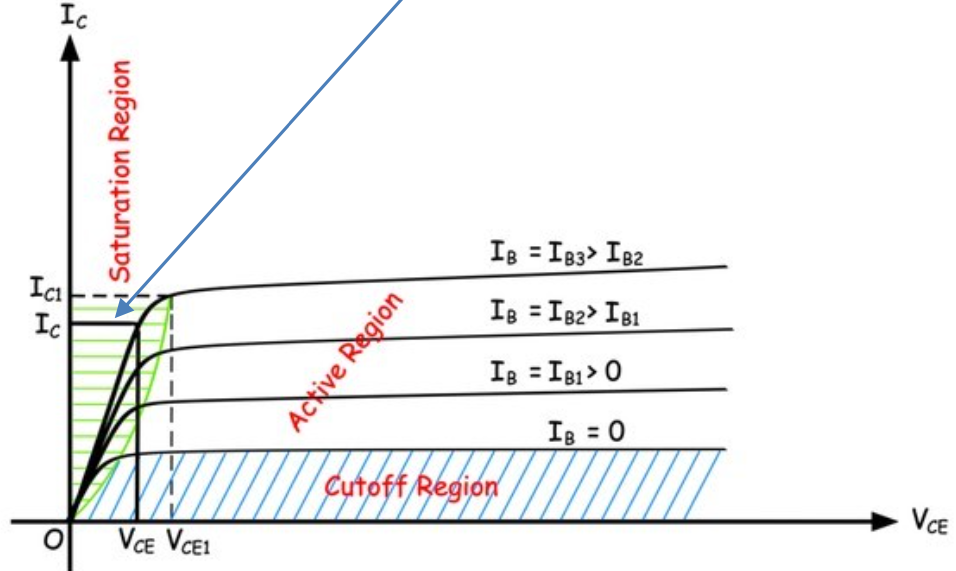
\includegraphics[scale=0.37,angle=0]{bjt_saturazione.png}
    \caption{Regione di saturazione}
    \label{saturazione}
\end{figure}

\subsection{Attiva inversa}
Nella regione attiva inversa la giunzione BC tra la base e il collettore è polarizzata \textit{direttamente}, mentre la giunzione BE tra la base e l'emettitore è polarizzata \textit{inversamente}. È sostanzialmente come nella regione attiva diretta ma con ruoli scambiati per il collettore e l'emettitore. Questo comporta che:
\begin{equation*}
    V_{be} < 0 \text{ \, \, } V_{ce} < V_{th}
\end{equation*}
Tuttavia in questa situazione si ha:
\begin{equation}
    I_{e} \approx -\,I_{b}
\end{equation}
cioè il guadagno in corrente del transistor è:
\begin{equation*}
    \frac{I_{e}}{I_{b}} \leq 1
\end{equation*}
questo perché il collettore \textit{non è bravo} come l'emettitore ad emettere elettroni e, viceversa, l'emettitore \textit{non è bravo} come il collettore a collezionare elettroni. 
\begin{figure}[h]
    \centering
    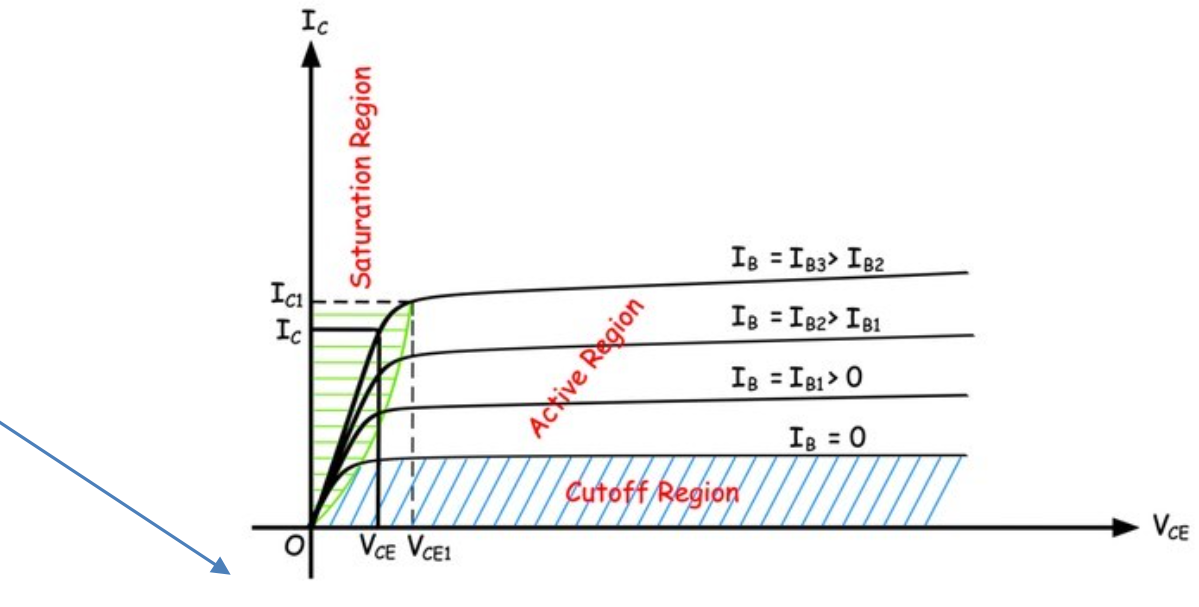
\includegraphics[scale=0.4,angle=0]{bjt_attiva_inversa.png}
    \caption{Regione attiva inversa}
\end{figure}

\section{Layout fisico}
Il BJT non è un dispositivo con una struttura simmetrica tra i tre terminali che lo compongono, ovvero non ha la struttura rappresentata in figura \ref{bjt}. In realtà, la sua realizzazione (effettuata su dei \textit{wafer}, sottili fette di materiale semiconduttore) prevede la creazione di sacche di drogante sia di tipo p che di tipo n.
\begin{figure}[h]
    \centering
    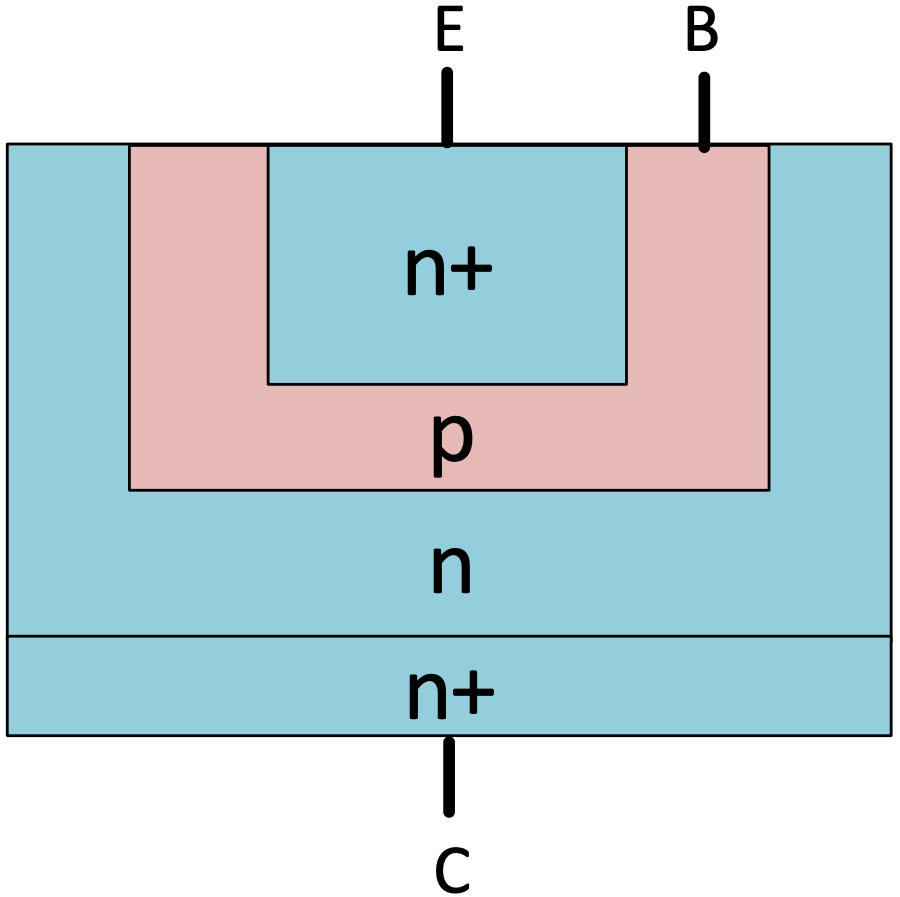
\includegraphics[scale=0.3,angle=0]{bjt_layout.png}
    \caption{Layout fisico di un BJT \textit{npn}}
\end{figure}
\\La regione n+ in basso serve semplicemente per la \textit{metallizzazione} del collettore. Il transistor vero e proprio è costituito da: l'emettitore (normalmente drogato \textbf{n+} dove il + sta a significare che è \textit{molto} drogato), la base (sottile, circonda l'emettitore, è drogata p) e il collettore (drogato n, circonda tutto l'emettitore). In questa configurazione l'emettitore, piccolo ma molto drogato, è facilmente generatore di elettroni e quando emette elettroni questi sono facilmente catturati dal collettore. Viceversa, se si polarizza in \text{attiva inversa} il dispositivo, il collettore può emettere elettroni ma, essendo un silicio drogato di tipo n e non n+, ne emette pochi e, per di più, ha una disposizione sfavorevole a causa della quale i pochi elettroni emessi hanno pochissima probabilità di essere catturati dall'emettitore mentre è molto più probabile che si ricombinino in base. È questo il motivo (asimmetria sia di drogaggio - n+ contro n - che di geometria) per cui il guadagno in regione attiva inversa è molto più piccolo del guadagno in regione attiva diretta.

\section{BJT pnp}
È il dispositivo perfettamente \textit{complementare} rispetto al BJT npn visto finora perché si ottiene scambiando i drogaggi: in questo transistor la base è drogata di tipo n mentre emettitore e collettore sono entrambi drogati di tipo p.
\begin{figure}[h]
    \centering
    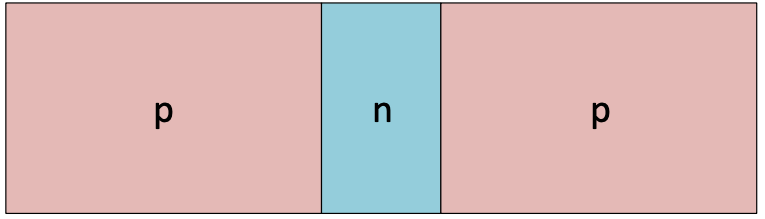
\includegraphics[scale=0.45,angle=0]{bjt_pnp.png}
    \caption{Struttura di un BJT di tipo \textit{pnp}}
\end{figure}

Nell'essere complementare al BJT npn si vanno a considerare le stesse equazioni del BJT pnp ma si usa una notazione di \textit{segno opposto} per le tre tensioni e correnti che caratterizzano il dispositivo.

Per le tensioni si considera \textit{positiva} la giunzione BE tra la base e l'emettitore quando il potenziale dell'emettitore è maggiore di quello della base ($V_{be} = V_{e} - V_{b}$ la freccia va dalla base all'emettitore), si considera \textit{positiva} la giunzione BC tra la base e il collettore quando il potenziale del collettore è maggiore di quella della base ($V_{bc} = V_{c} - V_{b}$ la freccia va dalla base al collettore), infine si considera \textit{positiva} la giunzione EC tra emettitore e collettore quando il potenziale dell'emettitore è maggiore di quello del collettore ($V_{ce} = V_{e} - V_{c}$ la freccia va dal collettore all'emettitore).

Per le correnti si considera \textit{positiva} la corrente entrante nell'emettitore e di conseguenza \textit{negative} le correnti uscenti dalla base e dal collettore.
\begin{figure}[h]
    \centering
    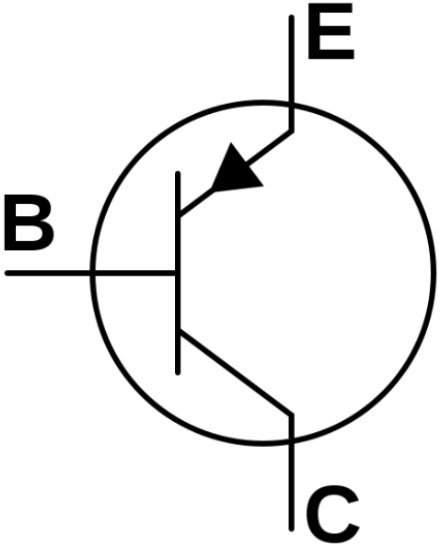
\includegraphics[scale=0.4,angle=0]{bjt_pnp_simbolo.png}
    \caption{Simbolo circuitale di un BJT \textit{pnp}}
\end{figure}

Le regioni operative sono le stesse del BJT npn: nella regione \textit{attiva diretta} la giunzione BE è polarizzata \textit{direttamente} cioè la tensione della base è più bassa di quella dell'emettitore e il collettore ha una tensione molto più bassa rispetto a base ed emettitore (infatti nel simbolo circuitale si dispongono i tre terminali per potenziale sempre più basso spostandosi dall'alto verso il basso - così la corrente andrà dall'alto verso il basso).

Nel BJT npn si parla di elettroni come portatori di carica, nel transistor pnp invece si parla di lacune che fungono da portatori di carica.

A livello statistico per definire il guadagno si deve tenere conto della \textbf{mobilità dei portatori}, ovvero quanto i portatori (che sono generati dall'emettitore) si muovono facilmente all'interno del materiale. Lacune ed elettroni non hanno la stessa mobilità, in particolare le lacune si muovono con una mobilità che è circa la \textit{metà} di quella con cui si muovono gli elettroni. Quindi dati due dispositivi geometricamente uguali ma con drogaggi tutti simmetricamente opposti, uno che sfrutta il moto degli elettroni come portatori di carica e l'altro che sfrutta il moto delle lacune, il dispositivo che sfrutta il moto delle lacune in genere sperimenta un guadagno in corrente che è circa la \textit{metà} di quello del dispositivo che sfrutta il modo degli elettroni. In questo caso, i transistor pnp hanno come portatori le lacune (essendo l'emettitore drogato p) che, muovendosi più lentamente, tendono più facilmente a ricombinarsi quando passano nella base e quindi il guadagno del dispositivo è minore rispetto a quello che si potrebbe ottenere con un transistor npn.\\

Riassumendo, per entrambi le tipologie di transistor bipolari si identificano quattro regioni operative:
\begin{description}
    \item[Cutoff] la giunzione base - emettitore è interdetta quindi non passa corrente né nella giunzione BE né in quella BC
    \item[Attiva diretta] la giunzione BE è polarizzata direttamente, quindi scorre corrente, mentre la giunzione BC è polarizzata inversamente. Il potenziale del collettore è molto elevato in valore assoluto e quindi il dispositivo si comporta come una sorgente di corrente controllata in corrente, dove il controllo è effettuato dalla corrente della base $I_{b}$, la sorgente di corrente è la corrente del collettore $I_{c}$ e il guadagno in corrente è $h_{fe}$
    \item[Saturazione] si ottiene abbassando progressivamente il valore assoluto del potenziale del collettore. Non c'è più possibilità di generare in modo costante tutta la corrente generata in regione attiva diretta, la corrente quindi diminuisce e la tensione può scendere fino ad un valore che generalmente è detta \textbf{tensione di saturazione} che vale $V_{ce-sat} \approx 0,2,\,V - 0,3\,V$. Il transistor non è più in grado di assorbire corrente
    \item[Attiva inversa] la giunzione BE è polarizzata inversamente e la giunzione BC è polarizzata direttamente. Si ottengono valori di guadagno di corrente molto bassi e minori o uguali di 1, passa poca corrente
\end{description}
\section{Fototransistor}
Un particolare dispositivo appartenente alla famiglia dei dispositivi optoelettronici insieme al fotodiodo è il \textbf{fototransistor}. Questo dispositivo è generalmente un transistor di tipo \textit{npn} con la particolarità che il terminale di base è \textit{assente}. Per polarizzare \textit{direttamente} la giunzione BE tra la base e l'emettitore si deve iniettare una \textbf{fotocorrente} invece di una corrente vera e propria. Per farlo vengono mandati dei fotoni sulla base del dispositivo e, una volta illuminata, per effetto dei fotoni vengono generate coppie elettrone-lacuna e queste coppie, se il collettore ha un potenziale sufficientemente elevato, generano una fotocorrente che scorre dalla base all'emettitore e che a sua volta si traduce in una molto maggiore corrente che scorre dal collettore all'emettitore. Questo significa che se $V_{c}$ è sufficientemente grande, il fototransistor è \textit{sempre} in regione \textit{attiva diretta}.
\begin{figure}[h]
    \centering
    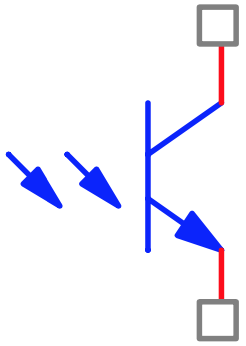
\includegraphics[scale=0.5,angle=0]{phototransistor.png}
    \caption{Simbolo circuitale di un fototransistor}
\end{figure}

Il vantaggio di questo dispositivo, che è sicuramente più complesso di un fotodiodo, è che si ha sempre un dispositivo a due terminali (come detto la base è assente) però la corrente che scorre in questo dispositivo è $h_{fe}$ volte la corrente che scorre nel relativo fotodiodo; il tutto a parità di luce incidente.

Viene utilizzato attaccando una resistenza al collettore (indicata con $R_{c}$) così da ottenere la tensione di polarizzazione del collettore $V_{cc}$, l'emettitore si mette a massa e la tensione di uscita $V_{out}$\, è quella del collettore. Sapendo che $I_{c} = h_{fe} \cdot I_{b}$ e che $I_{b}$ è proporzionale a $P_{in}$, la potenza luminosa in ingresso, si ottiene:
\begin{equation*}
    V_{out} = V_{cc} - ( R_{c} \cdot h_{fe} \cdot I_{b})
\end{equation*}
dove il termine $h_{fe} \cdot I_{b}$ viene visto come un unico termine, cioè $I_{c}$, che è ricavabile dal datasheet del fototransistor ed è generalmente centinaia di volte più grande dell'analogo per un fotodiodo. Oppure si può mettere la resistenza collegata non con il collettore ma con l'emettitore; in questo caso $V_{out}$ è la tensione dell'emettitore e vale $V_{out} =  R_{e} \cdot P_{in} \cdot G$ con \textit{G} il guadagno del fototransistor. Questi dispositivi si trovano all'interno dei telecomandi, dispositivi che in genere lavorano con gli infrarossi.

\chapter{MOS}
Il \textbf{MOS} è un dispositivo appartenente alla famiglia dei \textbf{FET}, ovvero dei \textit{transistors ad effetto di campo}, realizzato con tecnologia \textbf{metallo}, \textbf{ossido} e \textbf{semiconduttore}. Come per i BJT, anche per i MOS esistono due varianti: gli \textbf{N-MOS} e i \textbf{P-MOS}, rispettivamente a portatori elettroni e a portatori lacune. A differenza dei BJT che sono dispositivi controllati in corrente, i MOS sono dispositivi \textbf{controllati in tensione}. È per questo motivo che sono dei FET, perché è il campo elettrico che determina il funzionamento di questi dispositivi.

È un dispositivo a tre terminali, disposti come i tre terminali del transistor, e chiamati: \textbf{drain} (corrispondente al collettore del transistor), \textbf{gate} (corrispondente alla base) e \textbf{source} (corrispondente all'emettitore).

Le tensioni tra i tre terminali e le correnti sono definite nello stesso modo dei BJT. In particolare, i versi e i segni in un N-MOS sono definiti come nei BJT di tipo npn mentre in un P-MOS come in quelli di tipo pnp.

\section{N-MOS}
Un \textbf{N-MOS} è anche chiamato \textbf{mosfet a canale n}. È un dispositivo controllato in tensione nel senso che è la tensione di gate $V_{gs}$ a controllarne il funzionamento.
\begin{figure}[h]
    \centering
    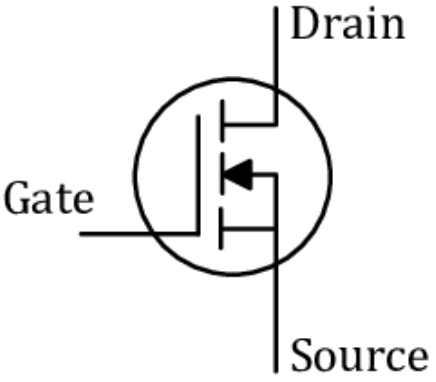
\includegraphics[scale=0.5,angle=0]{n_mos_simbolo.png}
    \caption{Simbolo circuitale di un N-MOS}
\end{figure}
\\Le tensioni sono definite come segue:
\begin{itemize}
    \item[$V_{sd}$]: la tensione tra drain e source. È \textit{positiva} quando drain è positivo rispetto a source, cioè quando $V_{d} > V_{s}$ perché $V_{ds}$ è la differenza tra il potenziale del drain $V_d$ e quello del source $V_s$
    \item[$V_{gs}$]: la tensione tra gate e source. È \textit{positiva} quando gate è positivo rispetto a source, cioè quando $V_{g} > V_{s}$
    \item[$V_{dg}$]: la tensione tra drain e gate. È \textit{positiva} quando gate è positivo rispetto a drain, cioè quando $V_{g} > V_{d}$
\end{itemize}
Analogamente le tre correnti, una per ognuno dei tre terminali del MOS, sono:
\begin{itemize}
    \item[$I_{d}$]: la corrente del drain, si prende \textit{positiva} quando è \textit{entrante} nel dispositivo
    \item[$I_{g}$]: la corrente del gate, si prende \textit{positiva} quando è \textit{entrante} nel dispositivo
    \item[$I_{s}$]: la corrente del source, si prende \textit{positiva} quando è \textit{uscente} dal dispositivo
\end{itemize}
La particolarità di un N-MOS è che la corrente del gate $I_{g}$ è \textit{sempre nulla} in tensione \textit{continua}. Questo aspetto è fondamentale per i dispositivi a basso consumo perché un dispositivo che consuma poco è un dispositivo nel quale, possibilmente, non ci sono correnti che scorrono continuamente. Tenere acceso un circuito logico composto da tanti transistors BJT necessita di polarizzare le loro basi con delle correnti (seppur minime), quindi consuma corrente. Al contrario, un circuito logico realizzato con dispositivi MOS ha la capacità di non consumare corrente quando non ci sono transizioni o di consumarne poca quando ce ne sono poche.
\begin{figure}[h]
    \centering
    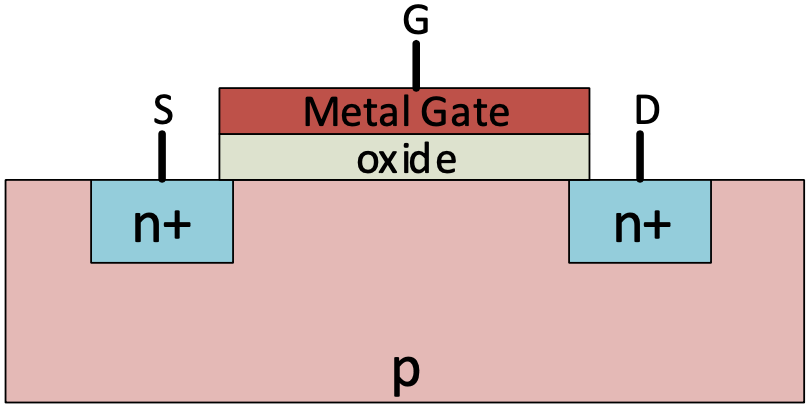
\includegraphics[scale=0.4,angle=0]{n_mos_struttura.png}
    \caption{Struttura di un N-MOS}
    \label{struttura_nmos}
\end{figure}
\\Un MOSFET a canale n è composto da una zona in silicio con drogaggio di tipo p sulla quale sono presenti due zone drogate n+ utilizzate per favorire la \textbf{metallizzazione} con l'esterno e in corrispondenza di queste due zone drogate n+ sono presenti i terminali source e drain.

La metallizzazione è necessaria perché gli scambi tra il dispositivo e l'esterno avvengono tramite i contatti esterni in alluminio e per far sì che avvenga la comunicazione tra dispositivo ed esterno si deve permettere di avere una giunzione che non sia \textit{raddrizzante}, ovvero che non sia una giunzione di tipo pn. Un materiale n+ (sopratutto se è molto n+), messo in contatto con l'alluminio che è un metallo, permette di creare una giunzione detta \textbf{ohmica} che non è raddrizzante.

È poi presente uno strato di \textbf{ossido} di dimensioni molto limitate (frazioni del micron) che viene utilizzato nell'industria dei semiconduttori come materiale \textit{isolante} e viene generalmente realizzato in \textit{biossido di silicio} oppure in \textit{nitruro di silicio}, entrambi forme vetrose del silicio altamente isolanti. Quindi questo strato di ossido ha un aspetto vetroso e una rigidità dielettrica, cioè un potere isolante, come quella del vetro (molto isolante). Su questo strato di ossido è poggiato un metallo che costituite il terzo terminale: il gate.

La sequenza di materiali: semiconduttore di tipo p, ossido e metallo definisce proprio la struttura MOS caratteristica di questi dispositivi.

Dal gate in metallo al semiconduttore di tipo p \textit{non} può scorrere corrente perché tra di loro è presente lo strato di ossido isolante. È questo il motivo per cui, in condizione di tensione continua, la corrente del gate è sempre nulla: perché non scorre corrente continua dal gate alla zona p. 

Tuttavia, questa struttura è a sua volta una struttura di materiali conduttori separati da un isolante a facce piane e parallele (nello specifico un conduttore e un semiconduttore paralleli e separati da uno strato isolante), cioè è un \textbf{condensatore} e questo comporta che, variando la tensione ai capi del condensatore o passando in tensione \textit{alternata}, ci saranno delle cariche che scorreranno, ovvero sui transitori ci sarà effettivamente della corrente che servirà per caricare e scaricare la \textit{capacità equivalente} del gate.

\section{Funzionamento}
Per costruzione, in condizioni stazionarie tra source e drain non può passare corrente perché i due terminali sono collegati tramite due giunzioni pn simmetriche disposte come in un BJT di tipo npn, cioè due diodi opposti uno dei quali è sempre polarizzato inversamente. Rispetto alla struttura transistor, la zona p, chiamata \textbf{canale}, non è stretta e questo comporta che la separazione tra le due zone n è molto pronunciata.

Un N-MOS inizia a funzionare nel momento in cui si va ad applicare una tensione di gate \textit{positiva} cioè $V_{gs} > 0$ rispetto al resto del circuito (in particolare rispetto al materiale di tipo p). Ciò che succede quando si applica una tensione positiva al gate è esattamente che succede all'interno di un condensatore: sulla piastra soggetta al potenziale positivo, corrispondente al gate, si accumulano le cariche positive, mentre sulla piastra opposta, la porzione del semiconduttore di tipo p a contatto con lo strato di ossido, vengono attratte cariche negative. Queste cariche negative accumulate vanno ad occupare gli spazi disponibili delle lacune che quindi vengono riempite con portatori di elettroni (come succedeva nella giunzione pn) e si crea una \textbf{regione di svuotamento}.
\begin{figure}[h]
    \centering
    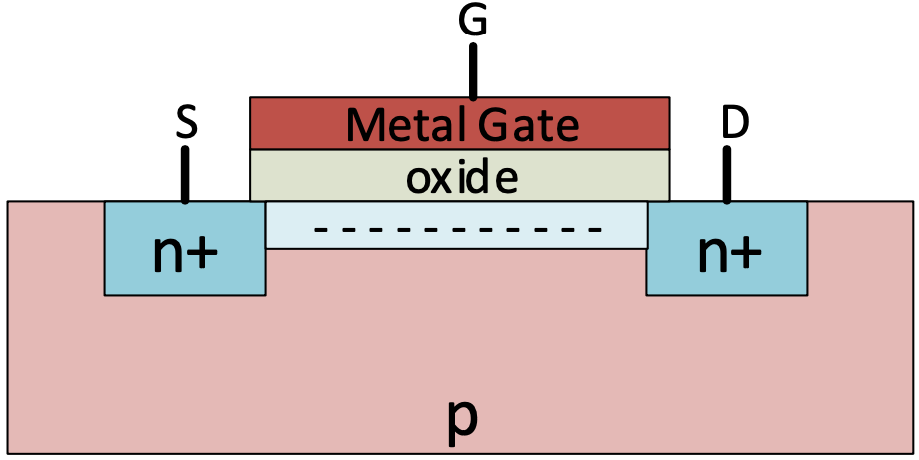
\includegraphics[scale=0.4,angle=0]{n_mos_svuotamento.png}
    \caption{Accumulo della cariche negative}
\end{figure}
\\Essendosi creata un regione di svuotamento, le cariche sono tutte bloccate dentro le lacune libere e questo comporta che non si possano avere fenomeni di scorrimento di cariche: ci si trova ancora in una situazione di stazionarietà.

Continuando ad aumentare la tensione di gate $V_{gs}$, questa finirà per superare un certo valore di soglia $V_t$. Quando $V_{gs} > V_t$ il campo elettrico che si forma all'interno del condensatore è così elevato che riesce a tirare ulteriori elettroni prendendoli dalle due zone a drogaggio n+ e portandoli nella zona p nella quale si erano già accumulate delle cariche negative.
\begin{figure}[h]
    \centering
    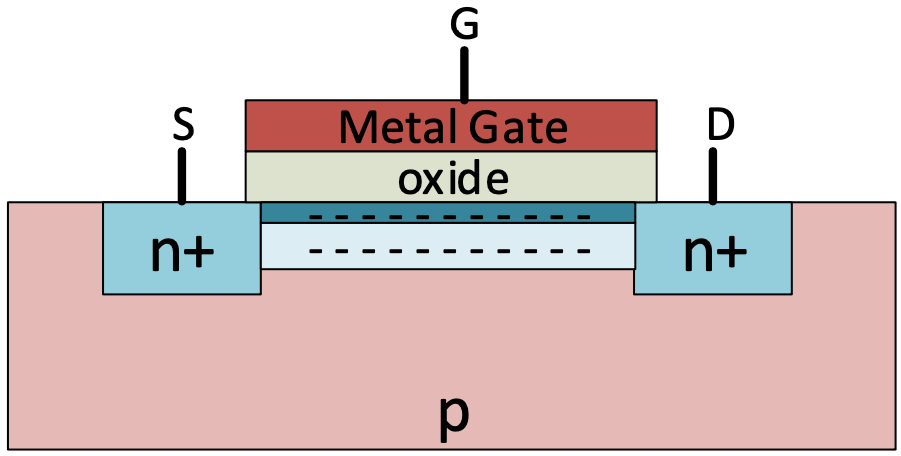
\includegraphics[scale=0.4,angle=0]{n_mos_canale.png}
    \caption{Accumulo della cariche negative}
    \label{svuotamento}
\end{figure}
\\Questi ulteriori elettroni (provenienti sopratutto dal source perché si sta applicando una differenza di potenziale $V_{gs} = V_{g} - V_s$ tra gate e source per utilizzare il source come connessione al terzo terminale: il drain) sono tutti elettroni \textit{liberi}, cioè sono elettroni in eccesso rispetto a quelli che avevo riempito il reticolo cristallino inserendosi nelle lacune per creare la regione di svuotamento e si vanno a disporre al di sotto del gate. A questo punto si è creato un \textbf{canale conduttivo } di elettroni tra source e drain, cioè una zona che sarebbe l'equivalente di una zona drogata n+ perché ha un eccesso notevole di elettroni. Se ora si va ad applicare un potenziale al drain, il canale conduttivo che si è creato permette lo scorrimento di corrente tra source e drain. Tanto maggiore è la tensione $V_{gs}$ tra gate e source, tanti più elettroni saranno disponibili nel canale conduttivo e tanto migliore la sarà la conduzione tra source e drain.

\section{Regioni operative}
Il dispositivo N-MOS è caratterizzato da tre possibili regioni di funzionamento: la regione di \textbf{cutoff}, la regione \textbf{lineare} e la regione di \textbf{saturazione}.

\subsection{Cutoff}
Nella regione di cutoff o \textbf{di interdizione} la tensione tra gate e source non ha ancora raggiunto la tensione di soglia:
\begin{equation}
    V_{gs} < V_{t}
\end{equation}
In questa situazione non ci sono portatori di elettroni nel canale e questo comporta che \textit{non} c'è conduzione tra drain e source.

Per tensioni $V_{gs}$ molto basse, minori della tensione di soglia $V_{t} = 2\,V$, il dispositivo sta lavorando in una regione in cui la corrente di drain $I_{d}$ è \textit{nulla}, come si vede nel grafico di sinistra. Non passa corrente tra drain e source, il che significa che il dispositivo è spento.
\begin{figure}[h]
    \centering
    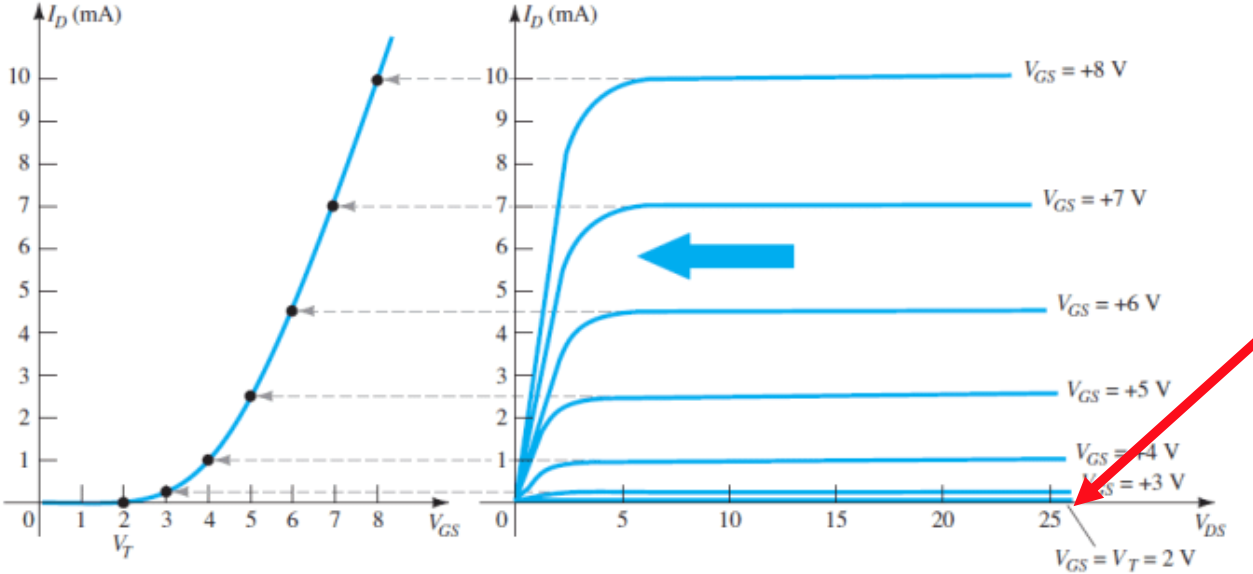
\includegraphics[scale=0.39,angle=0]{n_mos_cutoff.png}
    \caption{Regione di cutoff}
\end{figure}
\\Il grafico di destra ha la tensione $V_{ds}$ sull'asse \textit{x} e la corrente di drain $I_{d}$ sull'asse \textit{y} (in condizione statica è anche la corrente di source $I_{s}$). Nel grafico di sinistra invece, è rappresentato l'andamento della tensione di saturazione $I_{d-sat}$ rispetto alla tensione tra gate e source $V_{gs}$.

\subsection{Lineare}
Nella regione lineare il dispositivo MOS inizia a condurre perché la tensione del gate supera la tensione di soglia:
\begin{equation}
    V_{gs} > V_{t}
\end{equation}
Per ogni tensione di gate si identifica una specifica curva nel grafico di destra. Tutte le curve tendono a salire seguendo un andamento simile; in particolare: più alta è la tensione di gate e più la curva è ripida e alta. Con correnti di drain ragionevolmente basse, cioè
\begin{equation}
    I_{d} < I_{d-sat}
\end{equation}
ci si trova a lavorare in una regione prossima all'asse \textit{y} con tensioni $V_{gs}$ comprese tra $0\,V$ e circa $5\,V$. In questa regione il dispositivo ha un andamento \textit{lineare} con un comportamento che ricorda quello di una \textit{resistenza}; ovvero la corrente $I_{d}$ è \textit{direttamente proporzionale} alla tensione $V_{ds}$ con costante di proporzionalità chiamata \textbf{resistenza di canale} il cui valore è specificato all'interno del datasheet del dispositivo MOS. Ovviamente, la resistenza di canale è inversamente proporzionale, secondo una qualche legge, alla tensione di gate. Non a caso, a valori alti di $V_{gs}$ corrispondono curve più rapide che rappresentano resistenza basse.

Superato un certo valore massimo di corrente $I_{d-sat}$, le curve tendono a diventare parallele all'asse x fermandosi su certo valore per la corrente di drain $I_{d}$.
\begin{figure}[h]
    \centering
    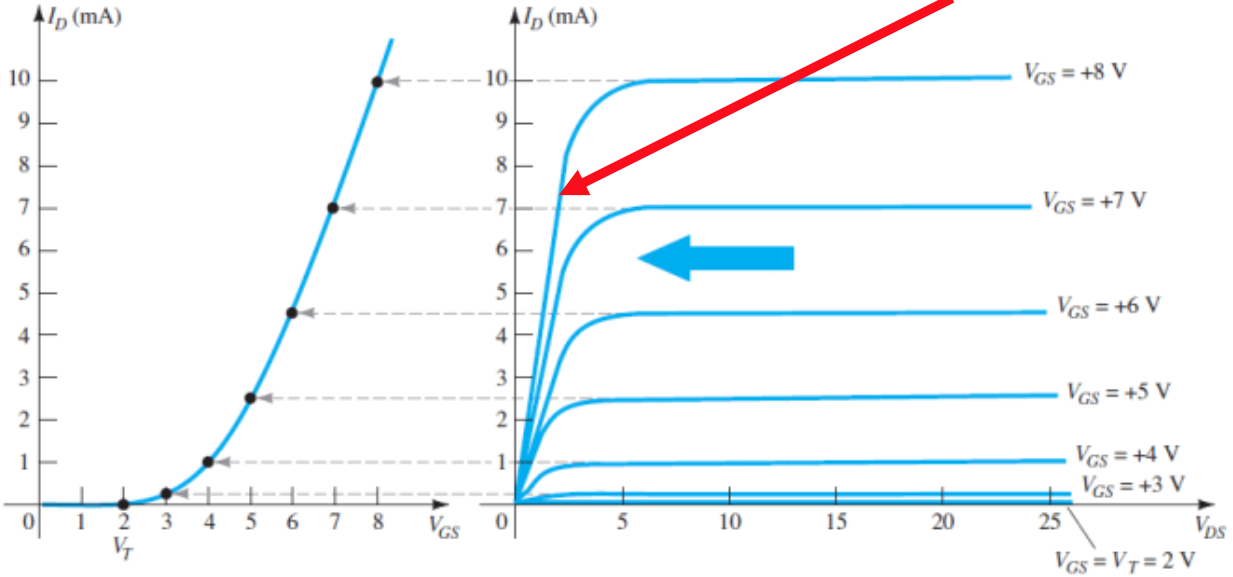
\includegraphics[scale=0.39,angle=0]{n_mos_lineare.png}
    \caption{Regione lineare}
\end{figure}

\subsection{Saturazione}
Questa situazione si verifica nel momento in cui la tensione di gate $V_{gs}$ ha superato la tensione di soglia e, per un qualsiasi valore della tensione di drain $V_{ds}$ maggiore di un certo valore, la corrente di drain $I_{d}$ non aumenta più ma si ferma al valore di saturazione $I_{d-sat}$, cioè
\begin{equation}
    I_{d} = I_{d-sat}
\end{equation}

Di fatto, il dispositivo si comporta come un \textbf{generatore costante di corrente comandato in tensione}; dalla tensione di gate $V_{gs}$. Maggiore è la tensione di gate e maggiore è la corrente di saturazione.
\begin{figure}[h]
    \centering
    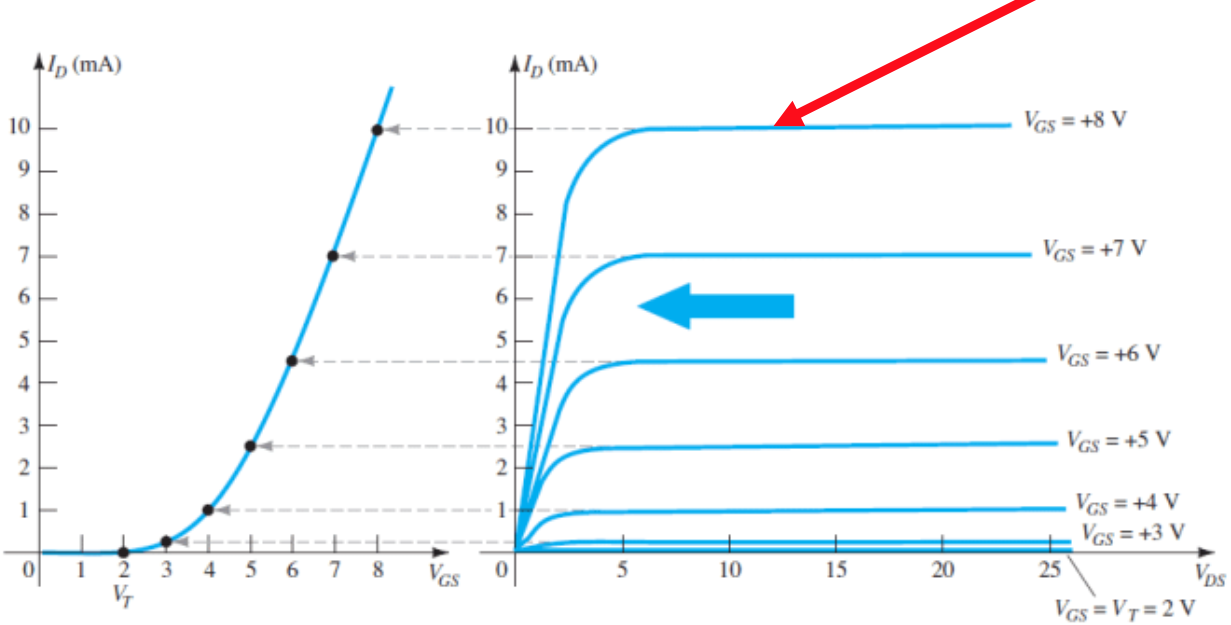
\includegraphics[scale=0.37,angle=0]{n_mos_saturazione.png}
    \caption{Regione di saturazione}
\end{figure}
\subsection{Confronto con il BJT}
La regione di saturazione del BJT è quella regione che corrisponde alla regione lineare di un MOS. Al contrario, la regione attiva diretta (anche chiamata regione lineare) del BJT corrisponde alla regione di saturazione del MOS. Nel caso del MOSFET si parla di saturazione in riferimento alla sua capacità di far passare corrente: sfruttando la tensione di gate $V_{gs}$ sono stati inseriti un certo numero di portatori ma se la differenza di potenziale $V_{ds}$ viene aumentata molto i portatori vengono tutti strappati dal canale che di fatto viene chiuso perché gli vengono tolti gli elettroni di conduzione. Il drain ha tensione positiva che può essere maggiore della tensione di gate, quindi lavora nel verso opposto a come lavora il source cioè, data una certa tensione $V_{gs}$ il source immette elettroni di conduzione mentre il drain, che è a tensione positiva, li toglie quando la sua tensione è maggiore di zero.

\section{Corrente}
Esiste una relazione ben precisa tra le tensioni di gate e drain e la corrente di drain che è definita tramite un'equazione di secondo grado chiamata \textbf{equazione del MOSFET}:
\begin{equation}
    I_{d} = K\,[2(V_{gs} - V_{t})V_{ds} - V_{ds}^2]
\end{equation}
È una \textit{parabola} in $V_{ds}$ con concavità rivolta verso il basso e con coefficiente lineare $2K(V_{gs} - V_{t})$ legato alla tensione di gate. Questa equazione è valida per $V_{gs} > V_{t}$, corrispondente alla regione lineare del dispositivo, e solo fino al \textit{vertice} della parabola che corrisponde al valore massimo di $I_{d}$, cioè al valore di saturazione $I_{d-sat}$. Non a caso se $V_{gs} < V_{t}$ ci si trova nella regione di cutoff del MOS in cui la corrente di drain è nulla e il dispositivo è spento. Il valore di saturazione è definito come:
\begin{equation}
    I_{d-sat} = K(V_{gs} - V_{t})^2
    \label{id_sat}
\end{equation}
che, come si nota nel grafico di sinistra nelle tre foto precedenti, ha un andamento \textit{parabolico} a partire dalla tensione di soglia $V_t$ mentre è \textit{nulla} per $V_{gs} < V_{t}$. L'ascissa del vertice della parabola corrisponde al punto in cui $V_{ds} = V_{gs} - V_{t}$. Dunque nel grafico che ha per ordinata la corrente di drain $I_{d}$ (quello a destra) il vertice della parabola ha ascissa $V_{ds} + V_{t}$ e coordinata $K(V_{gs} - V_{t})^2$.

Per tutte le tensioni $V_{ds} \geq V_{gs} - V_{t}$ ci si trova in saturazione: la corrente $I_{d}$ è costante identicamente pari alla corrente di saturazione $I_{d-sat}$ definita tramite la \eqref{id_sat}. Riassumendo:
\begin{equation*}
I_{d} = \left\{
\begin{array}{ll}
0 &\text{se } V_{gs} < V_{t}\\
K\,[2(V_{gs} - V_{t})V_{ds} - V_{ds}^2] &\text{se } V_{gs} > V_{t} \text{ e } V_{gs} < V_{ds} + V_{t}\\
K(V_{gs} - V_{t})^2 & \text{se } V_{ds} \geq V_{gs} - V_{t} 
\end{array}\right.
\end{equation*}
L'andamento di $I_{d}$ è esattamente quello rappresentato dalle curve nel grafico di destra nelle tre figure precedenti. Questi grafici sono disponibili all'interno del datasheet del dispositivo.

Queste curve variano al variare del parametro $V_{gs} - V_{t}$ che di fatto controlla il valore massimo di corrente che si può raggiungere e il punto in cui è possibile raggiungerlo. È questo il motivo per cui si dice che un N-MOS è un dispositivo controllato in tensione: perché il suo funzionamento è dettato dal parametro $V_{gs} - V_{t}$ che funge da variabile di controllo tramite la quale è possibile definire la corrente $I_{d}$ al variare della tensione $V_{ds}$.

La costante \textit{K} è definita secondo l'equazione:
\begin{equation}
    K = \frac{1}{2}\mu C_{ox}\frac{W}{L}
\end{equation}
Dipende dalla mobilità dei portatori $\mu$ e dai parametri geometrici del dispositivo \textit{W} e \textit{L} che sono rispettivamente la larghezza e la lunghezza del canale, entrambe controllate dal gate.
È \textit{direttamente proporzionale} alla mobilità dei portatori $\mu$ che, nel caso di un N-MOS, corrisponde alla mobilità degli elettroni mentre in un P-MOS corrisponde a quella delle lacune.
Per definizione, tanto più largo è il canale e tanto maggiore sarà \textit{K}, cioè tanto maggiore sarà la corrente che potrà passare nel canale. Viceversa, tanto più lungo è il canale e tanto minore sarà \textit{K} perché i portatori dovranno spostarsi per un tratto più lungo impiegando quindi uno sforzo maggiore (il canale può essere visto come una resistenza). A parità di condizioni, confrontando il K di un MOS a canale n e di uno a canale p, si ha che: \begin{equation*}
    K_{b} \approx 2K_{p}
\end{equation*}

\section{P-MOS}
Anche chiamato \textbf{mosfet a canale p}, è il dispositivo \textit{complementare} ad un N-MOS. Il canale di un P-MOS sarà quindi caratterizzato da lacune e non più da elettroni. Dal punto di vista circuitale è analogo ala transistor di tipo \textit{pnp}.
\begin{figure}[h]
    \centering
    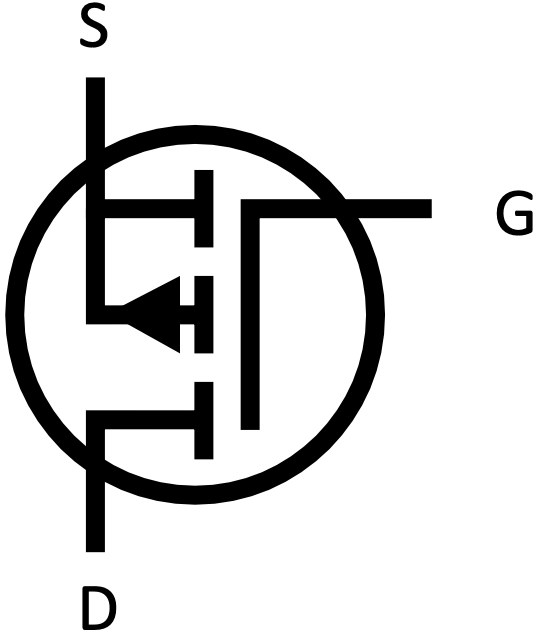
\includegraphics[scale=0.35,angle=0]{p_mos_simbolo.png}
    \caption{Simbolo circuitale del P-MOS}
\end{figure}
\\Per quanto riguarda le tensioni:
\begin{itemize}
    \item[$V_{sd}$]: la tensione tra drain e source. Il source si suppone essere sempre \textit{positivo} mentre il drain si suppone essere sicuramente \textit{negativo} rispetto al source
    \item[$V_{gs}$]: la tensione tra gate e source. Il gate è \textit{negativo} rispetto al source
    \item[$V_{dg}$]: la tensione tra drain e gate
\end{itemize}
Le tre correnti sono così definite:
\begin{itemize}
    \item[$I_{s}$]: la corrente del source, si prende \textit{positiva} quando è \textit{entrante} nel dispositivo
    \item[$I_{d}$]: la corrente del drain, si prende \textit{positiva} quando è \textit{uscente} dal dispositivo
    \item[$I_{g}$]: la corrente del gate
\end{itemize}
Applicando inizialmente una tensione di gate $V_{gs}$ (negativa per definizione) minore, cioè \textit{più negativa}, di una tensione di soglia negativa $V_{gs} < - |V_{t}|$, si crea una \textbf{regione di svuotamento} (come in figura \ref{svuotamento}) del tutto complementare a quella che si forma all'interno di un N-MOS. Questa complementarietà è dovuta al fatto che dentro un P-MOS è presente una vasta zona in silicio drogato di tipo n sulla quale sono presenti due piccole zone drogate p+ in corrispondenza di source e drain. La zona a drogaggio n è poi in contatto con uno strato di ossido isolante sopra il quale è collocato il gate in metallo. La presenza della zona drogata n (e non p come in un N-MOS) comporta che dentro di essa, in corrispondenza della regione di svuotamento, si vanno ad accumulare delle lacune che formano una carica positiva nel semiconduttore mentre se ne crea una negativa nel gate.
\begin{figure}[h]
    \centering
    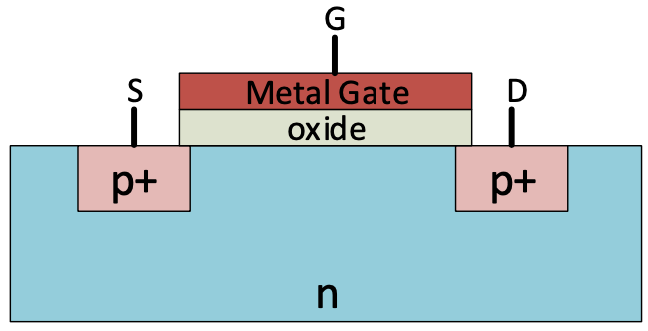
\includegraphics[scale=0.45,angle=0]{p_mos_struttura.png}
    \caption{Struttura di un P-MOS}
\end{figure}

Diminuendo ancora di più la tensione di gate, quando sarà sufficientemente negativa sarà in grado di attrarre ulteriori lacune dalle due zone p+ adiacenti, queste lacune si disporranno al di sotto della regione di svuotamento e, essendo lacune libere, potranno fungere da portatori di carica. Potrà quindi scorrere corrente tra i terminali drain e source. Tuttavia in questa corrente saranno le lacune a muoversi ma esse hanno una mobilità che è circa la metà di quella degli elettroni (come già detto parlando dei BJT) e questo fa sì che le prestazioni di un P-MOS siano generalmente \textit{minori} rispetto a quelle di un N-MOS. A parità di funzionamento, il P-MOS porta metà corrente rispetto a quella portata da un N-MOS.\\

Riassumendo, per entrambi le tipologie di MOSFET, si quella a canale n che quella a canale p, si identificano tre regioni operative:
\begin{description}
    \item[Cutoff] non c'è conduzione tra source e drain perché $|V_{gs}| < |V_{t}|$ implica che non può scorrere corrente all'interno del canale
    \item[Regione lineare] in questo caso $|V_{gs}| > |V_{t}|$ e $|I_{d}| < |I_{d-sat}|$. Finché non si raggiunge la corrente limite $I_{d-sat}$ dettata dalla tensione $V_{gs}$, si ha un andamento inizialmente lineare e poi più marcatamente parabolico della corrente. In queste condizioni il dispositivo si comporta come un resistore controllato in tensione
    \item[Saturazione] in questo caso $|I_{d}| = |I_{d-sat}|$. Si è raggiunto il valore limite della corrente definito tramite l'equazione \eqref{id_sat}. La corrente non cresce più, quindi l'uscita è costante indipendentemente dalla tensione applicata sul drain. In queste condizioni il dispositivo si comporta come un generatore di corrente costante controllato in tensione
\end{description}

\section{N-MOS reale}
Nella realtà fisica, un dispositivo N-MOS è \textbf{asimmetrico} per costruzione. In particolare, la metallizzazione del source tramite l'impiego dell'alluminio mette in \textit{cortocircuito} anche una parte del semiconduttore drogato p, quindi il source e il \textbf{body} del diodo sono collegati insieme: una certa zona del semiconduttore di tipo p (la parte bassa della zona p riportata in figura \ref{struttura_nmos}) ha lo stesso potenziale del source. Questo comporta che si viene a creare un diodo, chiamato \textbf{body diode}, tra il drain e il source messo in cortocircuito con il semiconduttore di tipo p. Questo diodo è presente nella maggior parte dei MOSFET. È questo il motivo per cui, in condizioni normali, per avere il comportamento finora descritto, si deve avere il potenziale di drain \textit{maggiore} di quello di source perché se così non fosse il diodo body si polarizzerebbe \textit{direttamente} e scorrerebbe corrente dal source al drain senza nessun controllo da parte del gate, cioè indipendentemente dalla tensione di gate.
\begin{figure}[h]
    \centering
    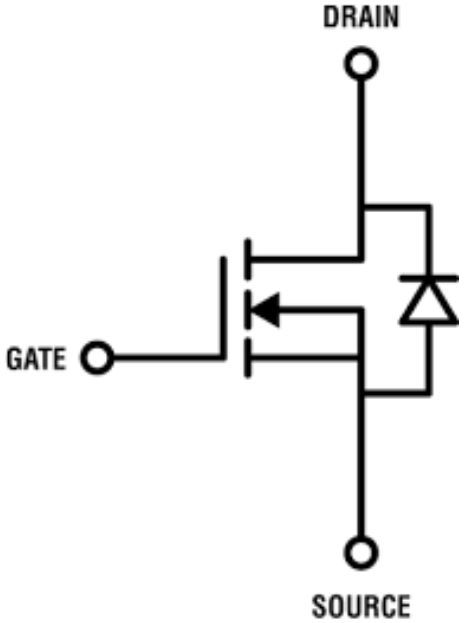
\includegraphics[scale=0.4,angle=0]{n_mos_reale.png}
    \caption{Body diode}
\end{figure}
\\Al contrario, in un MOS a canale p si deve fare in modo che il drain sia sempre più \textit{negativo} del source.

Indipendentemente dalla tipologia di MOS, come nel caso dei diodi e transistor, ci sono delle limitazioni riguardo le tensioni che possono essere applicate al drain e se queste non sono rispettate il dispositivo si romperà. Questo perché se la tensione applicata al drain è troppo elevata (maggiore della \textbf{tensione di breakdown}), il campo elettrico che si crea tra drain e source è così elevato da perforare il canale. In questo scenario le curve di corrente $I_{d}$ impennano rapidamente verso l'alto e questo di fatto rappresenta la rottura del dispositivo.

\section{Impiego dei MOS}
Normalmente si utilizzano sia i P-MOS che gli N-MOS. Nelle logiche C-MOS sono presenti le due tipologie accompagnate da alcuni accorgimenti per garantire che entrambe abbiano la stessa prestazione. Nell'elettronica di potenza, in cui si utilizzano questi dispositivi come interruttori o per svolgere compiti gravosi in termini di potenza richiesta, si cerca di sfruttare al meglio gli N-MOS grazie alle loro prestazioni nettamente migliori in modo del tutto analogo al contesto dei BJT in cui si tendono a preferire quelli di tipo npn. 
\begin{figure}[h]
    \centering
    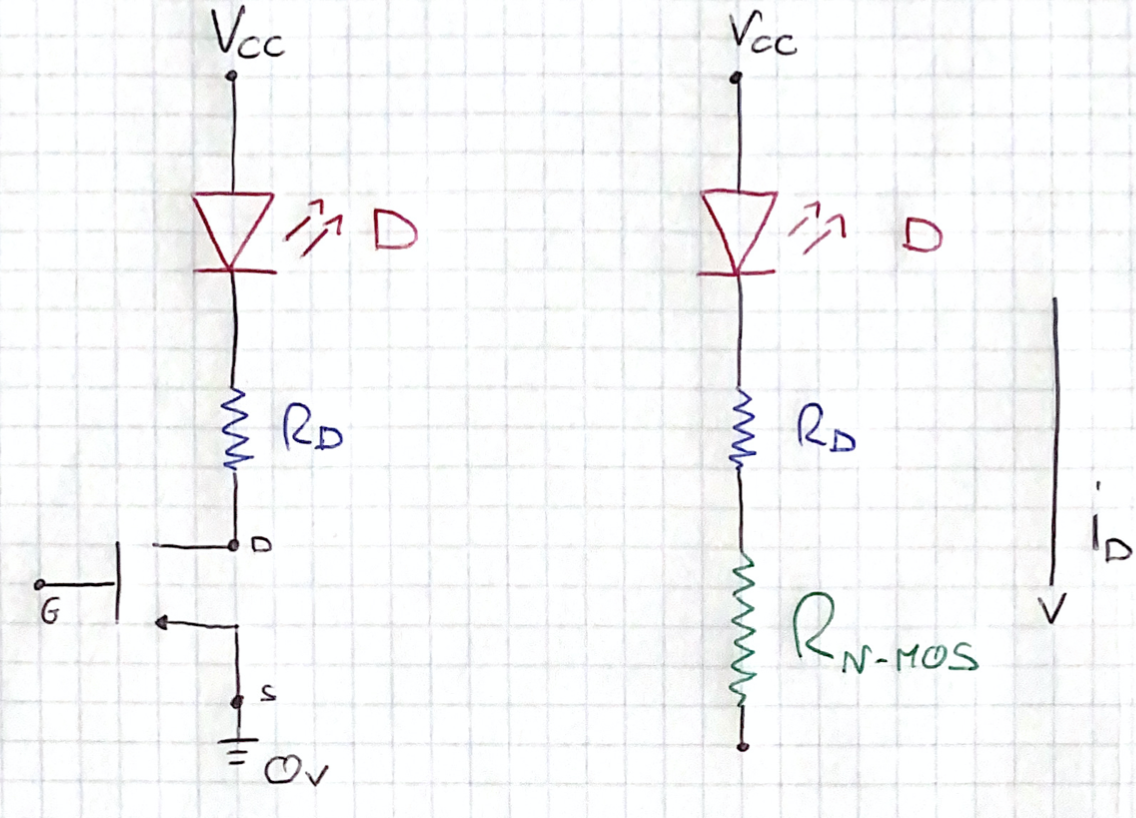
\includegraphics[scale=0.35,angle=0]{mos_interruttore.png}
    \caption{Body diode}
\end{figure}
\\Nel seguente circuito, il MOS a canale n viene utilizzato come interruttore per gestire il carico soggetto ad una tensione $V_{cc}$ e composto da una resistenza $R_{d}$ e da un LED $D$ da accendere. Il carico è collegato al drain, il source viene messo a $0\,V$ mentre il gain riceve un segnale in ingresso. Quando la tensione applicata sul gate è maggiore della tensione di soglia $V_{t}$, si attiverà il canale del gate tra source e drain trasformandolo in una opportuna resistenza. Se per esempio il gate è soggetto ad una tensione di $5\,V$ e la tensione di soglia del MOS è $V_{t} = 2\,V$, si può sostituire il MOS con la corrispettiva \textit{resistenza di canale} $R_{n-mos}$ il cui valore è fornito dal datasheet del dispositivo. A questo punto si deve determinare la corrente che scorre nel circuito e poi controllare che valga $I_{d} < I_{d-sat}$, se è vero significa che il MOS si sta effettivamente comportando come una resistenza, come se fosse un interruttore. Se invece $I_{d} > I_{d-sat}$, l'ipotesi di resistenza di canale decade e la corrente sarà limitata alla corrente di saturazione $I_{d} = I_{d-sat}$.

\chapter{Circuiti logici digitali}
I \textbf{circuiti logici digitali} sono tutti quei circuiti in cui l'informazione è \textbf{quantizzata} in soli due possibili livelli chiamati \textbf{stati digitali}: alto e basso, vero o falso, 0 o 1. Alla base di tutto c'è l'\textbf{algebra di Boole}, l'aritmetica binaria. L'impiego di solo due livelli possibili permette di semplificare il trasferimento dell'informazione da un dispositivo all'altro perché il ricevente è in grado di discriminare facilmente i due stati.

\section{Operatori booleani}
Per poter effettuare delle operazioni logiche si sfrutta l'algebra booleana tramite la quale si definiscono gli \textbf{operatori booleani}.
\begin{itemize}
    \item\textbf{AND}: indicato con una linea sopra l'operando che deve essere negato.
    \begin{figure}[h]
    \centering
    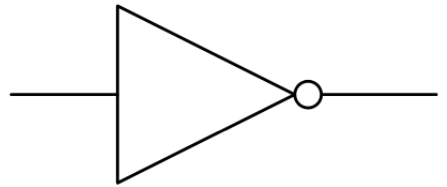
\includegraphics[scale=0.5,angle=0]{logica_not.png}
    \caption{Simbolo circuitale del NOT}
    \end{figure}
    \\La sua tabella di verità è la seguente:
    \begin{table}[h]
        \centering
        \begin{tabular}{c|c}
        \em A & $\overline{A}$\\\hline
        0 &1\\
        1 &0
        \end{tabular}
        \caption{Tabella di verità del NOT}
    \end{table}
    \item\textbf{AND}: indicato come il prodotto tra i due operandi, è la moltiplicazione binaria.
    \begin{figure}[h]
        \centering
        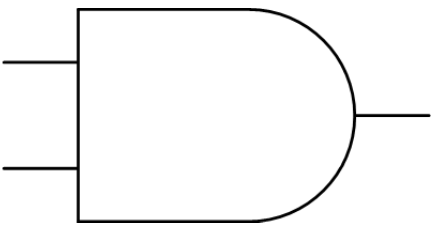
\includegraphics[scale=0.5,angle=0]{logica_and.png}
        \caption{Simbolo circuitale dell'AND}
    \end{figure}
    \\L'uscita dell'AND è vera solo se tutti gli ingressi sono veri. La sua tabella di verità è:
    \begin{table}[ht]
        \centering
        \begin{tabular}{c c |c}
        \em A &\em B &$A \cdot B$\\\hline
        0 &0 &0\\
        0 &1 &0\\
        1 &0 &0\\
        1 &1 &1
        \end{tabular}
        \caption{Tabella di verità dell' AND}
    \end{table}
    \item\textbf{OR}: indicato come la somma tra i due operandi, è la somma logica.
    \begin{figure}[h]
        \centering
        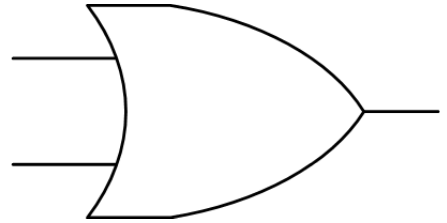
\includegraphics[scale=0.5,angle=0]{logica_or.png}
        \caption{Simbolo circuitale dell' OR}
    \end{figure}
    \\L'uscita dell'AND è vera se almeno uno degli ingressi è vero. La sua tabella di verità è la seguente:
    \begin{table}[h]
        \centering
        \begin{tabular}{c c |c}
        \em A &\em B &$A + B$\\\hline
        0 &0 &0\\
        0 &1 &1\\
        1 &0 &1\\
        1 &1 &1
        \end{tabular}
        \caption{Tabella di verità dell' OR}
    \end{table}
\end{itemize}
\subsection{Leggi di De Morgan}
Le \textbf{leggi di De Morgan} sono leggi relative alla logica booleana utilizzate per l'analisi di circuiti logici e stabiliscono relazioni di equivalenza tra gli operatori logici AND e OR. I due teoremi sono duali tra loro:
\begin{itemize}
    \item Riscrivendo l'operazione di disgiunzione logica come
    \begin{equation*}
        A + B = \overline{\overline{A} \cdot \overline{B}}
    \end{equation*}
    si ricava la prima legge di De Morgan secondo la quale:
    \begin{equation}
        \overline{A + B} = \overline{A} \cdot \overline{B}
    \end{equation}
    dove $\overline{A + B}$ è la negazione dell'operazione logica OR che viene chiamata \textbf{NOR}.
    \item Considerando la congiunzione logica come
    \begin{equation*}
        A \cdot B = \overline{\overline{A} + \overline{B}}
    \end{equation*}
    si ricava la seconda legge di De Morgan, duale alle prima:
    \begin{equation}
        \overline{A \cdot B} = \overline{A} + \overline{B}
    \end{equation}
    con $\overline{A \cdot B}$ la negazione logica dell'AND chiamata \textbf{NAND}.
\end{itemize}

\subsection{Universalità}
Utilizzando i tre operatori logici AND, OR e NOT è possibile descrivere tutte le funzioni logiche per un qualsiasi numero di ingressi e uscite. Questo perché tramite la formule di De Morgan si può passare da una forma logica di somma ad una di prodotto e viceversa e questo permette di scambiare tra di loro le porte logiche. Una qualsiasi funzione booleana può essere espressa come prodotto di somme o come somma di prodotti e negazioni.

In particolare, per sintetizzare una qualsiasi funzione logica ci sono essenzialmente tre possibili gruppi di porte logiche da utilizzare:
\begin{enumerate}
    \item La porta NOT e almeno una porta tra AND, OR, NAND e NOR
    \item La sola porta NOR questo perché mettendo in cortocircuito i due terminali di ingresso alla porta si ottiene una porta NOT
    \item La sola porta NAND per lo stesso motivo detto sopra
\end{enumerate}
Se per esempio si considera la porta NOR, la sua tabella di verità è la seguente:
\begin{table}[ht]
        \centering
        \begin{tabular}{c c |c}
        \em A &\em B &$\overline{A + B}$\\\hline
        0 &0 &1\\
        0 &1 &0\\
        1 &0 &0\\
        1 &1 &0
        \end{tabular}
\end{table}
\\Imponendo ora il corto tra i due ingressi \textit{A} e \textit{B} deve valere il vincolo aggiuntivo $A = B$ quindi si considerano solo la prima e l'ultima riga della tabella precedente:
\begin{table}[ht]
        \centering
        \begin{tabular}{c c |c}
        \em A &\em B &$\overline{A + B}$\\\hline
        0 &0 &1\\
        1 &1 &0
        \end{tabular}
\end{table}
\\che non è altro che la tabella di verità della NOT.

Quindi per potere sintetizzare ogni possibile funzione logica, cioè ogni possibile dispositivo digitale, è sufficiente essere in grado di sintetizzare una funzione tra NAND e NOR. Tutto il resto si ottiene costruendo circuiti logici sempre più complessi sopra il dispositivo inizialmente costruito che sintetizza una NAND o una NOR.

\section{Parametri delle famiglie logiche}
Quando si parla di \textbf{famiglia logica} si intende un certo insieme di dispositivi che sfruttano la medesima tecnologia, per esempio i transistor bipolari oppure i MOSFET complementari.

All'interno di una famiglia logica ci si può aspettare che i dispositivi comunichino tra loro mediante segnali logici (alto o basso) che, nel mondo elettronico, si traducono in \textbf{tensioni}. Si distinguerà dunque una tensione alta da una tensione bassa che corrisponderà ad uno dei due livelli logici: alto e basso, vero e falso.

Il dispositivo ricevente dovrà essere in grado di discriminare il segnale in ingresso tra i due possibili livelli logici. Per farlo, la tensione deve poter essere discriminata e questo lo si può fare senza imprecisioni se si dispone di un certo margine sulla decisione.

Il fatto che i dispositivi appartenenti alla medesima famiglia logica comunicano tra loro implica che questi dispositivi hanno degli ingressi e delle uscite. Inoltre ci sarà una certa corrente che scorre nei dispositivi in relazione ala fatto che su di essi vieni applicata una tensione in ingresso e sua volta definiscono una tensione di uscita.

\subsection{Parametrici statici}
I \textbf{parametri} delle famiglie logiche si distinguono in \textbf{parametri statici} e in \textbf{parametri dinamici}. I parametrici \textit{statici} sono analizzati quando non ci sono commutazioni di stati logici, cioè quando l'uscita o l'ingresso sono fermi, e sono i seguenti:
\begin{description}
    \item[Tensioni soglia di ingresso] $V_{iH}$ e $V_{iL}$ entrambi definiti su base statistica
    \item[Tensioni soglia di uscita] anche dette livelli logici, sono $V_{oH}$ e $V_{oL}$
    \item[Corrente assorbita in ingresso] $I_{iH}$ e $I_{iL}$
    \item[Margine di rumore] legato a quanto è robusta la famiglia logica
    \item[Fan-out] il numero di porte logiche che si possono guidare con una sola uscita, cioè quanti ingressi possono essere collegati ad un'uscita senza che smetta di funzionare il circuito 
    \item[Consumo statico di potenza] quanto consuma la porta logica in condizione statica
\end{description}
Nello specifico:
\begin{itemize}
    \item[$V_{iH}$]: è un \textbf{parametro di ingresso} che definisce la \textit{minima} tensione di ingresso, applicata all'ingresso della porta logica, che è determinata come valore logico \textit{alto}. Quindi ogni tensione $V \geq V_{iH}$ è interpretata come lo stato logico alto, vero
    \item[$V_{iL}$]: anche questo è un parametro di ingresso che definisce la \textit{massima} tensione di ingresso che è determinata come valore logico \textit{basso}. Ogni tensione $V \leq V_{iL}$ è interpretata come lo stato logico basso, falso.
    
    Deve valere
    \begin{equation}
        V_{iH} > V_{iL}
    \label{soglia_ingresso}
    \end{equation}
    perché se si intersecassero esisterebbero delle tensioni per cui il livello logico risulterebbe \textit{indeterminato}, ovvero non si potrebbe distinguere tra alto e basso. Inoltre, non solo deve valere la \eqref{soglia_ingresso} ma l'intervallo che separa $V_{iL}$ da $V_{iH}$ deve essere il più \textit{piccolo} possibile. Il caso ideale è che le due tensioni coincidano in modo che ogni tensione maggiore della tensione soglia $V_{soglia} = V_{iL} = V_{iH}$ venga interpretata come vero e ogni tensione minore venga interpretata come falso. Tuttavia il caso ideale non è realizzabile perché il valore della tensione di soglia che discrimina tra vero e falso sarebbe destinato a cambiare nel tempo e nello spazio dei circuiti prodotti poiché è un valore determinato da una serie di aspetti dello specifico circuito quali: la tensione di alimentazione, la temperatura di funzionamento, l'invecchiamento del circuito e la variabilità di produzione. Per evitare questa variabilità della tensione soglia è preferibile definire statisticamente un intervallo di tensioni che non corrispondono a nessun livello logico. L'estensione di questo intervallo dipende dalla variabilità di produzione del circuito. Comunque, ogni porta logica nella sua singolarità avrà un proprio valore di soglia con il quale discriminerà tra livello logico alto e basso
    \item[$V_{oH}$]: è un \textbf{parametro di uscita} che definisce la \textit{minima} tensione di uscita che è garantita quando il valore logico dell'uscita è \textit{alto}. Questo significa che per avere il livello logico alto nell'uscita, al variare di tutti i parametri citati in precedenza, la tensione di uscita dovrà essere \textit{almeno} pari a $V_{oH}$
    \item[$V_{oL}$]: il secondo parametro di uscita che definisce la \textit{massima} tensione di uscita che è garantita quando il valore logico dell'uscita è \textit{basso}. Dunque, statisticamente, quando si presenta in uscita il livello logico basso la tensione di uscita dovrà essere \textit{al massimo} $V_{oL}$. Anche in questo caso deve valere
    \begin{equation}
        V_{oH} > V_{oL}
    \end{equation}
    e si vorrebbe $V_{oH}$ la più grande possibile e $V_{oL}$ la più bassa possibile per non avere incertezze nelle discriminazione del livello logico corrispondente
    \item[$I_{iH}$]: è la corrente in ingresso alla porta logica quando il livello logico ricevuto è \textit{alto}. È quindi la corrente entrante determinata dalla tensione $V_{oH}$ applicata sull'uscita della porta logica da cui proviene il segnalo logico ricevuto
    \item[$I_{iL}$]: è la corrente che passa dall'ingresso della porta logica quando il livello logico ricevuto è \textit{basso}. In realtà, per tensioni basse in ingresso si suppone che la corrente abbia un verso\textit{opposto}, ovvero uscente dall'ingresso della porta logica che ha ricevuto il segnale.
    
    Questi due parametri di corrente sono importanti perché quando si costruisce un circuito logico si utilizzano sia BJT che MOS e, utilizzandoli come dispositivo di uscita con un certo numero di ingressi, la corrente in ingresso $I_{iH}$ o $I_{iL}$ sarà moltiplicata per il numero di ingressi connessi insieme. Dunque dovrà esserci un limite alle porte logiche connesse alla medesima uscita per non ottenere una corrente troppo elevata che manderebbe il transistor in saturazione o il MOS in regione lineare
\end{itemize}
Da tutti questi parametri si ricavano i cosiddetti \textbf{parametri derivati} che sono il \textit{margine di rumore}, indicato con \textit{NM}, il \textit{fan-out} e il \textit{consumo statico di potenza} indicato con \textit{P}:
\begin{itemize}
    \item[\textit{NM}]: quanto è resistente la famiglia logica a piccole imperfezioni (ovvero il \textbf{rumore elettrico}) dell'interconnessione tra ingresso e uscita di una porta logica e la successiva. È definito come:
    \begin{equation}
        \textit{NM} = min(\textit{NM}_{L},\, \textit{NM}_{H})
    \end{equation}
    dove i  due valori iniziali $\textit{NM}_{L}$ e $\textit{NM}_{H}$ sono chiamati rispettivamente \textbf{margine di rumore basso} e \textbf{margine di rumore alto}, e sono definiti come:
    \begin{equation*}
        \textit{NM}_{L} = V_{iL} - V_{oL} \text{ \, \, }  \textit{NM}_{H} = V_{oH} - V_{iH}
    \end{equation*}
    Sicuramente $\textit{NM}_{H} > 0$ perché non è altro che la differenza tra il minimo garantito in uscita e il minimo richiesto in ingresso (con $V_{iH} < V_{oH}$) e rappresenta il margine affinché non ci siano problemi di false commutazioni logiche; dunque è tutto il rumore elettrico che si può tollerare senza commettere un errore di valutazione del livello logico. Analogamente, $\textit{NM}_{L} > 0$ perché $V_{iL} > V_{oL}$ e anche in questo caso rappresenta il rumore elettrico che si può tollerare senza sbagliare la stima della funzione logica. Si tende sempre a cercare di bilanciare $\textit{NM}_{L}$ e $\textit{NM}_{H}$ in modo che non siano troppo distanti. Normalmente succede che le famiglie logiche bipolari (quelle costruite utilizzando BJT) sono un po' sbilanciate e quindi \textit{NM} ne risente. Al contrario, le famiglie logiche C-MOS sono costruite appositamente per essere simmetriche e quindi i due margini di rumore sono uguali e questo massimizza il margine di rumore generico
    \item[Fan-out]: il massimo numero di ingressi che si possono collegare ad una singola uscita in modo da garantire il mantenimento del corretto risultato logico in uscita. È un numero pre-determinato perché la porta logica può assorbire una certa corrente in ingresso che deve essere sostenuta la porta logica di uscita. Dipende da quanta corrente l' uscita è in grado di guidare verso quanta corrente viene assorbita da ogni porta logica. Più grande è il fan-out e maggiore sarà il numero di porte in input che possono essere collegate insieme
    \item[P]: la potenza dissipata dalla singola cella logica in condizioni \textit{statiche}, cioè quando la cella è ferma con la sua uscita alta o bassa. Poiché mediamente e statisticamente è vero che i livelli logici alto e basso, vero e falso, hanno la stessa probabilità, la potenza statica viene definita come:
    \begin{equation}
        P = \frac{P_{H} + P_{L}}{2}
    \end{equation}
    ovvero è la potenza media dei due casi. Questo valore può essere usato anche per stimare quante celle logiche possono essere raggruppate con quella specifica tecnologia all'interno del circuito integrato. Tanto più bassa è la potenza statica \textit{P} e tante più celle logiche si riusciranno a mettere nel medesimo circuito
\end{itemize}

\subsection{Parametri dinamici}
I \textbf{parametri dinamici} sono tutti quei parametri che si verificano quando c'è un cambiamento dell'ingresso che si traduce sia in un cambiamento dell'uscita della porta logica sia in un cambiamento della configurazione del circuito elettronico che fa sì che si vada a consumare dell'energia durante questa transizione. I più importanti sono i seguenti:
\begin{description}
    \item[Tempo di propagazione] anche detto \textbf{propagation delay}, indica il tempo necessario ad un'informazione che è cambiata in ingresso per arrivare all'uscita. Il segnale elettronico ricevuto in ingresso deve attraversare una serie di circuiti elettrici prima di arrivare all'uscita; il tempo necessario ad attraversarli tutti è proprio il tempo di propagazione. Questo tempo potrebbe essere diverso a seconda che la transizione dell'uscita sia da alto a basso o da basso ad alto perché durante la propagazione potrebbero accadere cose diverse. In relazione a queste due possibilità si definiscono due diversi tempi di propagazione indicati rispettivamente con $t_{p_{HL}}$ e $t_{p_{LH}}$. Si cerca sempre di ridurlo per aumentare la frequenza d'uso dei dispositivi logici e inoltre, se un circuito ha un certo tempo di propagazione dall'ingresso all'uscita, l'ambiente in cui tale circuito è impiegato non può commutare stato ad una frequenza maggiore di quella del circuito perché se lo facesse non riuscirebbe a vedere il cambiamento della porta logica in quanto non è in grado di mostrare in uscita correttamente il suo valore aggiornato 
    \item[Potenza di commutazione] anche chiamata \textbf{switching power} o più correttamente energia di commutazione, indica l'energia consumata quando il circuito commuta da uno stadio logico basso ad uno alto e viceversa. Si è visto che il gate di un MOSFET è un condensatore: per caricarlo si deve inserire della carica al suo interno, quindi si deve inserire della corrente e questo significa mettere dell'energia. Dunque per far cambiare stadio ad un MOSFET ci vuole energia, in particolare serve energia ogni volta che si deve smuovere il potenziale di punti che presentano delle capacità; tutto questo viene riassunto nella potenza di commutazione.
    
    Questo valore è diverso dalla potenza statica \textit{P} perché essa viene definita in condizioni statiche e rappresenta una corrente che scorre continuamente nel circuito. Al contrario, l'energia di commutazione si calcola solo durante la commutazione, è legata a quanto questa energia viene spesa come potenza a seconda di quante volte al secondo il circuito commuta. Dipende quindi dalla \textit{frequenza} con cui commuta il circuito: tante più commuterà al secondo e tanta più energia sarà richiesta: è una potenza che cresce \textit{linearmente} con la frequenza di utilizzo del circuito
    \item[Prodotto ritardo-potenza - DP] è definito come il prodotto tra il tempo di propagazione del circuito ($t_{p_{HL}}$ o $t_{p_{LH}}$) e la potenza dissipata (si può fare sia con quella statica che con quella dinamica). Se si vuole che il circuito commuti velocemente si deve aumentare la potenza consumata e viceversa: tanta meno potenza consuma e tanto più tempo impiegherà per commutare. Cioè che rimane normalmente invariante è il prodotto di queste grandezze 
\end{description}
Per una certa famiglia logica il parametro di riferimento è il prodotto ritardo-potenza in quanto riassume al suo interno il bilancio tra tempo di propagazione e potenza di commutazione consumata.

\chapter{RTL}
La prima famiglia logica esaminata è la \textbf{RTL - Resistor Transistor Logic}, una famiglia ormai non più presente sul mercato basata sull'impiego di sole resistenze e transistors.

\section{NOT}
La porta \textbf{NOT} è la più semplice porta da realizzare perché sono sufficienti due resistenze e un solo transistor. È l'invertitore più semplice da realizzare anche se ha un consumo considerevole. La sua versione basilare in logica RTL è data dal seguente circuito:
\begin{figure}[h]
    \centering
    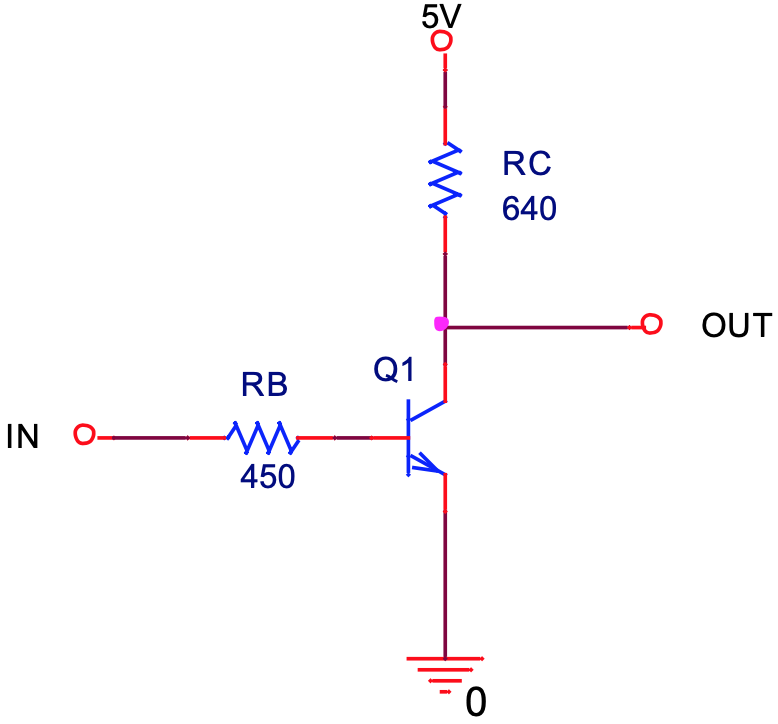
\includegraphics[scale=0.38,angle=0]{rtl_not.png}
    \caption{Struttura del NOT in logica RTL}
\end{figure}
\\Se l'ingresso \textit{IN} è  \textit{basso} (per esempio si applica una tensione in ingresso di $0\,V$) non può scorrere corrente nella base del transistor $Q_1$ che si troverà quindi nella regione di \textit{cutoff}. Essendo il transistor in interdizione, non scorre corrente tra collettore ed emettitore e quindi non scorre corrente nemmeno nella resistenza di collettore $R_c$ se non per alimentare una eventuale uscita. Dunque, in assenza di carico, l'uscita sarà \textit{alta}.

Se invece l'ingresso è \textit{alto}, nella resistenza di base $R_b$ e nella giunzione \textit{pn} tra la base e l'emettitore scorre corrente, questo fa attivare la base del transistor e scorrerà una corrente dal collettore all'emettitore proporzionale al guadagno $h_{fe}$. Dunque l'uscita \textit{OUT} sarà \textit{bassa} poiché scorre corrente nella resistenza di collettore $R_c$ che causa una caduta di potenziale.

\section{NOR}
Rimanendo nel contesto della famiglia logica RTL, la seconda porta logica che nasce più facilmente dopo la porta NOT è la \textbf{NOR}. Le due porte, come accennato nel capitolo precedente, sono sufficienti per poter implementare una qualsiasi funzione logica. La porta NOR è composta da due celle di ingresso entrambe composte da una resistenza di base $R_b$ e un transistor $Q$. Entrambi i collettori sono connessi con la medesima resistenza di collettore $R_c$ ed entrambi gli emettitori sono a terra.
\begin{figure}[h]
    \centering
    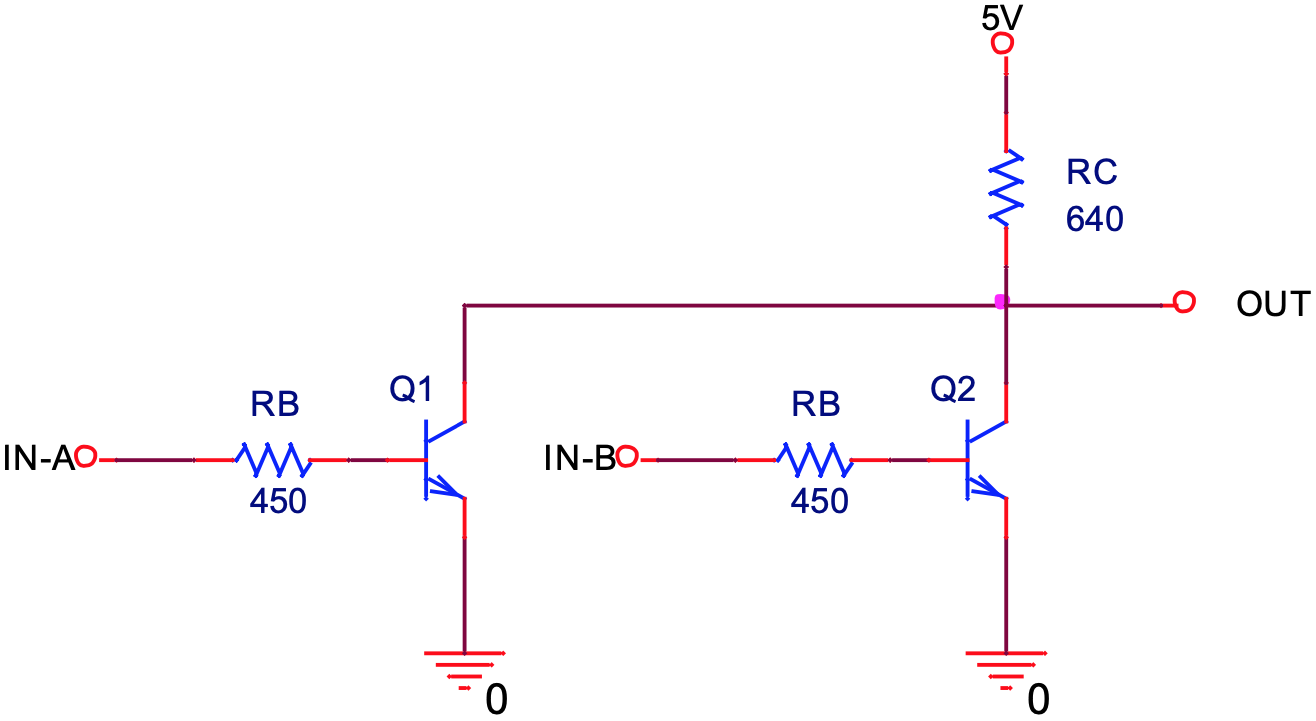
\includegraphics[scale=0.4,angle=0]{rtl_nor.png}
    \caption{Struttura del NOR in logica RTL}
\end{figure}

La corrente che passa attraverso la resistenza di collettore $R_c$ può passare sia attraverso $Q_1$ che $Q_2$, quindi è sufficiente che una delle due celle sia attiva per far scorrere una corrente in $R_{c}$ e avere uscita \textit{OUT bassa} ricalcando così la tabella di verità del NOR. Una generica cella è attiva quando il suo ingresso è \textit{alto} ovvero la tensione in ingresso $V_{in-a}$ e/o $V_{in-b}$ è alta. Se almeno una cella è attiva, nel collettore del suo transistor scorrerà una corrente che farà abbassare il potenziale del collettore facendo scorrere una corrente attraverso il carico $R_c$ e questo abbassamento di potenziale determinerà un'uscita bassa dalla porta logica. Se invece nessuna delle due celle è attiva non passa corrente quindi l'uscita rimarrà \textit{alta}.

Poiché le due celle di ingresso sono in parallelo la corrente può scorre in entrambe oppure in una delle due, in ogni caso la corrente delle due celle si somma e va a formare la corrente che scorre della resistenza di collettore.

\section{Parametri della porta NOT}
Quando si descrive una famiglia logica si devono fornire i valori di tutti i suoi parametri statici e dinamici. Per definire i parametri si deve procedere analiticamente osservando come varia la tensione di uscita del circuito al variare della tensione di ingresso.

Come si nota dal grafico in figura \ref{not_transfer} per ingressi bassi l'uscita è alta mentre per ingressi alti l'uscita è bassa. In particolare, per tensioni di ingresso basse comprese tra $0\,V$ e circa $0,6\,V$ l'uscita è alta, mentre per tensioni alte da circa $0,7\,V$ in poi l'uscita e bassa. È poi presente una \textbf{regione di transizione} per valori di tensione in ingresso compresi tra circa $0,55\,V$ e $0,7\,V$ in cui l'uscita bassa da alta a bassa.

Tendenzialmente si verifica l'effetto porta logica (verificabile anche a livello circuitale) per cui l'uscita della porta tende effettivamente ad avere un andamento logico, ovvero o è solo alta o solo bassa.

Guardando più nel dettaglio la regione di transizione è possibile ricavare informazioni circa la caratteristica della porta logica. Osservando la figura \ref{not_transfer_zoom} si nota che intorno ai $500 - 550\,mV$ (diventando poi più marcata a partire dai $600\,mV$) la curva di tensione, che all'inizio è stabilmente alta, incomincia a scendere. Questo è dovuto al fatto che la giunzione tra la base e l'emettitore del transistor inizia ad accendersi e conseguentemente inizia a scorrere una esigua corrente di base. La giunzione al silicio si considera completamente accesa intorno agli $0,7\,V$, infatti intorno a quel valore di tensione il transistor riceverà così tanta corrente in base che tutta la corrente di collettore che vorrebbe scorrere nel transistor lo porterà in \textit{saturazione} e, dato il valore della resistenza di collettore $R_c$, la corrente che effettivamente scorrerà al suo interno sarà $I_{c} < h_{fe} \cdot I_{d}$ come da definizione di regione di saturazione in un BJT.
\begin{figure}[h]
    \centering
    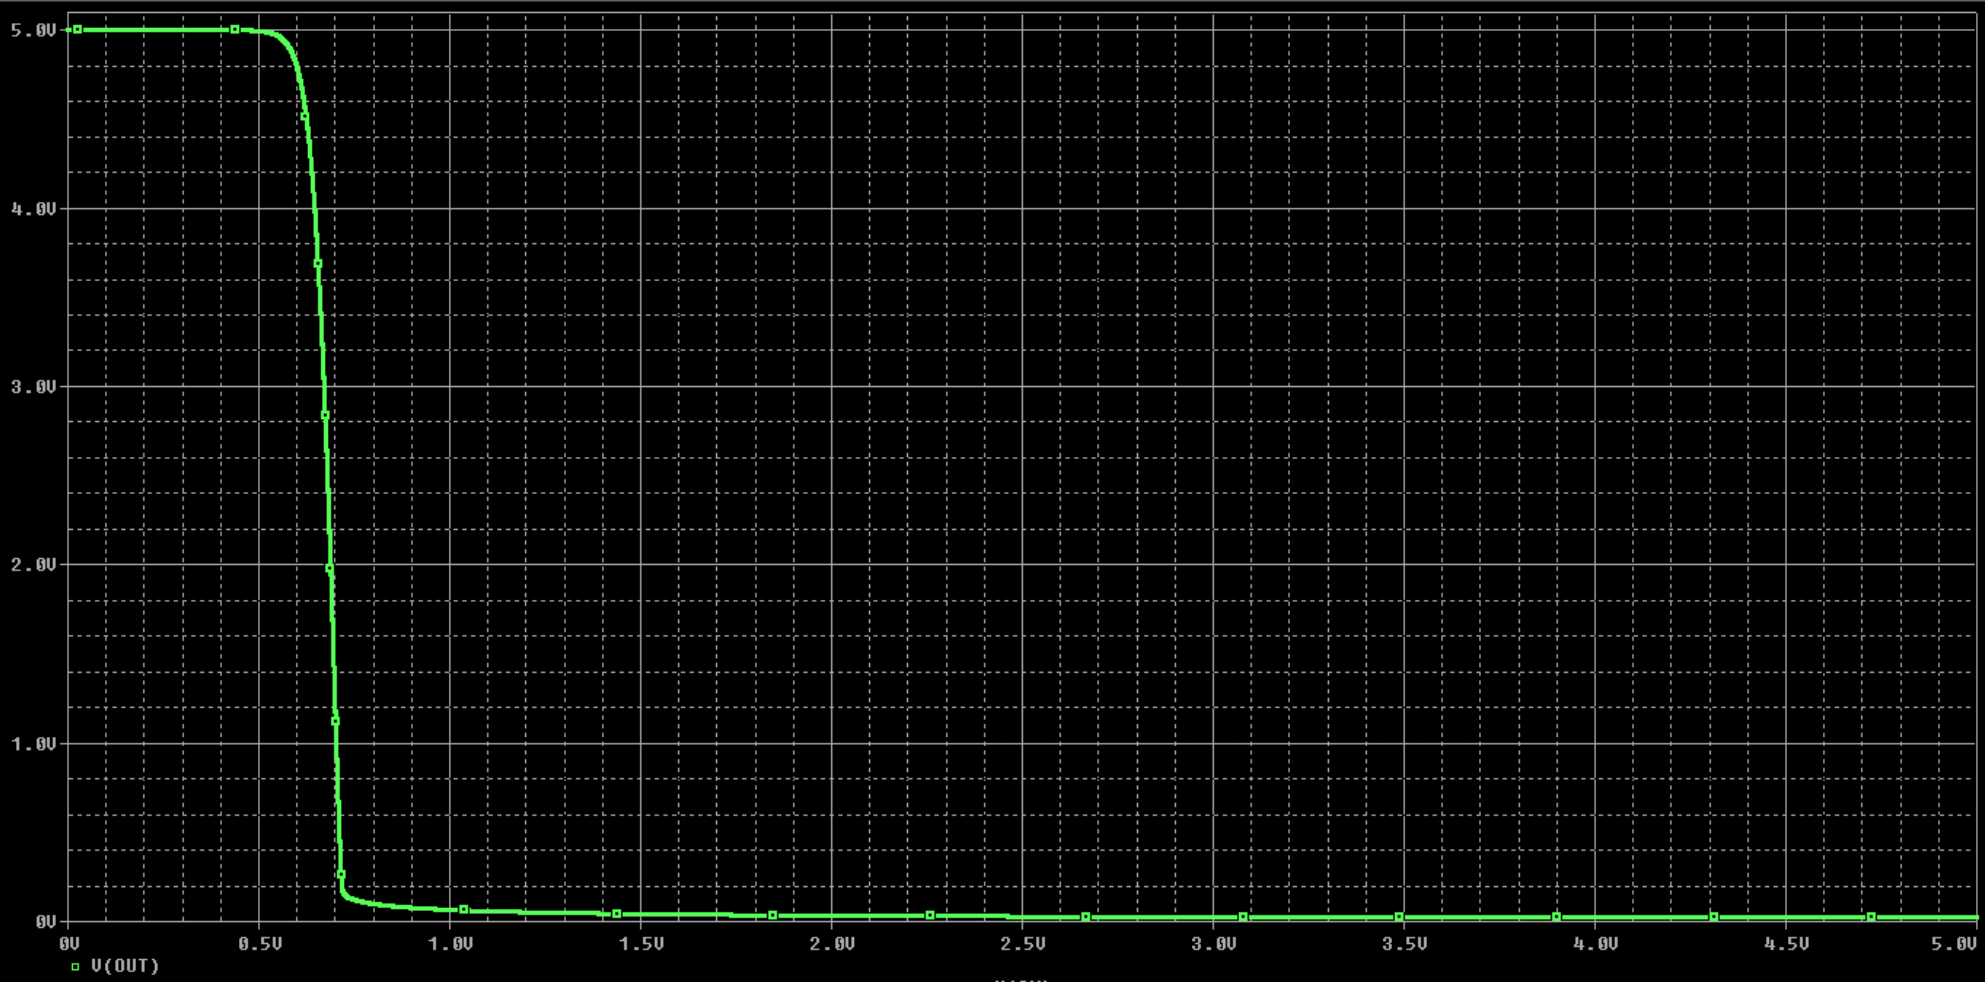
\includegraphics[scale=0.35,angle=0]{rtl_not_transfer.png}
    \caption{Tensione di uscita della porta NOT}
    \label{not_transfer}
\end{figure}
\\Al contrario, durante la fase di transizione, corrispondente all'omonima regione, il transistor non è in saturazione (quindi la tensione di collettore non è pari a $0,2 - 0,3\,V$) ma si trova in regione \textit{attiva diretta} questo perché si sa che la corrente in base scorre positiva quindi, andando per esclusione, ci si trova proprio in quella regione.
\begin{figure}[h]
    \centering
    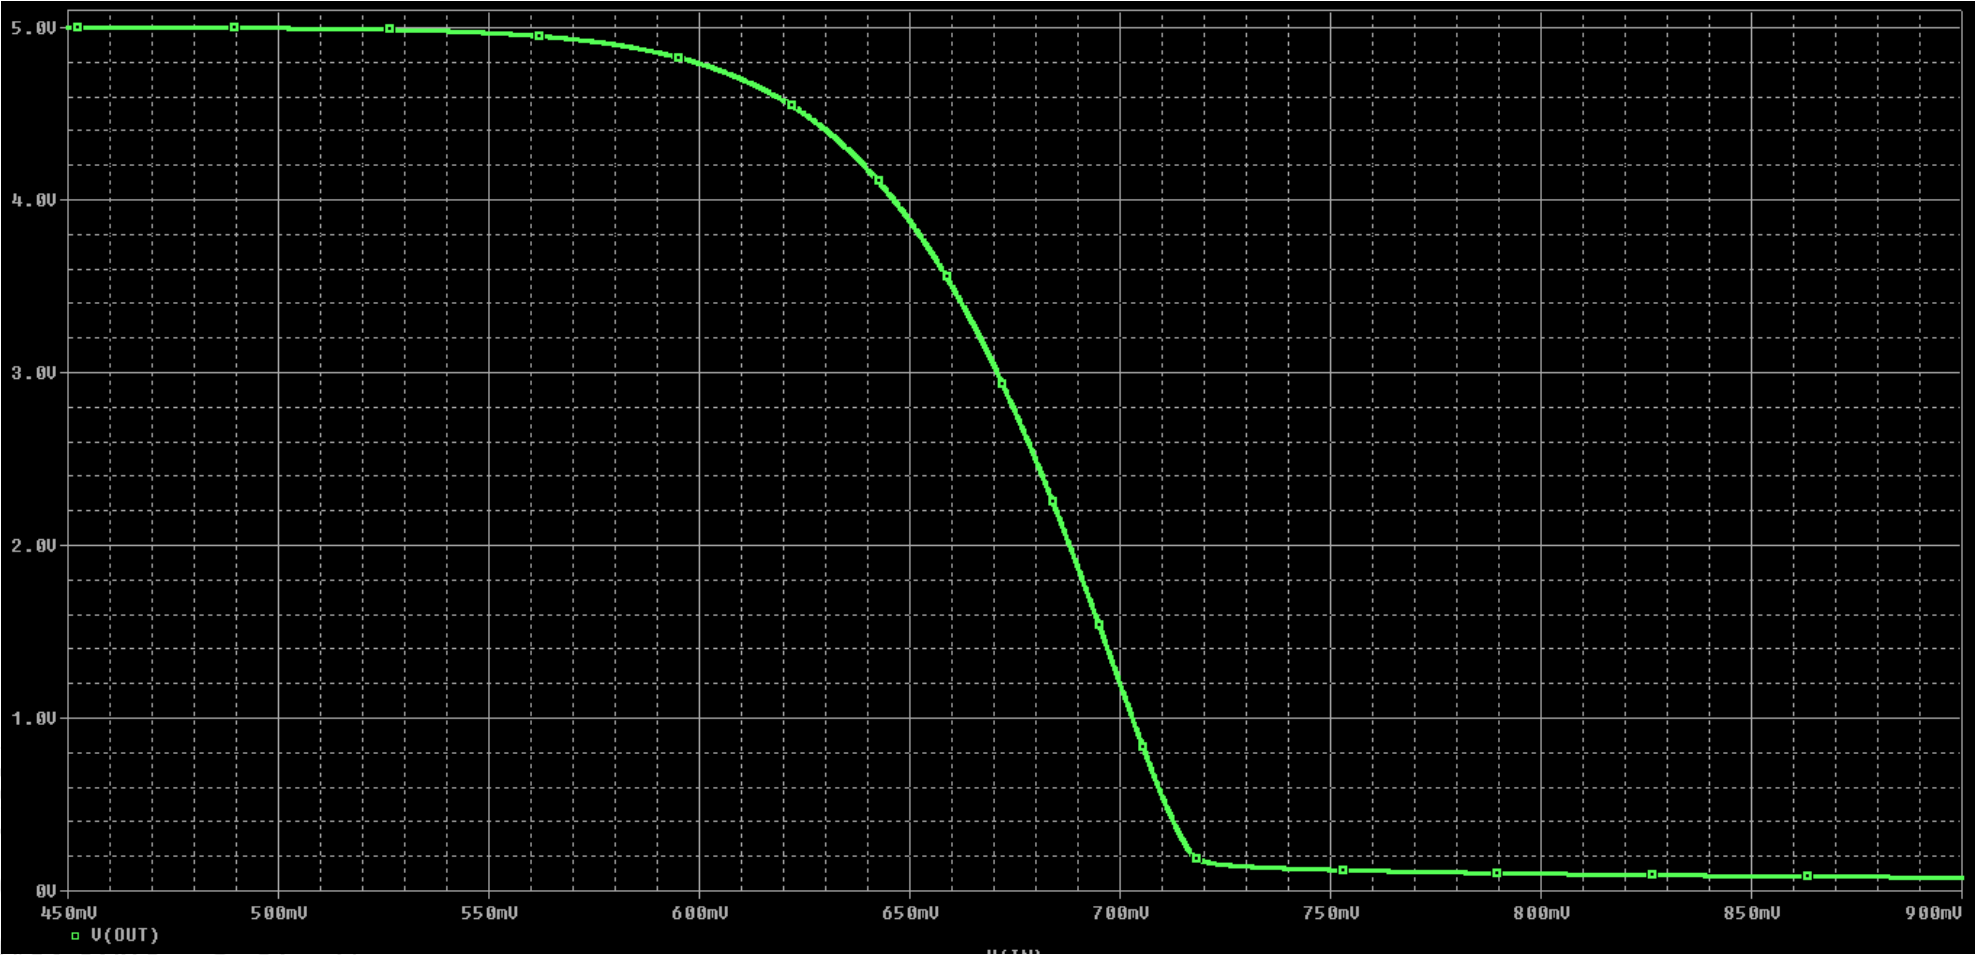
\includegraphics[scale=0.35,angle=0]{rtl_not_transfer_zoom.png}
    \caption{Zoom sulla regione di transizione della porta NOT}
    \label{not_transfer_zoom}
\end{figure}
\\Quando la tensione in ingresso raggiunge i $700 - 750\,mV$, la tensione di collettore raggiunge gli $0,2\,V$. La curva rappresentata non è altro che l'esponenziale rovesciato della corrente di base che tende ad essere esponenziale in quanto la base del transistor è un diodo (quindi riprende il grafico in figura \ref{i_diodo}), e se la corrente di base è esponenziale anche quella di collettore, moltiplicata per il guadagno $h_{fe}$, vorrebbe essere esponenziale. Tuttavia quando la tensione di collettore raggiunge $0,2\,V$ non può scorrere ulteriore corrente dunque il transistor in saturazione e l'uscita diventa bassa.

\subsection{Parametri statici}
A partire da tutte queste considerazioni è già possibile stimare alcuni parametri statici della famiglia logica:
\begin{itemize}
    \item Poiché $V_{iH}$ è la tensione di ingresso minima oltre la quale l'uscita è sicuramente bassa, si ha:
    \begin{equation}
        V_{iH} = 0,75\,V
        \label{v_ih_not}
    \end{equation}
    \item Essendo $V_{iL}$ la tensione di ingresso al di sotto della quale l'uscita è sicuramente alta, si pone:
    \begin{equation}
        V_{iL} = 0,6\,V
    \end{equation}
    \item Per un ingresso alto, quindi con una tensione di ingresso pari a $V_{iH} = 0,75\,V$, sapendo che la tensione di base vale $R_{b} = 450\,\Omega$ e supponendo che sulla base ci sia una tensione di circa $0,6 - 0,65\,V$ si ottiene:
    \begin{equation}
        I_{iH} = \frac{0,75\,V - 0,65\,V}{450\,\Omega} \approx 200\,\mu A
        \label{i_ih_not}
    \end{equation}
    se invece la tensione di ingresso sale, prendendo per esempio una tensione di ingresso di $5\,V$, si ha
    \begin{equation*}
        I_{iH} = \frac{5\,V - 0,7\,V}{450\,\Omega} \approx 9.5\,mA
    \end{equation*}
    \item Se l'ingresso è basso, quindi collegato a $0\,V$, esso vede la resistenza di base e la giunzione tra la base e l'emettitore anch'esso collegato a massa $0\,V$ dunque non scorre corrente:
    \begin{equation}
        I_{iL} \approx 0\,A
        \label{i_il_not}
    \end{equation}
    l'unica corrente che potrebbe scorrere è una leggera corrente di perdita inversa $I_{0}$ che va verso terra ed è dovuta al carico del collettore ma è comunque trascurabile
    \item A tensione in uscita alta, poiché tra collettore ed emettitore non scorre corrente e sulla resistenza di collettore $R_c$ non cade tensione, si ha:
    \begin{equation}
        V_{oH} = 5\,V
        \label{v_oh_not}
    \end{equation}
    ma per far ciò non è stato collegato niente all'uscita. Se si collegasse all'uscita un altro ingresso RTL analogo (resistenza di base e giunzione base-emettitore entrambe a $0\,V$) si avrebbe una resistenza collegata con una giunzione pn, dunque scorrerebbe corrente e sull'uscita non ci sarebbero più $5\,V$ ma molti meno
    \item Se infine la tensione in uscita è bassa, il transistor è in saturazione ed ha una tensione $V_{ce}$ che può essere al massimo $0,2\,V$, dunque:
    \begin{equation}
        V_{oL} = 0,2\,V
        \label{v_ol_not}
    \end{equation}
    questo è vero per \textit{qualsiasi} corrente di collettore, ovvero tutte le correnti di collettore che non fanno uscire il transistor dalla saturazione. Tuttavia se l'uscita è bassa e guida altri ingressi, essa andrà a prelevare una certa $I_{iL}$ dagli altri ingressi ma essa, come detto nella \eqref{i_il_not}, è nulla quindi a livello logico basso si è abbastanza sicuri che non succede niente di particolare in quanto non scorre corrente in ingresso e il transistor può essere considerato in saturazione
\end{itemize}
Da tutti questi parametrici statici è ora possibile ricavare ulteriori grandezze d'interesse:
\begin{itemize}
    \item Note le tensioni in ingresso e in uscita per i due livelli logici possibili è possibile calcolare il margine di rumore alto e basso:
    \begin{equation*}
        \textit{NM}_{H} = V_{oH} - V_{iH} = 5\,V - 0,75\,V = 4,25\,V
    \end{equation*}
    abbastanza alto
    \begin{equation*}
        \textit{NM}_{L} = V_{iL} - V_{oL} = 0,6\,V - 0,2\,V = 0,4\,V
    \end{equation*}
    relativamente basso. Da qui si ricava infine il rumore elettrico:
    \begin{equation}
        \textit{NM} = min(\textit{NM}_{L},\, \textit{NM}_{H}) = 0,4\,V
    \end{equation}
    si nota che questa porta logica è \textit{molto asimmetrica} e il suo margine di rumore è tutto mangiato dalla parte bassa. Questo significa che per un ingresso basso di $0,2\,V$ la porta logica lo considera basso fino a $0,6\,V$ ma se c'è un rumore di $0,4\,V$, quindi lo fa salire a $0,6\,V$, non è più garantito che l'ingresso sia considerato correttamente
    \item Avendo visto che il NOT non pone problemi quando il suo ingresso è basso, perché non ha requisiti in corrente (vedi \eqref{i_il_not}) e l'uscita è in saturazione quindi in una situazione buona per comandare un carico, il fattore critico della porta è l'uscita alta. Infatti con l'ingresso basso e l'uscita alta che va a pilotare altri ingressi (cioè un certo numero di giunzioni pn e resistenze verso masso), il transistor è in interdizione quindi il circuito è composto da una tensione di $5\,V$ più una resistenza da $640\,\Omega$ (come si vede in figura 5.1) e le \textit{n} coppie resistenza-diodo. Per determinare \textit{n}, cioè il fan-out, si deve considerare la tensione applicata nel nodo alla destra della resistenza da $640\,\Omega$ che precede le \textit{n} coppie. Volendo che il segnale (corrispondente all'uscita della porta) sia alto si sa che devono esserci almeno $0,75\,V$ secondo la \eqref{v_ih_not}, dunque ai capi della resistenza da $640\,\Omega$ si deve avere
    \begin{equation*}
        V_{R_{c}} < 5\,V - 0,75\,V
    \end{equation*}
    ma $V_{R_{c}} = I \cdot R_{c}$, dunque
    \begin{equation*}
        I \cdot R_{c} \leq 5\,V - 0,75\,V \Rightarrow I \leq \frac{5\,V - 0,75\,V}{640\,\Omega} = 6,6\,mA
    \end{equation*}
    che è la corrente massima che può scorrere nella resistenza $R_c$ prima che il nodo, rappresentante l'uscita della porta, vada sotto la $V_{iH} = 0,75\,V$ delle altre porte logiche. Questa corrente si può cedere alle \textit{n} porte logiche collegate. Si sa ora, grazie alla \eqref{i_ih_not}, che nel caso di ingresso alto ogni porta logica consuma una corrente pari a $I_{iH} \approx 200\,\mu A$, per cui:
    \begin{equation}
        \textit{Fan-out} = \frac{6,6\,mA}{200\,\mu A} = 33
    \end{equation}
    \item Quando l'uscita è bassa il transistor è in saturazione e, secondo la \eqref{v_ol_not}, ai capi di $R_c$ è applicata una tensione di $5\,V - 0,2\,V = 4,8\,V$ quindi la corrente che scorre attraverso $R_c$ è data da $I_{R_{c}} = \frac{4,8\,V}{640\,\Omega} = 7,5\,mA$. È l'unica corrente che scorre, non si deve considerare quella che scorre nella base del transistor perché questa corrente non fa parte della porta logica. Dunque si ottiene:
    \begin{equation*}
        P_{L} = 5\,V \cdot 7,5\,mA = 37,5\,mW
    \end{equation*}
    Quando invece l'uscita è alta la corrente che scorre in $R_c$ è nulla e la corrente in ingresso, secondo la \eqref{i_il_not}, è nulla dunque la cella è di fatto spenta:
    \begin{equation*}
        P_{H} = 0\,mW
    \end{equation*}
    Si arriva infine a definire la potenza media:
    \begin{equation}
        P = \frac{P_{L} + P_{H}}{2} = \frac{37,5\,mW + 0\,mW}{2} = 18\,mW
    \end{equation}
    quindi una singola cella logica che compone la porta NOT in logica RTL consuma $18\,mW$ di potenza
\end{itemize}

\subsection{Parametri dinamici}
Per quanto riguarda i parametrici dinamici si può dire che è un circuito abbastanza veloce grazie alla sua semplicità. Quando si deve accendere il dispositivo si incontra inizialmente la resistenza di base da $450\,\Omega$ (decisamente bassa, è questo il motivo per cui ha un consumo molto elevato) che pompa corrente nella base. Tutta questa corrente viene amplificata dal transistor che permette di abbassare (assorbendo corrente) la resistenza di carico $R_c$ e le eventuali \textit{capacità parassite} che potrebbero essere presenti. Avendo molta corrente sia in base che nel collettore saranno sufficienti pochi nanosecondi (circa $5\,nS$) per accendere il transistor.

Analogamente l'operazione di spegnimento del dispositivo, ovvero l'azione di rilasciare l'uscita per farla ritornare alta, è anch'essa molto veloce e richiede solo pochi nanosecondi (sempre circa $5\,nS$). Quando il transistor è acceso si sta facendo scorrere corrente nella base che, per costruzione, è una giunzione pn che si carica con i portatori minoritari. Quando si vuole spegnere la base si devono svuotare i portatori minoritari accumulati, cioè si deve far scorrere una corrente inversa per eliminare la carica accumulata nella base. Tutta questa operazione può essere effettuata rapidamente perché per svuotare le cariche si incontra la resistenza di base e il transistor della porta precedente che è in saturazione e può quindi tirare molta corrente. Per quanto detto, i tempi di propagazione $t_{p_{HL}}$ e $t_{p_{LH}}$ sono entrambi molto piccoli, dell'ordine dei nanosecondi:
\begin{equation}
    t_{p_{HL}} \approx 5\,nS \text{ \, \, } t_{p_{LH}} \approx 5\,nS
\end{equation}
Ricordando che la potenza dissipata è $18\,mW$, si può calcolare il prodotto ritardo-potenza (più piccolo è e meglio è perché significa che si ha poco ritardo e/o poco consumo):
\begin{equation}
    \textit{DP} = t_{p} \cdot P = 5\,nS \cdot 18\,mW = 90\,pJ
\end{equation}
Si può dire che il dispositivo ha un comportamento dinamico \textit{simmetrico}, cioè i due tempi di propagazione sono simili tra loro.

Se si raddoppiassero tutte le resistenze si dimezzerebbero le correnti e questo comporta un dimezzamento della potenza. Ma l'accensione del dispositivo dipende da quanta corrente passa nella resistenza di base e nella giunzione pn tra base ed emettitore dunque raddoppiando $R_b$ la corrente si dimezza e si dimezza anche la corrente che scorre tra collettore ed emettitore e questo implica che il tempo di propagazione raddoppia. Anche per eliminare i portatori minoritari sarà richiesto il doppio del tempo. Dunque entrambi $t_{p_{HL}}$ e $t_{p_{LH}}$ raddoppiano, la potenza \textit{P} si dimezza e quindi \textit{DP} rimane \textit{invariato} e dipende solo da \textit{come} è costruita la porta logica.

\chapter{TTL}
È la più recente evoluzione della famiglia logica RTL. \textbf{TTL} sta per \textbf{Transistor Transistor Logic}, così chiamata perché prevede l'impiego di due transistor.

\section{NOT base}
La porta \textbf{NOT} nella sua versione \textit{base} è composta da due resistenze, una delle quali è la resistenza di carico, e due transistors. La versione in logica TTL è data dal seguente circuito:
\begin{figure}[h]
    \centering
    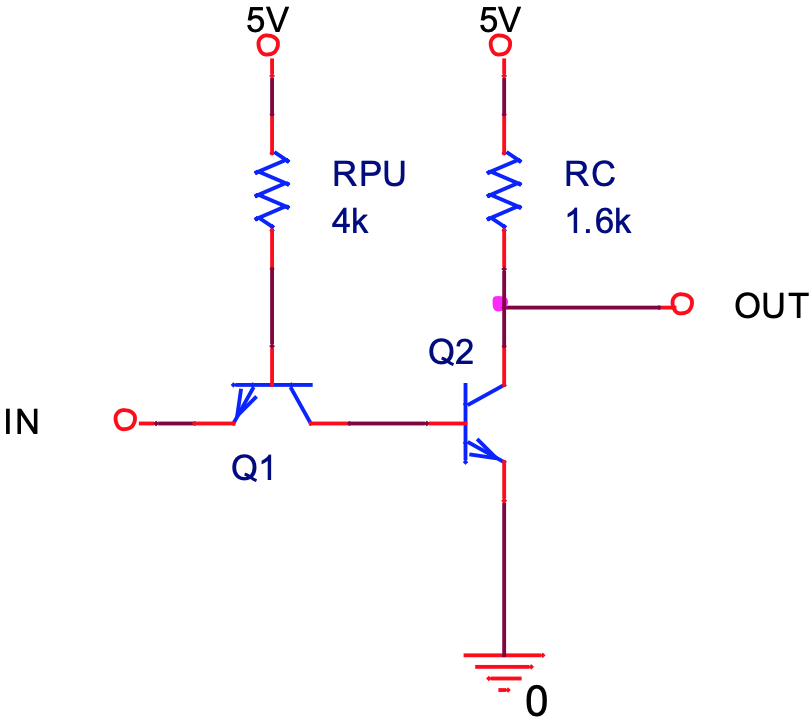
\includegraphics[scale=0.4,angle=0]{ttl_not_base.png}
    \caption{Struttura base del NOT in logica TTL}
    \label{not_base}
\end{figure}
\\Quando l'ingresso \textit{IN} della porta è \textit{basso} (si considera una tensione di $0\,V$) la giunzione tra la base e l'emettitore del transistor $Q_1$ è polarizzata \textit{direttamente}, dunque scorre una corrente dalla base all'emettitore passate anche nella resistenza $R_{pu}$. Se tra la base e l'emettitore è presente una tensione di $0,7\,V$ e sull'emettitore è applicata la tensione di ingresso di $0,2\,V$ (difficilmente è effettivamente nulla), ai due capi della resistenza $R_{pu}$ sono applicati due potenziali da $5\,V$ e $0,9\,V$ e la corrente che scorre nella resistenza, cioè la corrente in base del transistor, vale:
\begin{equation}
    I_{R_{pu}} = \frac{V_{R_{pu}}}{{R_{pu}}} = \frac{5\,V - 0,9\,V}{4\,k\Omega} \approx 1\,mA
    \label{i_rpu}
\end{equation}
Data questa corrente in base, $Q_1$ non può che trovarsi o in saturazione o in regione attiva diretta. Per essere in regione attiva diretta dovrebbe scorrere tanta corrente nel suo collettore ma questa corrente proverrebbe dalla base del transistor $Q_2$ che ha una giunzione pn tra la base e l'emettitore, questo comporta che non può scorrere una corrente che sia uscente dalla base di $Q_2$ e quindi $I_{c_1} \approx 0\,A$ e $Q_1$ si trova sicuramente in \textit{saturazione}. Ricevendo $0,2\,V$ in ingresso e trovandosi in saturazione, $Q_1$ ha una tensione tra collettore ed emettitore pari a $V_{ce-sat} = 0,2\,V$ e sul collettore è presente un potenziale di $0,4\,V$. Con $0,4\,V$ massimi sul collettore, la base di $Q_2$ (in particolare la giunzione tra base ed emettitore) \textit{non} si può accendere, ma allora se $Q_2$ è spento significa che l'uscita \textit{OUT} dell'intero circuito è \textit{alta} perché \textit{non} scorre corrente attraverso il carico $R_c$.

Se invece \textit{IN} è \textit{alto} la tensione tra la base e l'emettitore di $Q_2$ è compresa tra $0\,V$ e $0,75\,V$ e, poiché tra la base e il collettore di $Q_1$ è presente una giunzione pn, sulla base di $Q_1$ c'è una tensione compresa tra $0\,V$ e $1,4 - 1,5\,V$ (non oltre perché si avrebbero le giunzioni base-collettore di $Q_1$ e base-emettitore di $Q_2$ entrambe pienamente polarizzate direttamente). Dunque se \textit{IN} è alto a $5\,V$, la giunzione tra la base e l'emettitore di $Q_1$ rimane polarizzata \textit{inversamente} mentre la giunzione tra la base e il collettore di $Q_1$ viene tirata su dalla \textbf{resistenza di pull-up} $R_{pu}$ e si polarizza \textit{direttamente}: questo comporta che $Q_1$ si trova in regione \textit{attiva inversa}. In regione attiva inversa il guadagno in corrente di $Q_1$ è $h_{fe} \approx 0$, quindi la corrente che scorre dall'ingresso è molto poca. In questa situazione scorre corrente nella giunzione tra base e collettore di $Q_1$ e nella giunzione tra base ed emettitore di $Q_2$, dunque $Q_2$ è acceso, va in saturazione e \textit{OUT} è \textit{bassa}.

I principali pregi del NOT in TTL rispetto a quello in RTL sono i seguenti:
\begin{itemize}
    \item Quando in fase dinamica, con ingresso inizialmente alto, si vuole spegnere il dispositivo abbassando l'ingresso e facendo diventare l'uscita alta, in $Q_1$ la giunzione tra la base e l'emettitore si polarizza direttamente e il transistor passa in regione attiva diretta assorbendo le cariche minoritarie dalla base del transistor $Q_2$ mediante il suo guadagno $h_{fe}$, quindi lo spegnimento è molto veloce come lo è altrettanto la transizione $L \rightarrow H$ in uscita (già sapevamo che la transizione in uscita $H \rightarrow L$ è veloce perché accendere un transistor è sempre più facile che spegnerlo)
    \item La corrente assorbita sull'ingresso è limitata e in particolare, mentre nel caso RTL quando l'ingresso era alto si doveva fornire un corrente che poteva eventualmente diventare notevole, in questo caso se l'ingresso è alto non scorre corrente nell'ingresso quindi il caso di ingresso alto è un caso favorevole. Quando invece l'ingresso è basso si ha un valore fisso di corrente che dipende da $R_{pu}$
    \item Lo stadio di uscita è composto dalla resistenza $R_c$ come nel caso RTL, quindi quando l'uscita è bassa non ci sono problemi (transistor che va in saturazione) mentre se l'uscita è alta c'è la resistenza $R_c = 1,6\,k\Omega$ maggiore di quella in RTL per poter diminuire la potenza consumata dalla porta logica pur avendo minor capacità di guidare l'uscita ma questo è ragionevole perché serve a guidare la $I_{iH}$ delle altre porte logiche che si è detto essere molto piccola
\end{itemize}
In generale, quando l'uscita va bassa il transistor tira la corrente verso il basso ma quando l'uscita va alta si ha una modesta resistenza $R_c$ che alza la corrente.

\section{Enhanced NOT}
A causa della sua scarsa efficienza, la versione base del NOT in logica TTL è stata rapidamente rimpiazzata con un suo miglioramento chiamato \textbf{enhanced NOT}. Il circuito è più complesso: è aumentato il numero di transistors e delle resistenze ed è stato introdotto un diodo. Nello specifico, tra il transistor $Q_1$ (con la relativa resistenza di pull-up $R_{pu}$) e il transistor $Q_2$ è stato inserito uno stadio intermedio composto da due resistenze $R_{pu_1}$ e $R_{pd}$ e il transistor $Q_3$ (tutti e tre servono per guidare i transistor $Q_2$ e $Q_4$ con due segnali in opposizione di fase), inoltre la resistenza di carico $R_c$ da $1,6\,k\Omega$ è stata sostituita con un nuovo carico composto dal diodo $D_1$, il transistor $Q_4$ e la resistenza di carico $R_c$ da $130\,\Omega$. Il transistor $Q_4$ in uscita aiuta a migliorare le performance. 
\begin{figure}[h]
    \centering
    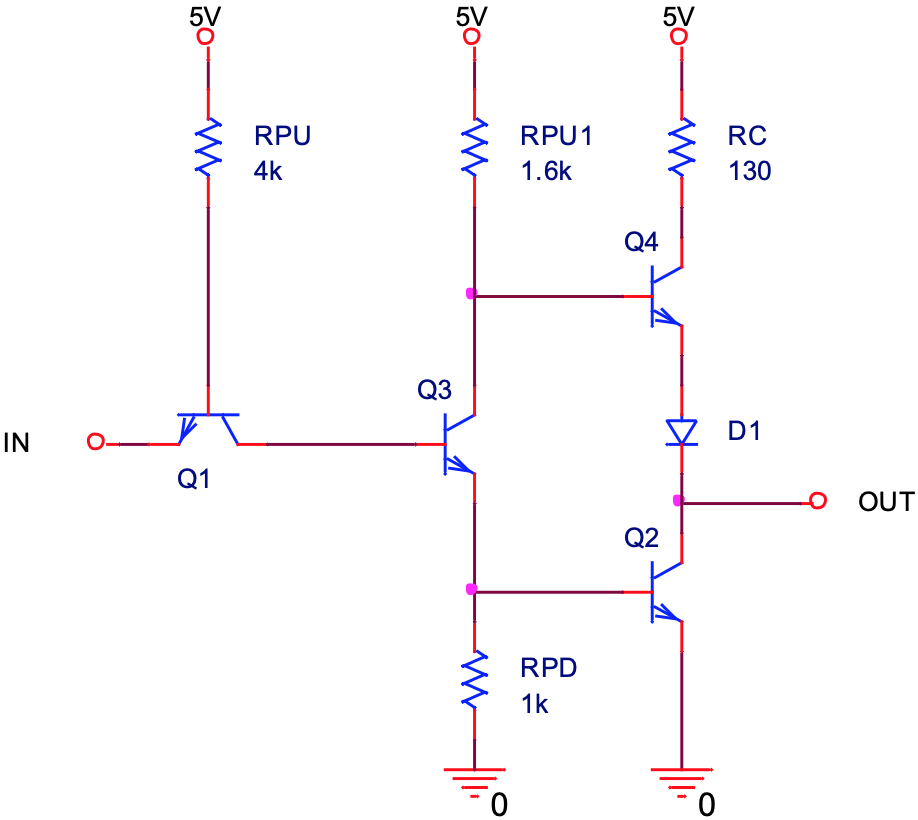
\includegraphics[scale=0.4,angle=0]{ttl_not_enh.png}
    \caption{Struttura dell'enhanced NOT}
    \label{not_enh}
\end{figure}
\\Quando $Q_3$ è \textit{spento}, in $R_{pu_1}$ e $R_{pd}$ non scorre corrente, quindi l'ingresso nella base di $Q_4$ è alto mentre quello nella base di $Q_2$ è basso. Questo comporta che $Q_2$ è spento e $Q_4$ può essere acceso se scorre corrente dalla sua base all'emettitore, passante poi in $D_1$.

Viceversa, se scorre corrente attraverso $Q_3$ (quindi $Q_3$ è accesso la corrente scorre anche attraverso $R_{pu_1}$ e $R_{pd}$) c'è una caduta di tensione su $R_{pu_1}$ e su $R_{pd}$, quindi l'ingresso nella base di $Q_4$ è basso e quello nella base di $Q_2$ è alto. In queste condizioni, $Q_4$ è spento mentre $Q_2$ è acceso.

L'obiettivo del miglioramento era quello di aggiungere qualcosa nello stadio di uscita ma questa aggiunta ha implicato l'inserimento dello stadio intermedio appena descritto. In seguito a queste modifiche:
\begin{itemize}
    \item Lo stadio di uscita è stato effettivamente migliorato perché il transistor $Q_4$ aggiunto è in grado di fornire una piccola corrente all'uscita che può quindi essere tirata verso l'alto più velocemente
    \item Al contrario, il transistor $Q_2$ è nuovamente difficile da spegnere perché il suo spegnimento può essere effettuato solo tramite la \textbf{resistenza di pull-down} $R_{pd}$ posta a $1\,k\Omega$ per esigenze di consumo
\end{itemize}
Il guadagnato in velocità ottenuto inserendo $Q_4$ nello stadio di uscita è stato pagato in termini di velocità di commutazione quando si deve spegnere $Q_2$, ovvero quando si deve fare il passaggio $L \rightarrow H$ in uscita.

\subsection{Caratteristica di enhanced NOT}
La \textbf{caratteristica ingresso-uscita} dell'enhanced NOT ha un andamento che può essere schematizzato in tre fasi. Per valori bassi di tensione l'uscita rimane alta, segue una fase in cui l'uscita decresce lentamente e infine si ha una terza fase in cui l'uscita crolla fino a stabilizzarsi su valore di tensione basso. Analizzando più nel dettaglio tramite la figura \ref{enh_zoom} si nota che nella seconda fase la tensione di uscita decresce \textit{linearmente}. Per una tensione in ingresso compresa tra $0\,V$ e circa $1,5\,V$ (corrispondente all'intervallo di tensioni in cui l'uscita inizialmente rimane costante e poi decresce) si nota che in corrispondenza di $0,5 - 0,6\,V$ inizia la fase di decrescita lineare.
\begin{figure}[h]
    \centering
    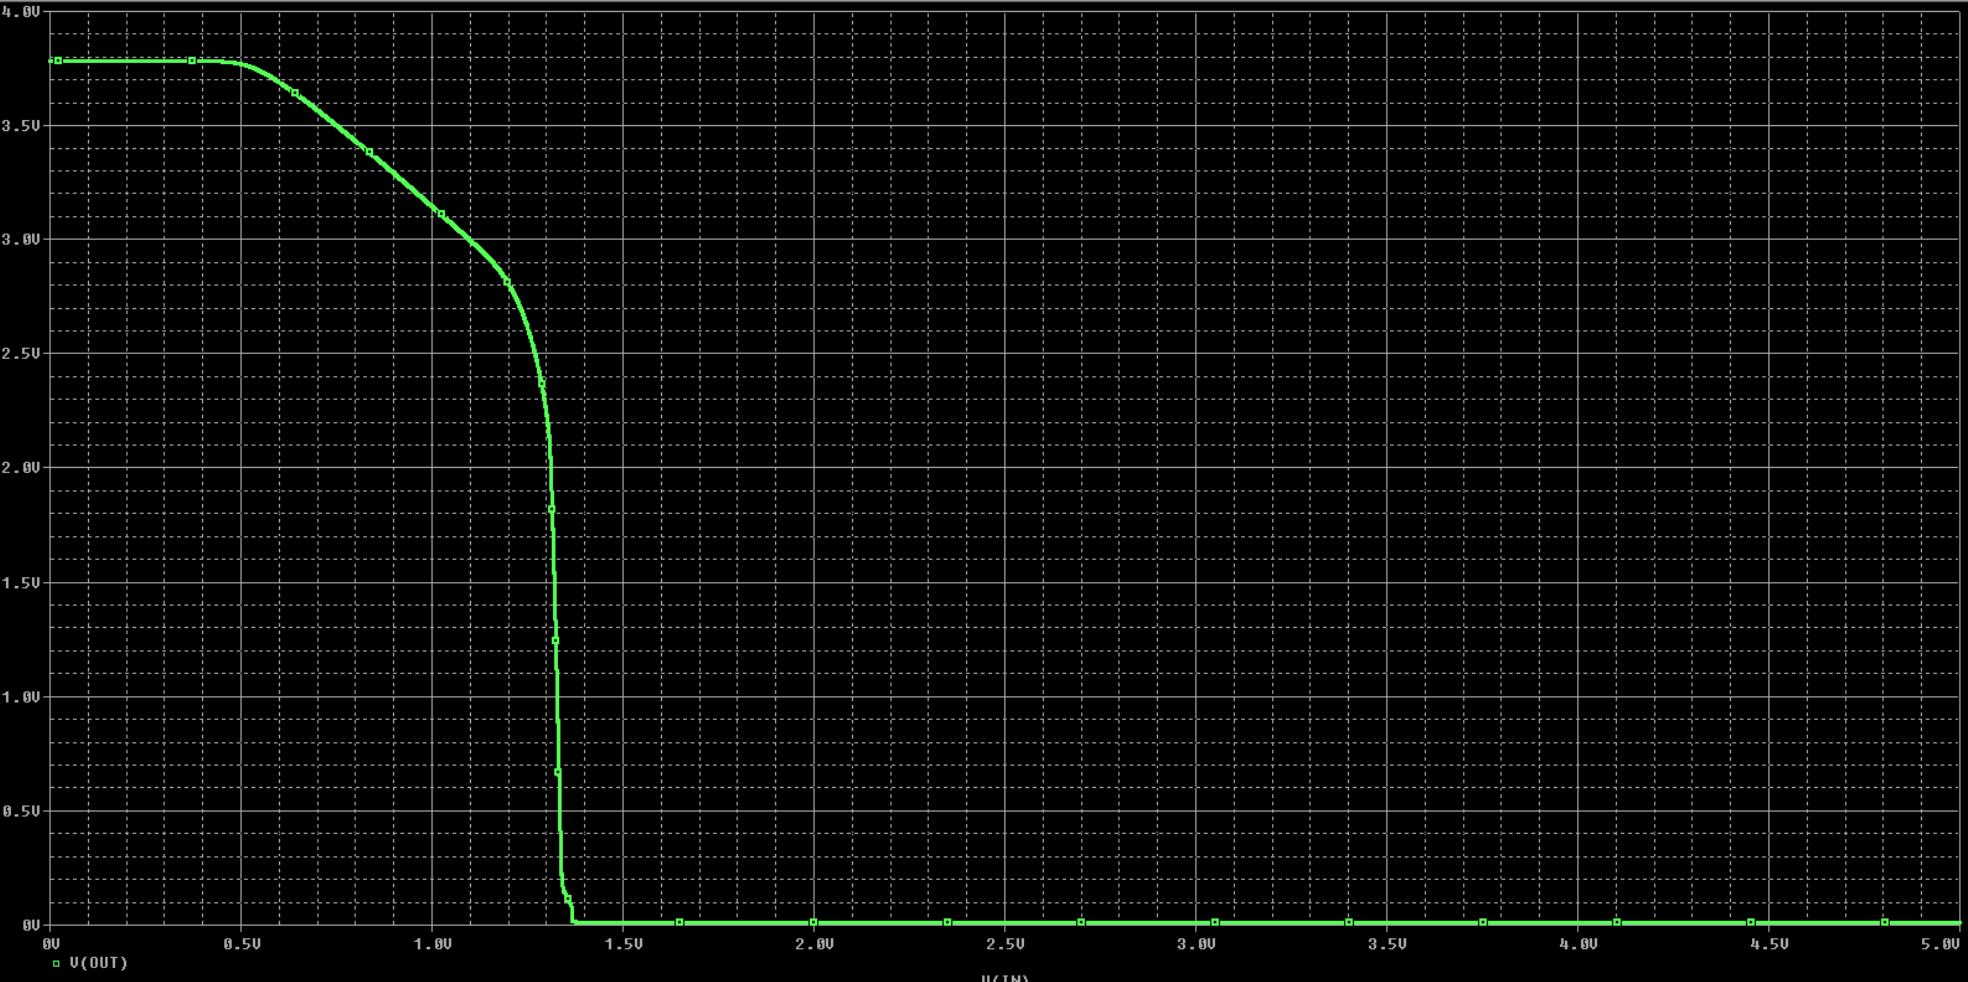
\includegraphics[scale=0.35,angle=0]{ttl_not_enh_transfer.png}
    \caption{Tensione in uscita dall'enhanced NOT}
\end{figure}

Analizzando la struttura circuitale dell'enhanced NOT riportata in figura \ref{not_enh} si nota che per un ingresso basso (tensione in ingresso di $0\,V$), sull'emettitore di $Q_1$ è presente un potenziale positivo di $0,7\,V$ e sul collettore, poiché c'è una normale giunzione pn, può esserci un potenziale negativo che vale al massimo $0,7\,V$. Dunque quando l'ingresso è basso, la base di $Q_1$ è tenuta alta dal pull-up $R_{pu}$ e il collettore sta a circa $0\,V$. Ci si trova dunque nella prima fase in cui l'uscita rimane alta.
\begin{figure}[h]
    \centering
    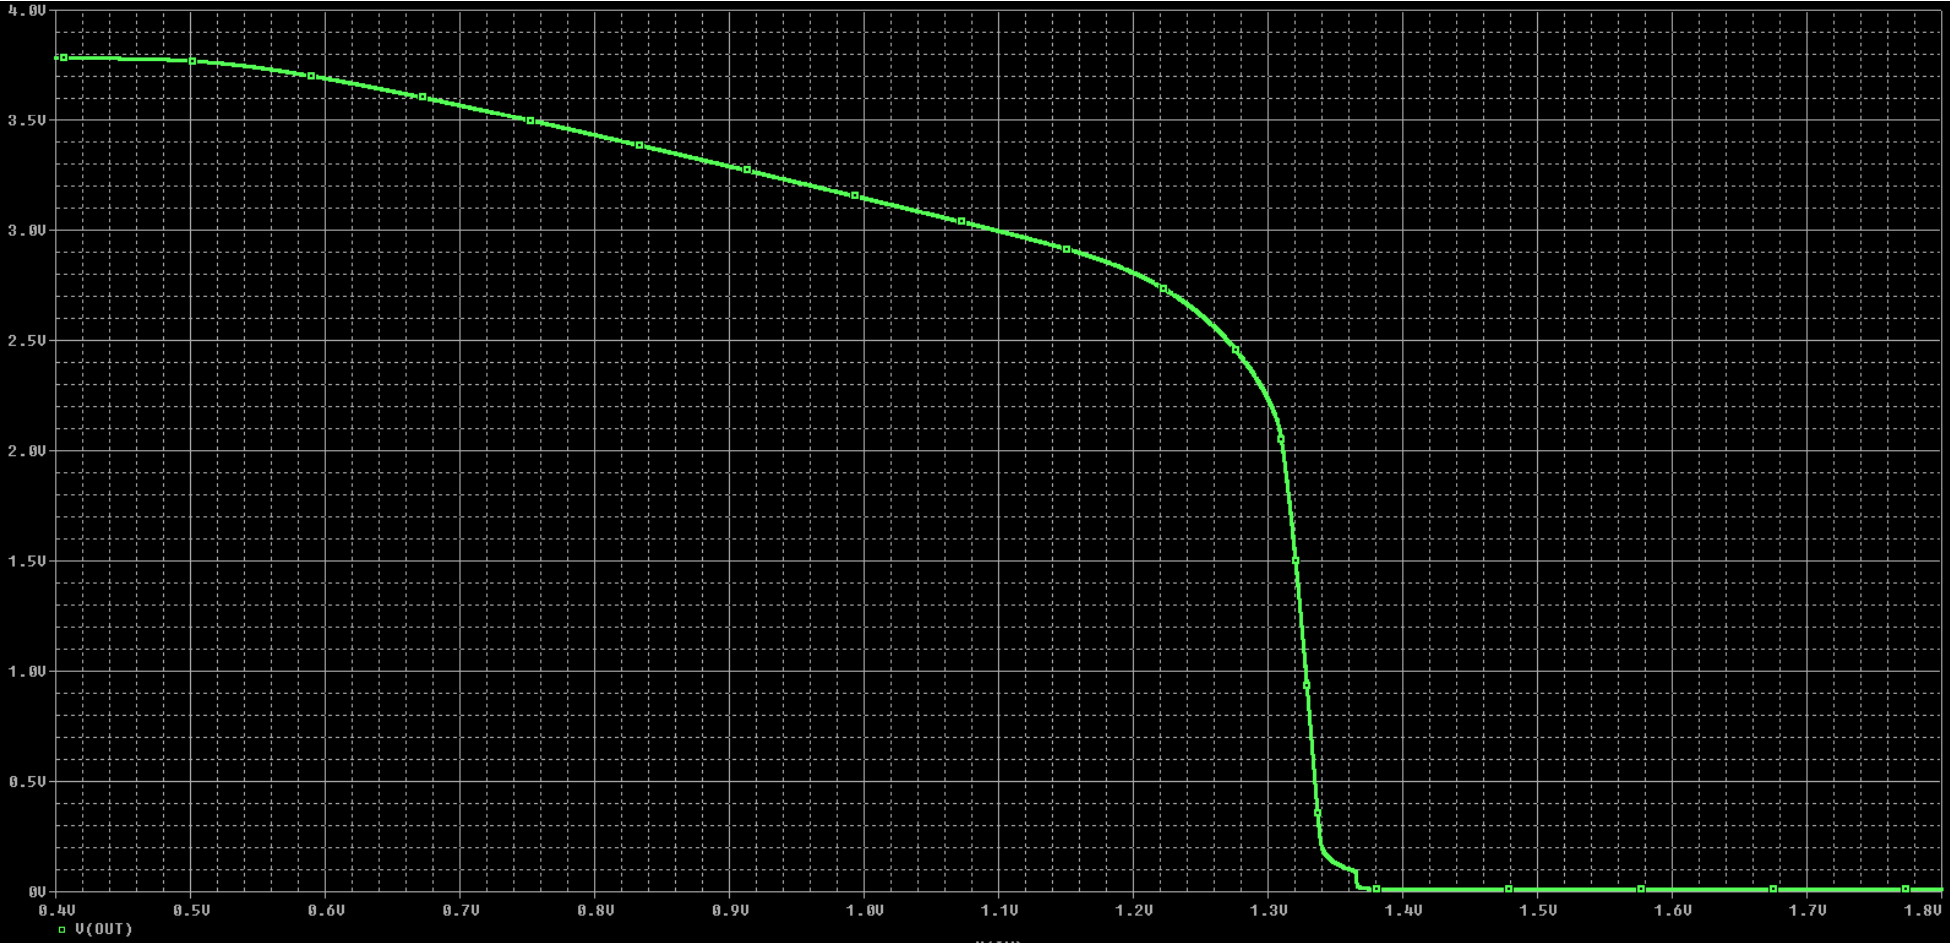
\includegraphics[scale=0.35,angle=0]{ttl_not_enh_transfer_zoom.png}
    \caption{Zoom sulla regione di transizione}
    \label{enh_zoom}
\end{figure}

Se ora si aumenta la tensione dell'emettitore (quindi \textit{IN}) a circa $0,5\,V$, tra emettitore e base di $Q_1$ si passa da una tensione di $0,7\,V$ ad una tensione di $0,7\,V + 0,5\,V = 1,2\,V$ e poiché sulla giunzione base-collettore di $Q_1$ si può avere al massimo $0,7\,V$, tra la base e l'emettitore di $Q_3$ si crea una tensione di $0,5\,V$ (come in ingresso) e quella giunzione inizia a polarizzarsi. Se il transistor $Q_3$ inizia ad accendersi comincia a scorre corrente dal collettore all'emettitore di $Q_3$, cioè da $R_{pu_1}$ a $R_{pd}$. Ma se scorre corrente nello stadio intermedio, la caduta di tensione ai capi di $R_{pu_1}$ è \textit{direttamente proporzionale} alla corrente che ci scorre. Per poter calcolare questa corrente si considera che tra la base e l'emettitore di $Q_3$ c'è una tensione di $0,5\,V$ e ciò che rimane cade sulla resistenza $R_{pd}$. Il fatto che il nodo tra $R_{pu_1}$ e il collettore di $Q_3$ scenda di tensione fa sì che anche l'uscita (l'emettitore) del transistor $Q_4$ vada verso il basso, quindi l'uscita scende linearmente (perché, come detto, la tensione di base di $Q_4$ scende). Ci si trova dunque nella seconda fase di decrescita lineare con pendenza della retta intorno a $-\frac{1}{2}$.

A partire da $1,2\,V$ in ingresso, cioè da quando la tensione sull'emettitore di $Q_3$ è salita di circa $0,7\,V$, si accende il transistor $Q_2$ che tira bruscamente verso il basso l'uscita del circuito. Ci si trova dunque nella terza fase. Se si continua ad aumentare la tensione in ingresso la corrente passa attraverso $R_{pu}$, tramite la giunzione base-collettore di $Q_1$ va nella base di $Q_3$, da lì tramite l'emettitore va in $Q_2$ e infine esce dall'emettitore di $Q_2$ andando a terra. Non viene fornita nessuna corrente all'ingresso.

La corrente di carico $R_c$ e il diodo $D_1$ sono stati inseriti per ottimizzare la forma d'onda di uscita. In particolare $R_c$ serve perché in fase di commutazione dinamica del livello logico (in entrambi i sensi) esiste un piccolo istante di tempo in cui $Q_4$ e $Q_2$ sono accesi contemporaneamente (perché è più difficile spegnere un transistor acceso piuttosto che accenderne uno spento: il transistor spento si accende velocemente mentre quello acceso si spegne lentamente) e in quell'istante la corrente scorre in entrambi da $Q_4$ a $Q_2$. Per limitare questa corrente si inserisce la resistenza $R_c$ che limita anche la potenza di uscita. Il risultato netto dell'impiego di $R_c$ e $D_1$ è che la tensione di uscita è difficile che sia $5\,V$ perché se sulla base di $Q_4$ ci sono $5\,V$, tra base ed emettitore ce ne sono $4,3\,V$ e sul diodo ce ne sono circa $3,75\,V$. Dunque, per quanto appena detto e analizzando la curva in figura \ref{enh_zoom}, si ricava:
\begin{equation}
    V_{iH} \approx 1,4\,V \text{ \, \, } V_{oH} = 3,75\,V
    \label{v_h}
\end{equation}

\section{NOT standard}
Nella progettazione di una porta logica si vorrebbe che essa commuti in maniera istantanea e con poca indeterminazione di tensione tra i due stati logici; ovvero si vorrebbe che il passaggio da uscita alta a bassa sia il più brusco possibile. Si vorrebbe dunque eliminare la regione lineare tra $V_{iL}$ e $V_{iH}$. Per risolvere questo problema è stata progettata un'ulteriore versione della porta NOT chiamata \textbf{standard NOT} nella quale la resistenza $R_{pd}$ tra $Q_3$ e $Q_2$ è stata sostituita con un circuito composto da due resistenze $R_{pu_2}$ e $R_{pd}$ e un transistor $Q_5$. Questo circuito aggiuntivo permette di risolvere il problema della decrescita lineare della tensione di uscita.
\begin{figure}[h]
    \centering
    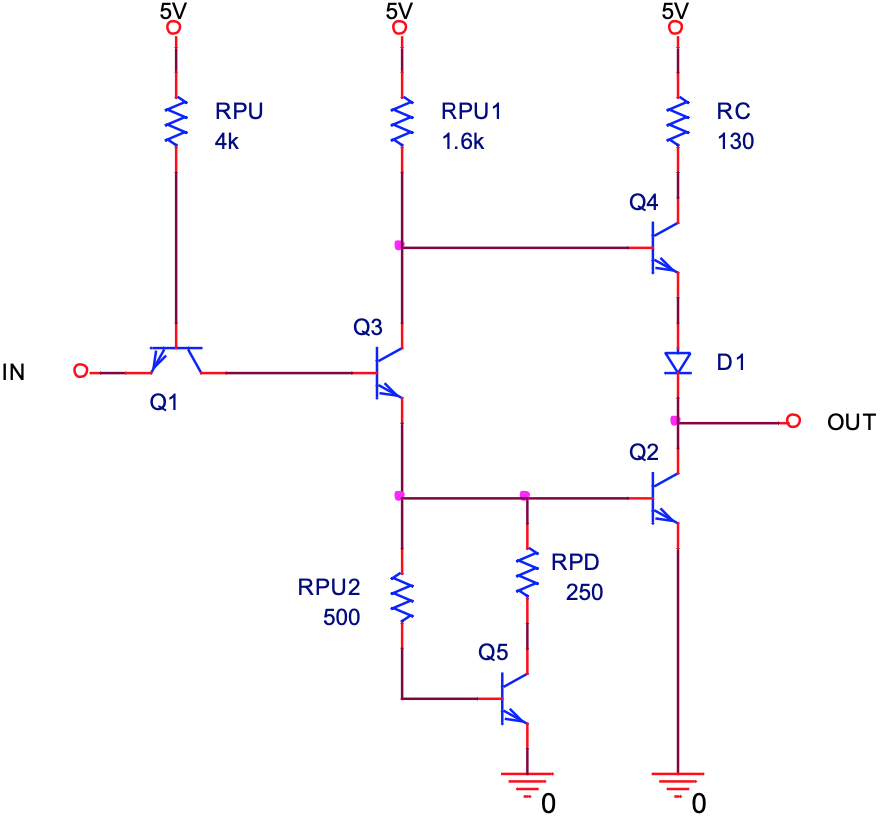
\includegraphics[scale=0.4,angle=0]{ttl_not_std.png}
    \caption{Struttura standard del NOT in logica TTL}
    \label{not_std}
\end{figure}

Le tre sezioni aggiunte all'interno del NOT standard rispetto alla struttura del NOT base sono così chiamate:
\begin{description}
    \item[Active Pull-Down APD] il circuito appena descritto, aggiunto per risolvere il problema della decrescita lineare della tensione di uscita. Viene chiamato così perché al suo interno è presente il transistor $Q_5$ che è un aggettivo attivo e ha il compito di sincronizzare il funzionamento di questa cella logica
    \item[Phase splitter] lo stadio intermedio composto dalle resistenze $R_{pu_1}$ e $R_{pd}$ e dal transistor $Q_3$. Viene così chiamato perché dato un ingresso (proveniente dal collettore del transistor $Q_1$) produce due uscite di fase opposta dirette alla base di $Q_4$ e $Q_2$
    \item[Totem-Pole] composto dai due transistor $Q_4$ e $Q_2$, dal diodo $D_1$ e dalla resistenza $R_c$.
\end{description}
Rifacendosi alla figura \ref{not_std} è possibile analizzare le sue caratteristiche principali:
\begin{itemize}
    \item Il transistor superiore di uscita $Q_4$ serve per guidare il circuito alto perché fornisce una piccola corrente tramite la quale l'uscita può essere tirata verso l'alto velocemente
    \item All'interno dell'APD, quando $Q_3$ si spegne il transistor $Q_5$ funge da raccoglitore di corrente perché la tensione che si trova sul nodo sottostante l'emettitore di $Q_3$ fa attivare la base di $Q_5$ che poi va ad assorbire corrente tramite la resistenza di pull-down $R_{pd}$
    \item La resistenza $R_c$ serve per limitare la cross conduzione di $Q_2$ e $Q_4$. L'inserimento dell'APD aiuta a sincronizzare tutte le varie operazioni
\end{itemize}

Con l'inserimento della sezione di active pull-down si risolve il problema della decrescita lineare della funzione di trasferimento che, come si vede in figura \ref{std_transfer}, perde completamente quella regione e la variazione della tensione in uscita diventa più repentino come effettivamente si vorrebbe nel contesto dell'elettronica digitale.
\begin{figure}[h]
    \centering
    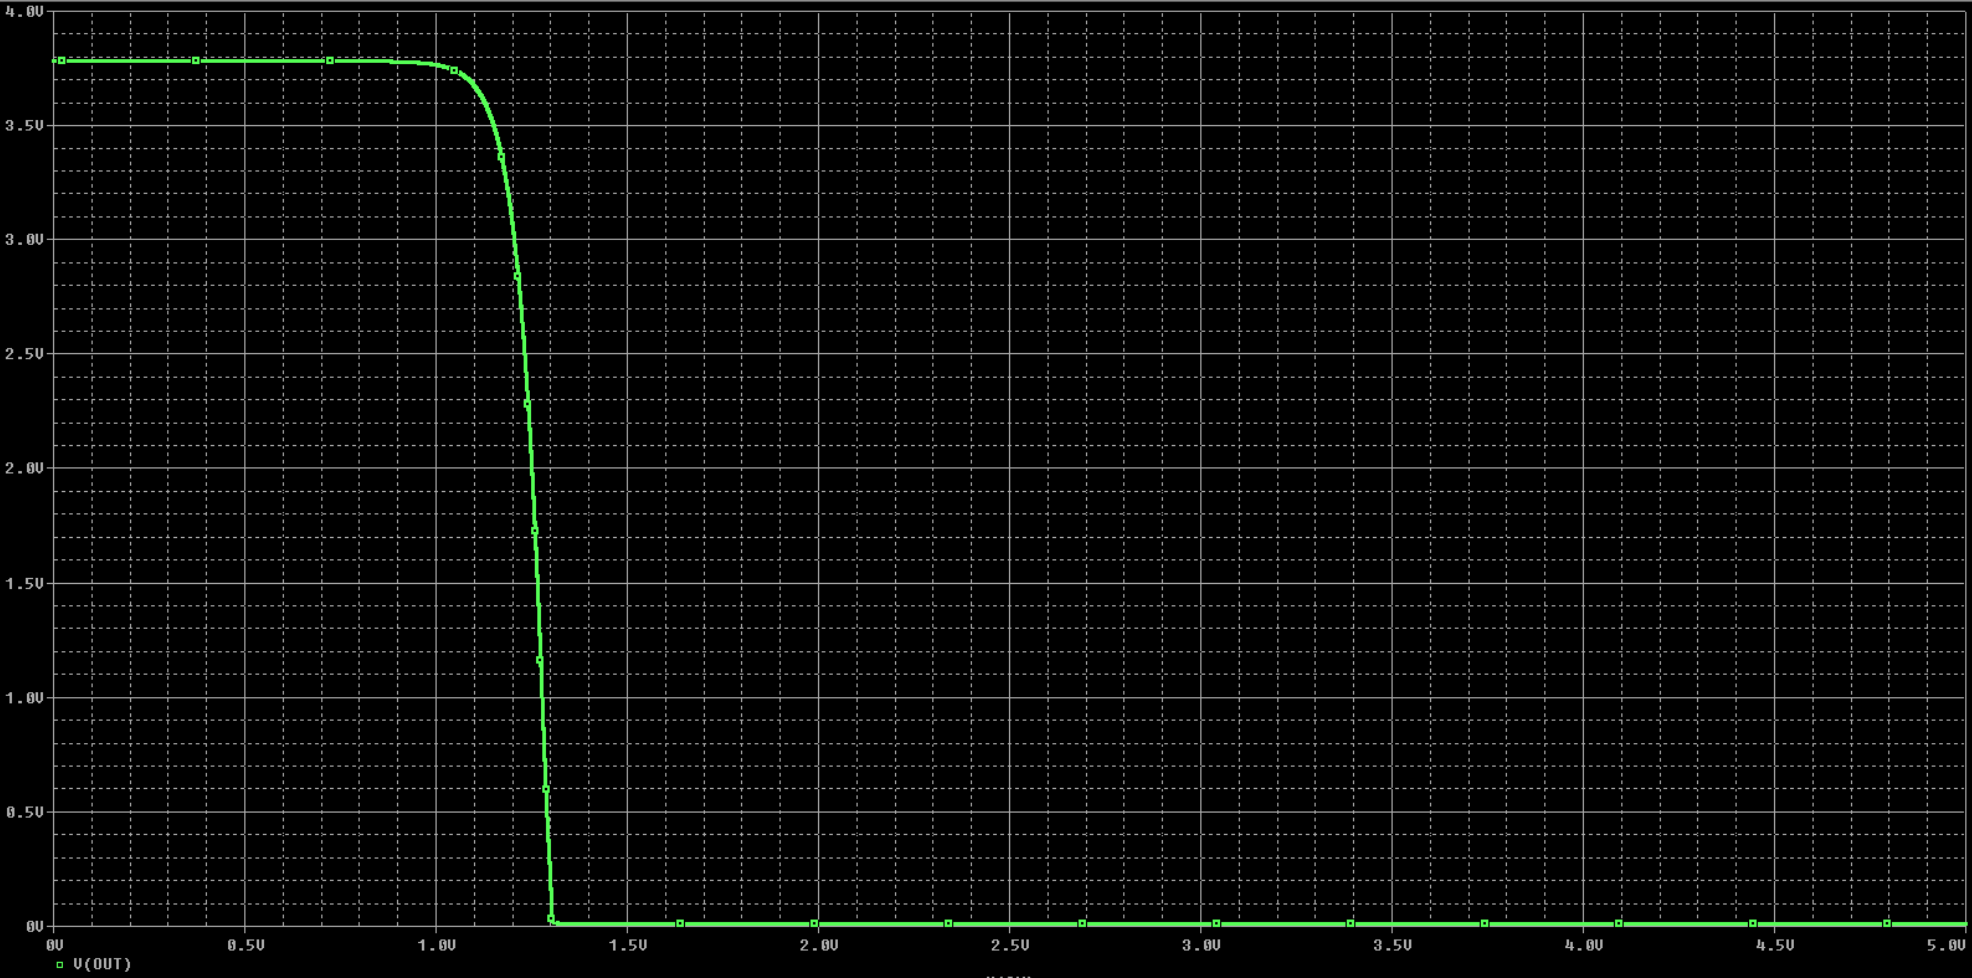
\includegraphics[scale=0.35,angle=0]{ttl_not_std_transfer.png}
    \caption{Tensione in uscita dal NOT standard}
    \label{std_transfer}
\end{figure}
\\Le decrescita lineare della tensione di uscita era dovuta al fatto che, dal momento in cui l'ingresso \textit{IN} era a $0,5\,V$, sul nodo sottostante l'emettitore di $Q_3$ iniziava a salire il potenziale che faceva scorrere una corrente all'interno dello stadio intermedio (composto da $R_{pu_{1}}$, $R_{pd}$ e $Q_3$). Con il nuovo circuito quando ci sono $0,5\,V$ in ingresso, e quindi anche sul collettore di $Q_1$, anche se la giunzione base-emettitore di $Q_3$ si accendesse per far passare un po' di corrente, tale corrente non potrebbe andare da nessuna parte perché tra l'emettitore di $Q_3$ e la resistenza $R_{pu_{2}}$ ci sono circa $0\,V$ e se si volesse far scorrere della corrente su $R_{pu_{2}}$ e su $R_{pd}$ in quel punto invece di avere circa $0\,V$ se ne dovrebbero avere almeno $0,7\,V$ perché si dovrebbe accendere $Q_5$. Dunque fino a circa $1,2 - 1,4\,V$ di tensione in ingresso che sta salendo, non succede niente. Nel momento in cui si raggiunge una tensione di $1,2 - 1,4\,V$, si accende $Q_5$ ma contemporaneamente si accende anche $Q_2$ perché su entrambi i transistor agisce una tensione di circa $0,6\,V$: il circuito è sincronizzato. Quando si accende $Q_5$, questo inizia pompare corrente, passante attraverso $R_{pu_{1}}$, tramite $R_{pd}$, quindi quando si accende $Q_5$ l'uscita tende ad abbassarsi. Contemporaneamente si accende anche $Q_2$ che tira l'uscita verso il basso.
\begin{figure}[h]
    \centering
    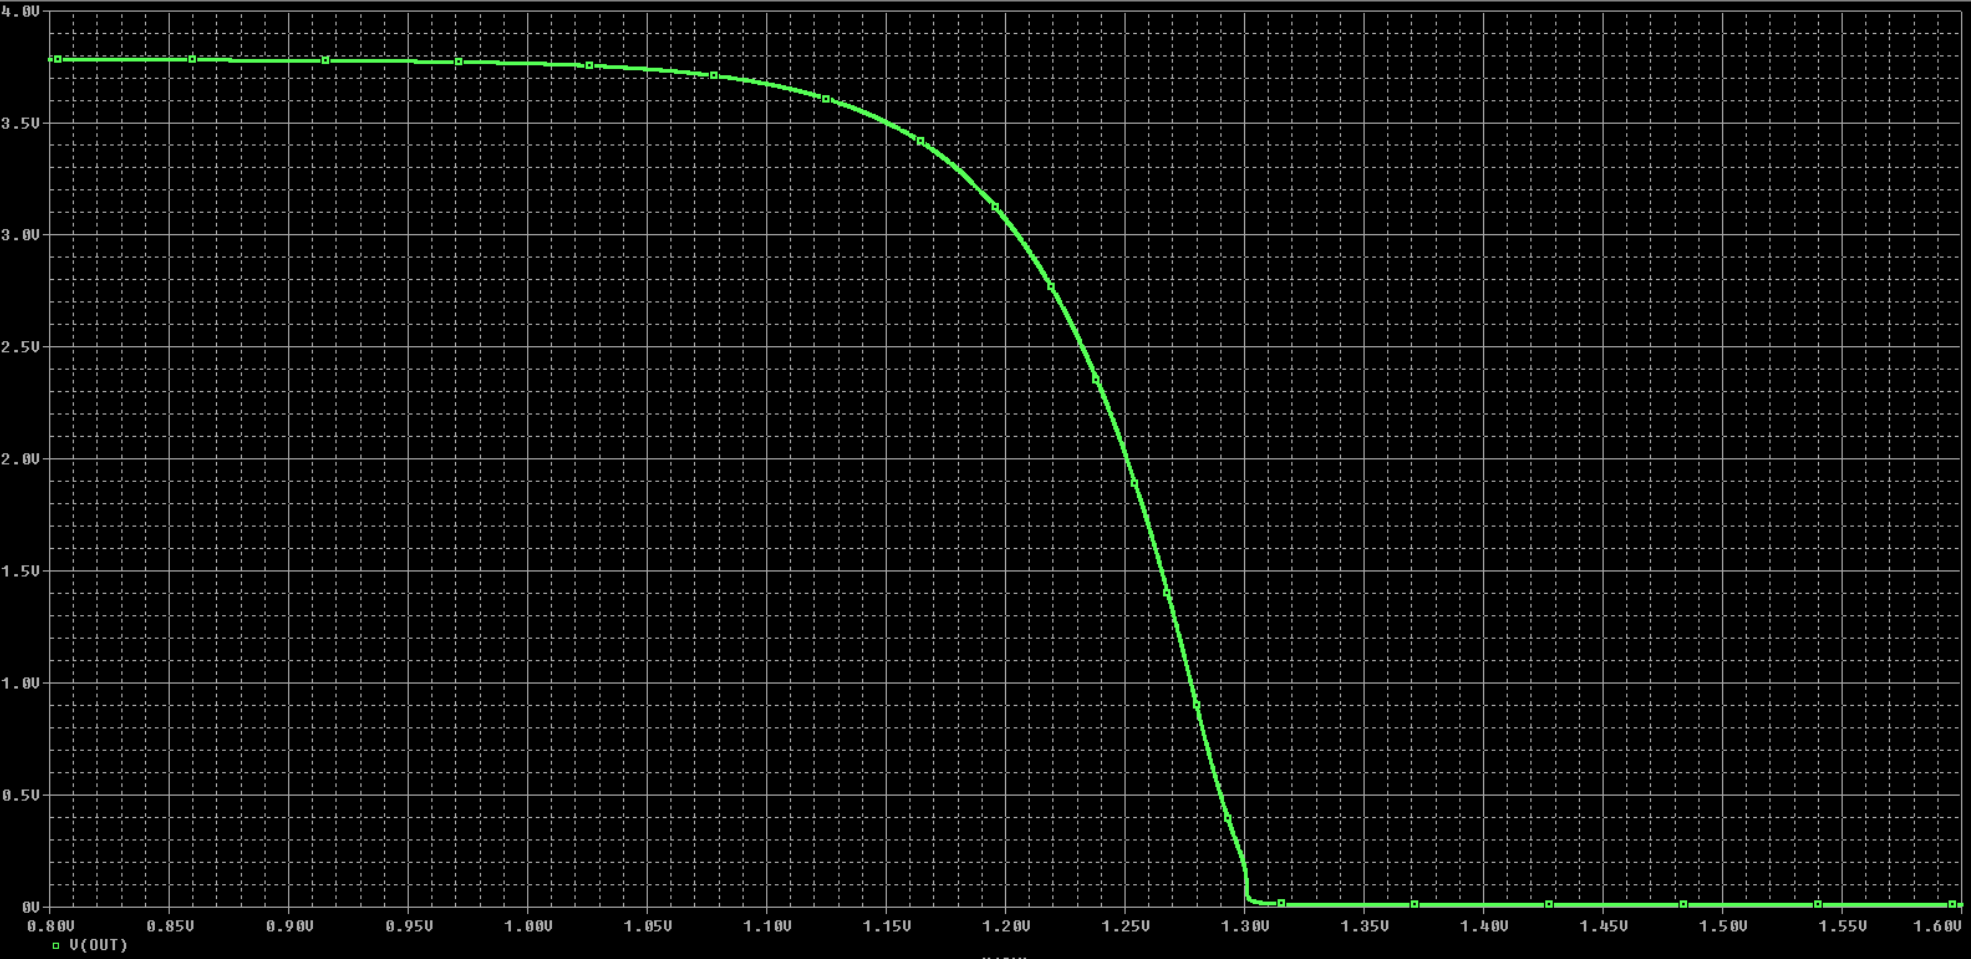
\includegraphics[scale=0.35,angle=0]{ttl_not_std_transfer_zoom.png}
    \caption{Zoom sulla regione di transizione}
    \label{std_zoom}
\end{figure}
\\La sincronizzazione delle azioni di $Q_2$ e $Q_5$ permette di abbassare repentinamente l'uscita del circuito in modo da evitare la regione lineare. Questa azione, come si nota nello zoom in figura \ref{std_zoom}, termina poi intorno a $1,4\,V$ in ingresso.

\section{Parametri della porta NOT standard}
\begin{itemize}
    \item Poiché la fase di decrescita repentina dell'uscita si conclude intorno a $1,35\,V$ si pone:
    \begin{equation}
        V_{iH} = 1,35\,V
    \end{equation}
    \item Al contrario, la medesima fase di decrescita inizia intorno a $1,1\,V$ in ingresso, dunque:
    \begin{equation}
        V_{iL} = 1,1\,V
    \end{equation}
    \item Per quanto riguarda la corrente in ingresso, si sa che $I_{iH}$ è determinata dalla corrente inversa che dipende dal funzionamento in regione attiva inversa del transistor $Q_1$. In questo caso la corrente inversa è molto bassa, circa l'1\,\% della corrente che scorre nel circuito:
    \begin{equation}
        I_{iH} \approx 15\,\mu A
    \end{equation}
    \item Quando invece la tensione in ingresso è bassa, come già detto nella \eqref{i_rpu}, per calcolare la corrente in ingresso si considera una tensione in ingresso di $0,2\,V$ e una tensione di $5\,V - 0,9\,V = 4,1\,V$ sulla resistenza di pull-up $R_{pu} = 4\,k\Omega$ per cui:
    \begin{equation}
        I_{iL} = \frac{5\,V - 0,9\,V}{4\,k\Omega} = \frac{4,1\,V}{4\,k\Omega} = 1\,mA
    \end{equation}
    \item La tensione di uscita alta, come già accennato nella \eqref{v_h}, vale:
    \begin{equation}
        V_{oH} = 3,75\,V
    \end{equation}
    e non può essere maggiore di questo valore perché in uscita ci sono il diodo $D_1$, su cui agisce una tensione di $0,7\,V$, e la giunzione base-emettitore di $Q_4$ su cui agiscono ancora $0,7\,V$. Quindi anche se si portasse la base di $Q_4$ a $5\,V$ tramite la resistenza $R_{pu_{1}}$, si avrebbe comunque una caduta di potenziale di $0,7\,V + 0,7\,V = 1,4\,V$.
    \item A tensione di uscita bassa, invece, la tensione di uscita è pari alla tensione di saturazione del transistor inferiore $Q_2$, dunque:
    \begin{equation}
        V_{oL} = 0,2\,V
    \end{equation}
\end{itemize}
A partire dai parametri statici è ora possibile ricavare il margine di rumore e la potenza dissipata:
\begin{itemize}
    \item Note le tensioni in ingresso e in uscita per i due livelli logici, si calcolano il margine di rumore alto e basso:
    \begin{equation*}
        \textit{NM}_{H} = V_{oH} - V_{iH} = 3,75\,V - 1,35\,V = 2,4\,V
    \end{equation*}
    abbastanza alto
    \begin{equation*}
        \textit{NM}_{L} = V_{iL} - V_{oL} = 1,1\,V - 0,2\,V = 0,9\,V
    \end{equation*}
    l'aver aggiunto tutti i transistor intermedi ha fatto salire la $V_{iL}$ e questo è positivo per la porta logica perché il rumore elettrico è ora più alto. Segue quindi il rumore elettrico:
    \begin{equation}
        \textit{NM} = min(\textit{NM}_{L},\, \textit{NM}_{H}) = 0,9\,V
    \end{equation}
    \item Per quanto riguarda la potenza, non si può più dire che la potenza alta e bassa sono uguali né che una delle due è nulla perché ci sono così tante componenti che ci sarà sempre un qualche ramo che consuma della corrente. Quando l'uscita è bassa i transistor $Q_2$ e $Q_3$ sono entrambi accesi, quindi la corrente scorre nelle resistenze $R_{pu}$ e $R_{pu_{1}}$. Poiché il potenziale dell'emettitore di $Q_2$ è di $0\,V$, tra la base di $Q_2$ e l'emettitore di $Q_3$ ci sono $0,7\,V$, tra la base di $Q_3$ e il collettore di $Q_1$ ci sono $1,4\,V$ e sulla base di $Q_1$ ci sono circa $2,1\,V$, si può calcolare la corrente che scorre attraverso $R_{pu}$
    \begin{equation*}
        I_{R_{pu}} = \frac{5\,V - 2,1\,V}{4\,k\Omega} \approx 0,7\,mA
    \end{equation*}
    (dunque $Q_3$ è in saturazione) e la corrente che scorre attraverso $R_{pu_{1}}$
    \begin{equation*}
        I_{R_{pu_{1}}} = \frac{5\,V - 0,9\,V}{1,6\,k\Omega} \approx 2,5\,mA
    \end{equation*}
    In base a queste informazioni si ottiene:
    \begin{equation*}
        P_{L} = 5\,V \cdot (0,7\,mA + 2,5\,mA) = 16\,mW
    \end{equation*}
    Quando invece l'uscita è alta l'unica componente in cui scorre corrente è la resistenza di ingresso $R_{pu}$ per cui
    \begin{equation*}
        P_{H} = 5\,V \cdot 1\,mA = 5\,mW
    \end{equation*}
    Infine, la potenza media è data da:
    \begin{equation}
        P = \frac{P_{L} + P_{H}}{2} = \frac{16\,mW + 5\,mW}{2} \approx 11,5\,mW
    \end{equation}
\end{itemize}

\subsection{Parametri dinamici}
Quando si deve passare dal livello logico alto a basso sono sufficienti pochi nanosecondi (circa $5\,nS$) perché per effettuare questo passaggio si deve accendere il transistor $Q_2$ (come nel caso del NOT RTL) che è un'operazione veloce. In questo caso non ci si preoccupa di spegnere il transistor superiore del totem pole, cioè $Q_4$, perché deve spegnersi più tardi e ciò che conta è che il nodo tra $R_{pu_{1}}$ e la base di $Q_4$, che è a $0,9\,V$, viene portato giù dalla corrente che scorre attraverso $R_{pu_{1}}$.

Analogamente, nel passare dal livello logico basso a quello alto il transistor $Q_2$ deve essere spento e per farlo si devono rimuovere le cariche minoritarie al suo interno. È qui che entra il gioco la sezione di active pull-down composta dal transistor $Q_5$ che consente ti rendere tutta questa operazione veloce. A differenza del passaggio di livello precedente, in questo $Q_4$ deve essere spento e per farlo entra in gioco $Q_5$. Anche in questo caso sono sufficienti circa $5\,nS$. 

Per quanto detto, i tempi di propagazione $t_{p_{HL}}$ e $t_{p_{LH}}$ sono:
\begin{equation}
    t_{p_{HL}} \approx 5\,nS \text{ \, \, } t_{p_{LH}} \approx 5\,nS
\end{equation}
Ricordando che la potenza dissipata è circa $11\,mW$ (quasi la metà rispetto al caso RTL), si può calcolare il prodotto ritardo-potenza (più piccolo è e meglio è perché significa che si ha poco ritardo e/o poco consumo):
\begin{equation}
    \textit{DP} = t_{p} \cdot P = 5\,nS \cdot 11,5\,mW = 57,5\,pJ
\end{equation}
circa $2/3$ di quello della porta logica NOT nella famiglia RTL.
\section{NAND}
Data la porta NOT, il componente più adatto da affiancare a tale porta logica per poter effettivamente ottenere una famiglia logica in grado di implementare una qualsiasi funzione logica è la porta \textbf{NAND}. La scelta di questa porta logica è dovuta al fatto che è possibile realizzare \textbf{transistor multiemettitore} il cui funzionamento è del tutto analogo a quello del transistor tradizionale con la sola differenza che la corrente che scorre in una delle due giunzioni base-emettitore1 o base-emettitore2 è indifferente. Con questo transistor, qualsiasi dei due ingressi venga messo \textit{basso} fa considerare l'ingresso come \textit{basso}, il resto del circuito è esattamente uguale al circuito della porta NOT.

Se uno dei due ingressi è \textit{basso}, polarizza \textit{direttamente} la giunzione tra la base e l'emettitore (l'altro ingresso invece di rimanere basso è disattivato, cioè non ci scorre corrente ed è come se non ci fosse) e quindi la fa considerare come un ingresso basso permettendo di avere l'uscita del circuito \textit{alta} (il NAND è vero e almeno uno dei due ingresso è falso).

Viceversa, se entrambi gli ingressi sono \textit{alti} è come se si avesse un solo emettitore alto e a quel punto l'ingresso è effettivamente considerato come \textit{alto} e l'uscita del circuito è \textit{bassa}.

Se non è presente la sezione di active pull-up (cioè mancano la resistenza $R_c$ il transistor $Q_4$ e il diodo $D_1$) il circuito viene chiamato \textbf{open collector} e l'uscita è composta solo dal transistor $Q_2$. Per poter utilizzare l'uscita del circuito si dovrà inserire esternamente una resistenza di pull-up così il circuito torna ad essere uguale allo stadio di uscita della porta NOT in versione RTL. Questa tipologia di circuiti, insieme alla classe \textbf{open drain} nel caso dei circuiti C-MOS, ha una serie di possibili applicazioni, un esempio è la possibilità di modificare la tensione di uscita della porta logica: si vuole cioè porre il pull-up ad una tensione desiderata diversa dai canonici $5\,V$.
\begin{figure}[ht]
    \centering
    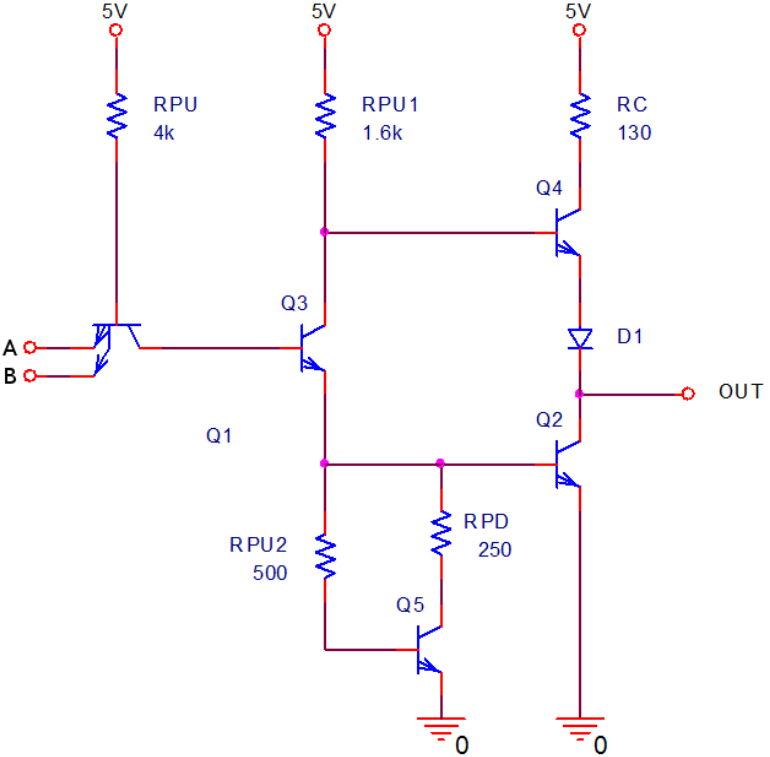
\includegraphics[scale=0.4,angle=0]{ttl_nand.png}
    \caption{Struttura del NAND in logica TTL}
    \label{ttl_nand}
\end{figure}

\section{Comportamento dinamico del NOT}
Si vuole studiare cosa succede all'interno del circuito quando l'ingresso, e conseguentemente anche l'uscita, cambia stato ovvero quando esegue la commutazione. Si considera la versione \textit{standard} della porta NOT in logica TTl.

\subsection{Commutazione dell'uscita $H \rightarrow L$}
Inizialmente l'uscita è alta e l'ingresso è basso ma ad un certo punto l'ingresso passa ad essere alto e si vuole studiare cosa succede a livello dinamico all'interno del circuito. 

Quando l'ingresso è \textit{basso} significa che su \textit{IN} ci sono circa $0\,V$ e quindi $Q_1$ ha la giunzione tra base ed emettitore polarizzata \textit{direttamente} dalla resistenza di pull-up $R_{pu}$. Di conseguenza, poiché tra la base di $Q_3$ e il collettore di $Q_1$ non scorre corrente diretta verso $Q_1$ se non quella di rimozione delle cariche, la corrente di collettore in condizioni statiche è $I_{c} \approx 0\,A$ quindi si può supporre che $Q_1$ è in \textit{saturazione} e, nelle medesime condizioni, $Q_3$ è \textit{spento}. Poiché $Q_3$ è spento nel nodo sottostante il suo emettitore ci sono circa $0\,V$ e quindi anche $Q_5$ e $Q_2$ sono \textit{spenti}. Rimane solo $Q_4$ nella cui base scorre una corrente grazie a $R_{pu_{1}}$ e sul suo collettore è presente una tensione data da $I \cdot R_c$ dunque, in condizioni normali (quando la corrente che scorre nella sua base è modesta), $Q_4$ lo si considera in regione \textit{attiva}.

Quando invece l'ingresso commuta passando ad essere \textit{alto} si ottiene che i transistor $Q_2$, $Q_3$ e $Q_5$ sono in \textit{saturazione} mentre $Q_4$ è \textit{spento} e $Q_1$ è in regione \textit{attiva inversa}.

Tuttavia, per poter arrivare in questa configurazione, sicuramente $Q_1$ e $Q_4$ dovranno spegnersi mentre $Q_2$, $Q_3$ e $Q_5$ dovranno accendersi. Andando nel dettaglio, durante la commutazione dell'uscita dovuta alla variazione dell'ingresso, per prima cosa $Q_1$ passa dalla saturazione alla regione attiva inversa perché mano a mano che aumenta l'ingresso, la tensione $V_{be}$ diventa nulla così il transistor sarà momentaneamente in interdizione e poi regione attiva inversa. Non appena $Q_1$ entra in regione attiva inversa e grazie al pull-down attivo si attivano insieme $Q_2$, $Q_3$ e $Q_5$ e, ancora contemporaneamente, $Q_4$ si spegne. Come si vede in figura \ref{h_to_l}, poiché $Q_4$ non era in saturazione, il suo spegnimento è più facile e regolare rispetto allo spegnimento di un transistor in piena saturazione.
\begin{figure}[ht]
    \centering
    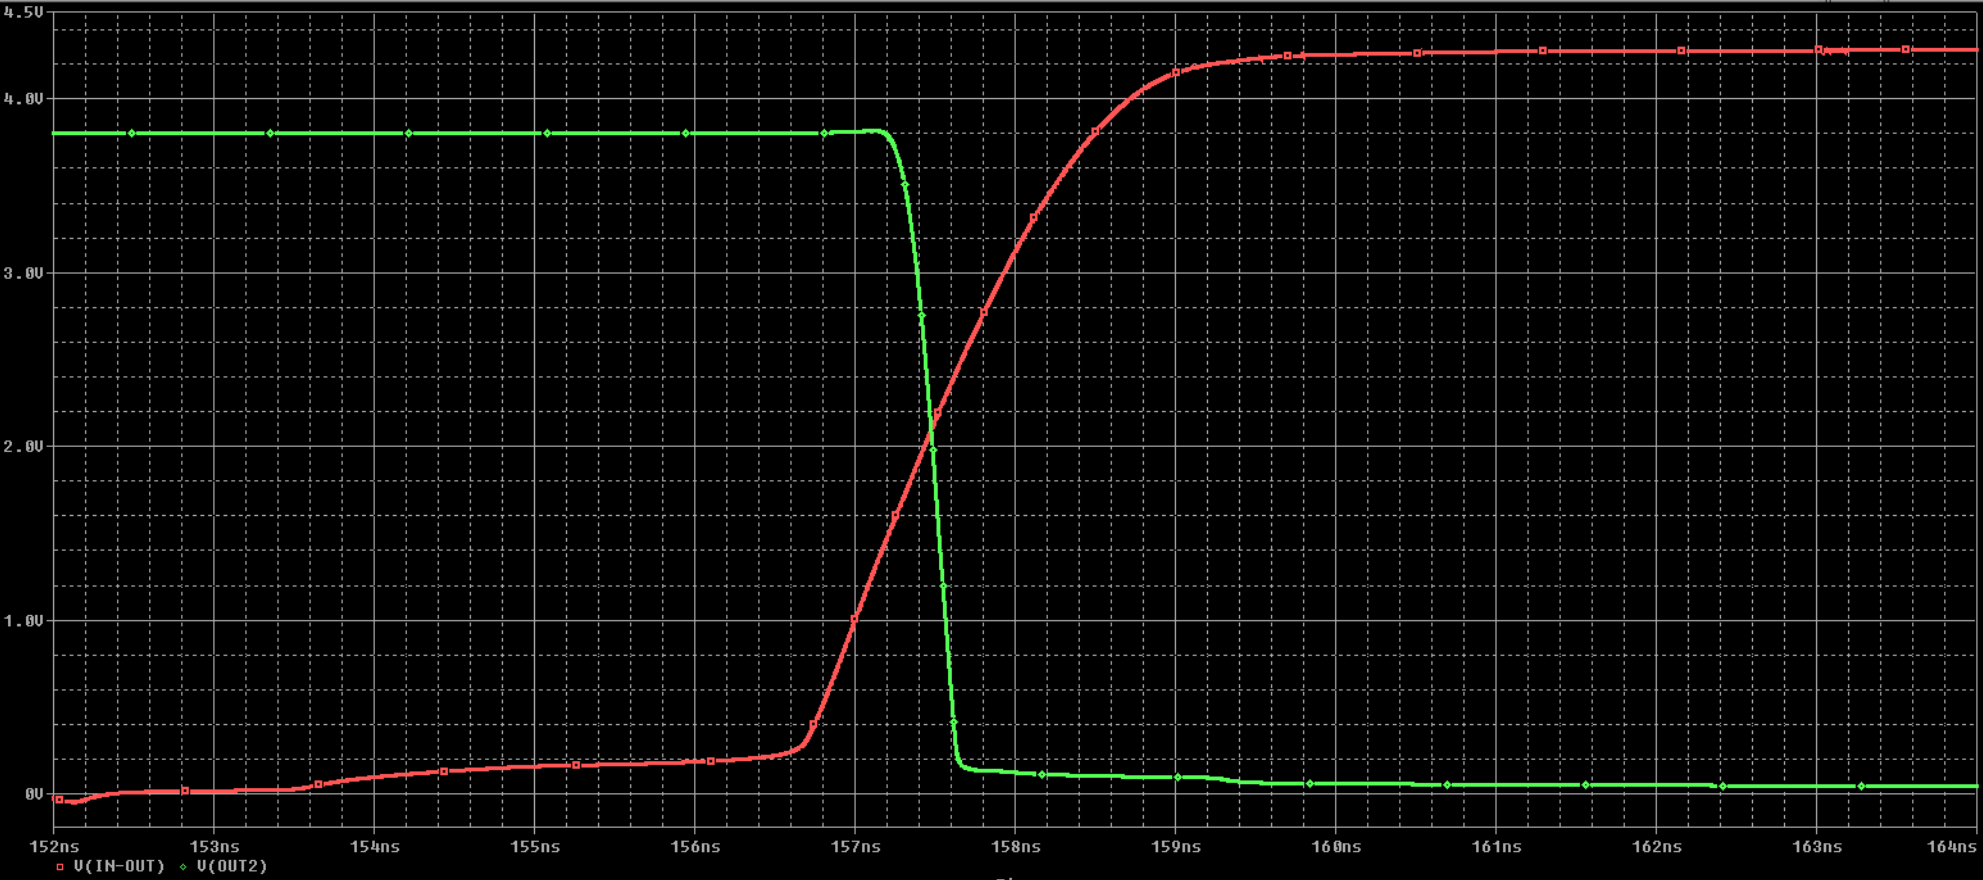
\includegraphics[scale=0.35,angle=0]{ttl_h_to_l.png}
    \caption{Commutazione $H \rightarrow L$}
    \label{h_to_l}
\end{figure}
\\Dalla figura \ref{h_to_l} si nota che l'uscita inizia a passare a livello logica basso in corrispondenza di circa $1,5\,V$ (grazie alla sincronizzazione del circuito per tensioni minori non succede niente). Per valori di tensioni maggiori grazie all'accensione dei tre transistors $Q_2$, $Q_3$ e $Q_5$ si ha una variazione abbastanza repentina dell'uscita. In corrispondenza di ciò l'ingresso invece passa lentamente al livello logico alto. Questo maggior lentezza rispetto alla velocità con cui varia l'uscita è dovuto al fatto che lo stadio TTL è composto dal diodo $D_1$ con $Q_4$ e $R_c$ che rallentano la variazione.

In questa commutazione dell'uscita non ci sono criticità rilevanti: non appena viene superata la tensione di soglia $V_{iH} = 1,4\,V$ l'uscita commuta immediatamente e in meno di un nanosecondo l'uscita si è già stabilizzata sul livello logico basso. Questa elevata velocità di commutazione è dovuta al fatto che quasi l'intersa fase di commutazione è dovuta all'accensione dei tre transistors e lo spegnimento di uno solo che, come già detto, è abbastanza rapido.

\subsection{Commutazione dell'uscita $L \rightarrow H$}
Inizialmente l'uscita è bassa e l'ingresso è alto ma ad un certo punto l'ingresso passa al livello logico basso.

Quando l'ingresso è \textit{alto} i tre transistors $Q_2$, $Q_3$ e $Q_5$ sono accesi e si trovano in \textit{saturazione} ma dopo che l'ingresso è diventato \textit{basso} ci si trova nella situazione iniziale del caso precedente ovvero $Q_1$ è in \textit{saturazione} e $Q_4$ è acceso e si trova in regione \textit{attiva diretta}. L'accensione e lo spegnimento di $Q_4$ non sono operazioni rilevanti dal punto di vista della complessità e anche il passaggio di $Q_1$ da regione attiva inversa alla regione di saturazione è un passaggio ugualmente semplice. Ciò che si deve fare affinché la commutazione sia completa è spegnere i tre transistors accesi e tutti in saturazione: questa operazione è invece molto complessa.

Per prima cosa, in seguito alla variazione dell'ingresso, $Q_1$ passa da attiva inversa ad attiva diretta per un brevissimo periodo di tempo per poi finire in saturazione. Il breve intervallo in attiva diretta è dovuto al fatto che quando l'ingresso è alto sul suo collettore ci sono $1,4\,V$ e quando l'ingresso viene portato a $0\,V$ la giunzione tra base ed emettitore si polarizza subito ma sull'emettitore continuerà a persistere $1,4\,V$ perché ci sono le cariche accumulate e delle capacità parassite per cui $Q_1$ dovrà estrarre delle cariche da $Q_3$, spegnendolo, e per farlo scorrerà una corrente dal collettore all'emettitore, quindi sarà in attiva diretta. Non appena $Q_3$ inizia a spegnersi ed entrare in saturazione si attiva tutta la parta destra del circuito.

Il funzionamento di tale parte dipende però da quale tipologia di porta NOT si considera, infatti nelle versioni viste può essere presente o meno la zona di pull-down attivo ($Q_5$, $R_{pd}$ e $R_{pu_{2}}$) e inoltre può anche essere eventualmente sostituita con una zona di pull-down \textit{resistivo} (cioè una sola resistenza).

\subsubsection{$L \rightarrow H$ senza APD}
Se non è presente la zona di active pull-down tra i transistors $Q_3$ e $Q_2$ c'è una semplice resistenza $R_{pd}$.
\begin{figure}[h]
    \centering
    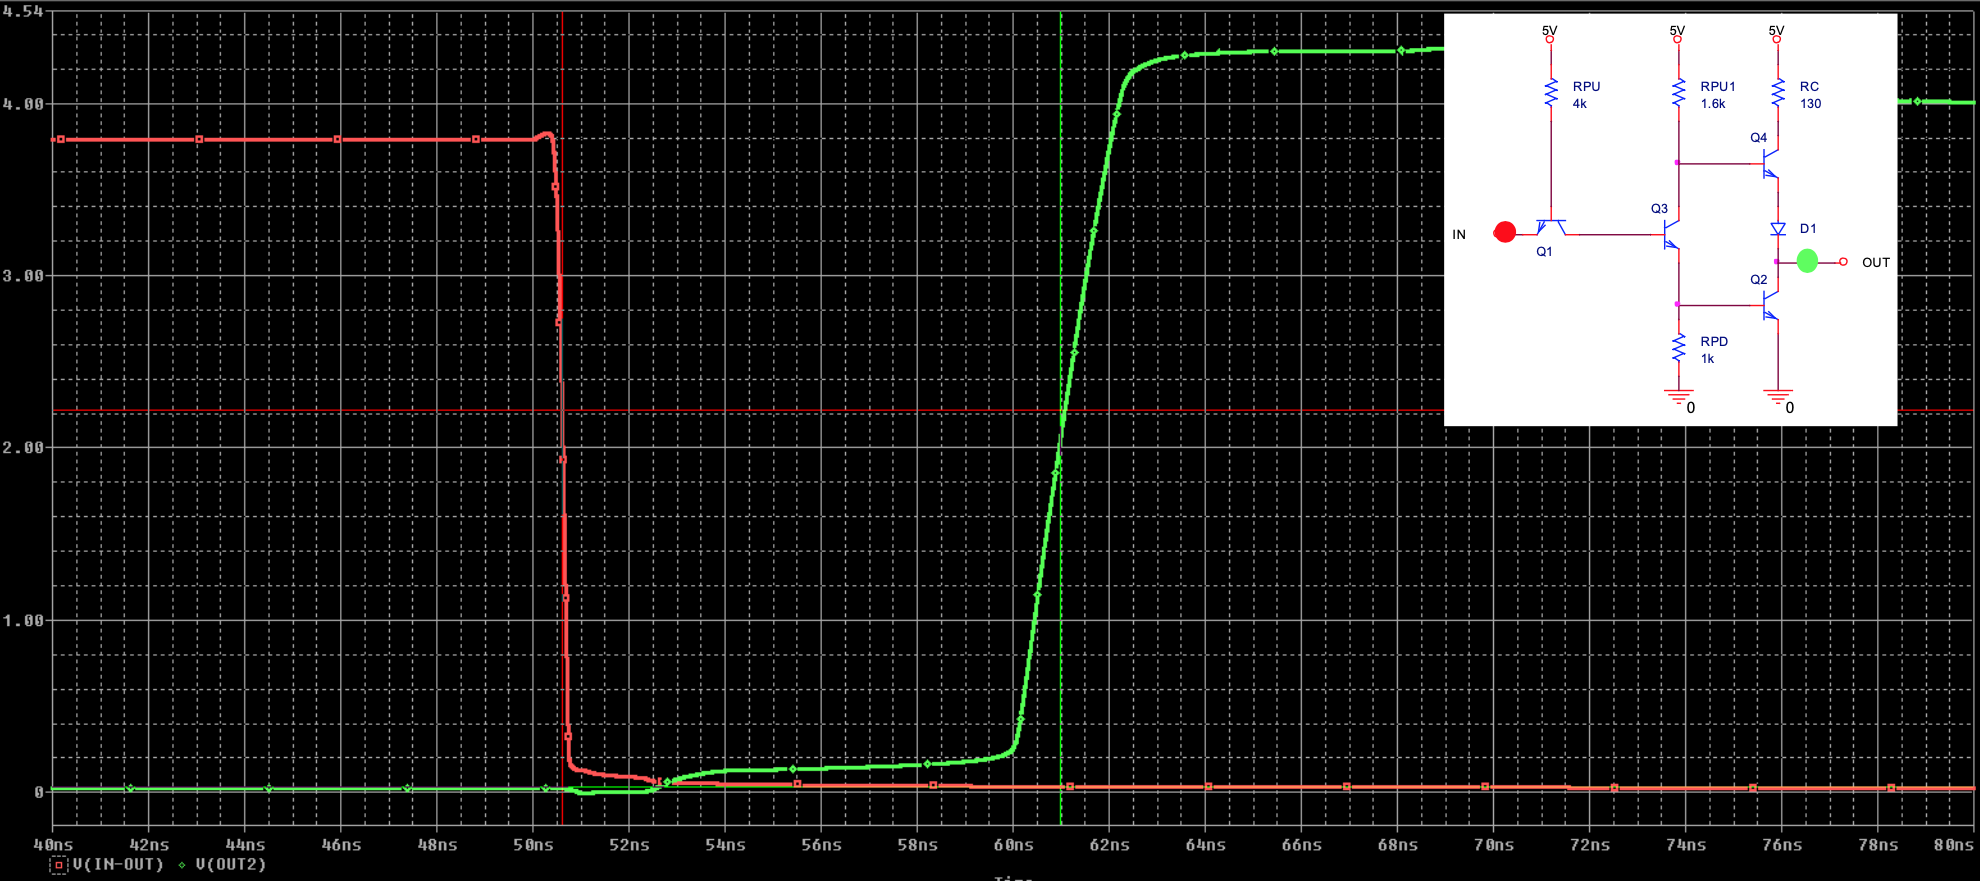
\includegraphics[scale=0.35,angle=0]{ttl_l_to_h_noapd1.png}
    \caption{Commutazione $L \rightarrow H$ senza APD}
\end{figure}
\\L'ingresso commuta rapidamente passando dal livello logico alto a quello basso, al contrario l'uscita non cambia più istantaneamente come nel caso precedente ma cambia dopo un intervallo temporale di circa $10\,nS$. Durante questo intervallo l'uscita, dopo essere rimasta inizialmente invariata, fa un primo modesto salto di tensione, rimane poi circa costante e infine subisce un'impennata verso l'alto.

Il primo intervallo temporale in cui l'uscita rimane invariata indica il tempo necessario a $Q_1$ per poter svuotare la base di $Q_3$ spegnendolo. Nel momento in cui $Q_3$ si spegne non passa più corrente né in $R_{pu_{1}}$ né in $R_{pd}$ e questo fa sì che scorra corrente in $Q_4$ che si accende e tenta di tirare l'uscita verso l'alto realizzando quel piccolo salto. Tuttavia $Q_2$ deve ancora spegnersi perché era in saturazione e l'unico modo per farlo è attraverso la poca corrente che può essere scaricata tramite $R_{pd}$. Quindi la fase in cui l'uscita rimane quasi costante si verifica perché $Q_2$ si sta spegnendo. Non appena $Q_2$ si è spenta si ha lo scatto verso l'alto dell'uscita tirata dal blocco alto del totem pole ($D_1$, $Q_4$ e $R_c$).

Nella fase in cui l'uscita rimane quasi costante è attivo sia il blocco alto che quello basso del totem pole, questo lo si può vedere analizzando l'assorbimento di corrente della porta logica come riportato in figura \ref{l_to_h1}. Nell'intervallo di tempo compreso tra quando l'ingresso commuta e $Q_3$ si spegne s $Q_4$ si accende l'assorbimento di corrente rimane costante. Non appena si accende $Q_4$ esso inizia a pompare corrente che scorre all'interno di tutto il totem pole, quindi l'assorbimento di corrente impenna verso l'alto stabilizzandosi su un valore di $30\,mA$ che dipende dalla resistenza $R_c$. Si nota dunque che commutare l'uscita dal livello logico basso a quello alto consuma un'energia di
\begin{equation*}
    6\,nS \cdot (5\,V \cdot 30\,mA) = 6\,nS \cdot 150\,mW = 900\,pJ
\end{equation*}
che, essendo tanta, non è trascurabile e non si può far commutare tante volte la porta logica perché per ogni commutazione sono appunto consumati $900\,pJ$. 
\begin{figure}[ht]
    \centering
    \includegraphics[scale=0.35,angle=0]{ttl_l_to_h_noapd2.png}
    \caption{Assorbimento di corrente nella commutazione $L \rightarrow H$ senza APD}
    \label{l_to_h1}
\end{figure}

\subsubsection{$L \rightarrow H$ con APD}
Il pull-down attivo si basa sulla sincronizzazione, sia in accensione che in spegnimento, di $Q_2$, $Q_3$ e $Q_5$ e in particolare permette uno spegnimento rapido e facile.
\begin{figure}[h]
    \centering
    \includegraphics[scale=0.35,angle=0]{ttl_l_to_h_apd1.png}
    \caption{Commutazione $L \rightarrow H$ con APD}
\end{figure}
\\Anche in questo caso l'ingresso va giù molto velocemente e dopo un paio di nanosecondi la base di $Q_3$ è svuotata. A questo punto si accende $Q_4$ e si spegne $Q_2$. Rispetto al caso precedente la presenza di $Q_5$ nel carico attivo permette di ridurre il tempo necessario per spegnere $Q_2$ a pochi nanosecondi (è stato dimezzato circa) perché è in grado di tirare corrente molto velocemente.

Analizzando l'assorbimento di corrente durante la commutazione dell'uscita riportato in figura \ref{l_to_h2} si nota che la regione d'interesse è molto più ristretta rispetto al caso precedente. Utilizzando l'APD si è riuscito a dimezzare il consumo di energia che continua però ad avere lo stesso andamento. L'energia di commutazione è più che minore della metà di quella del caso precedente in cui non viene utilizzato il pull-down attivo. Inoltre il passaggio $L \rightarrow H$ è molto più veloce perché si passa da $10\,nS$ a circa $5\,nS$ quindi è stato \textit{dimezzato} anche il tempo di propagazione. Il circuito, oltre ad essere più veloce è anche più efficiente dal punto di vista energetico.
\begin{figure}[ht]
    \centering
    \includegraphics[scale=0.35,angle=0]{ttl_l_to_h_apd2.png}
    \caption{Assorbimento di corrente nella commutazione $L \rightarrow H$ con APD}
    \label{l_to_h2}
\end{figure}

\chapter{CMOS e BiCMOS}
I transistors N-MOS e P-MOS prendono il nome di \textbf{MOS ad arricchimento} perché per creare il canale di conduzione, tale canale deve essere arricchito di cariche portatrici; quindi un MOS a canale n deve essere arricchito di elettroni mentre uno a canale p di lacune.

Oltre a questa categoria, ne esiste una seconda chiamata \textbf{MOS a svuotamento} carattierizzati dal fatto che, in fase di costruzione, tra source e drain viene creata una zona drogata n+ in modo da formare nativamente un canale che li connette direttamente. Se non viene applicata tensione al gate, il canale è già esistente quindi in condizioni normali c'è conduzione tra source e drain. L'unica operazione possibile è spegnerlo attivamente. Per farlo si abbassa la tensione di gate $V_{gs}$ (come nel caso di uno ad arricchimento in cui si tolgono le cariche portatrici) facendola diventare negativa in modo che inizi ad attrarre cariche positive al di sotto del canale, queste vanno a neutralizzare la zona n+ fino a farla diventare una zona p chiudendo così il canale di conduzione.

A livello pratico il MOS a svuotamento ha la stesse equazioni viste per quello ad arricchimento con la vola differenza che la tensione di soglia $V_t$ è \textit{negativa} e dunque anche semplicemente con $V_{gs} = 0\,V$ la tensione di soglia è già stata superata e quindi il dispositivo è acceso in conduzione. Per spegnerlo si deve avere $V_{gs} < V_{t} < 0\,V$.

\section{CMOS}
Il termine indica la famiglia delle porte MOS \textbf{complementari} così chiamate per indicare il fatto che si utilizza un dispositivo a canale p e un complementare dispositivo a canale n. Generalmente, per ragioni di simmetria, si vuole che questi due dispositivi siano uguali a livello di comportamente e prestazioni.

\subsection{NOT}
Come si vede in figura \ref{cmos} l'implementazione in logica CMOS della porta logica NOT è composta da due transistors: uno a canale p nella parte superiore e uno a canale n nella parte inferiore.

Quando l'ingresso $V_{i}$ del circuito è \textit{alto}, la $V_{gs}$ di $Q_n$ è alta quindi si suppone che $Q_n$ sia acceso e si trovi in regione \textit{lineare} e in questo condizioni il transistor viene visto come la corrispondente resistenza di canale $R_{dsn}$. Al contrario, la $V_{gs}$ di $Q_p$ è circa $0\,V$ quindi il transistor è \textit{spento} ed è come se nella parte alta dell'intero circuito non ci fosse niente. Dunque, quando l'ingresso è alto si vede solo la resistenza del MOS a canale n che tira l'uscita verso il basso, dunque il livello logico in uscita è \textit{basso}.

Viceversa, se l'ingresso è \textit{basso}, la $V_{gs}$ di $Q_n$ è circa $0\,V$ mentre quella di $Q_p$ è circa $-V_{dd}$ (la tensione di soglia di un P-MOS è negativa), in questa condizione il transistor a canale n è \textit{spento}, quindi non c'è la parte inferiore del circuito, mentre quello a canale p è acceso e si trova in regione \textit{lineare}. Nel complesso, si vede solo la resistenza di canale $V_{dsp}$ del P-MOS che fa sì che l'uscita del circuito sia \textit{alta}.
\begin{figure}[h]
    \centering
    \includegraphics[scale=0.4,angle=0]{cmos.png}
    \caption{Struttura di un CMOS \textit{inverter}}
    \label{cmos}
\end{figure}
\\Nel funzionamento della porta NOT si vedono \textit{alternativamente} i due dispositivi complementari. Inoltre, se il dispositivo è esattamente simmetrico la curva di tensione del dispositivo è \textit{simmetrica} rispetto a metà tensione di alimentazione e questo permetterà di aumentare, massimizzandoli, i margini di rumore.

Per determinare come varia l'uscita rispetto all'ingresso si hanno a disposizione solo informazioni relative alla corrente di drain $I_{d}$ che si sa essere definita come:
\begin{equation}
    I_{d} = K\,[2(V_{gs} - V_{t})V_{ds} - V_{ds}^2]
    \label{i_d}
\end{equation}
ma ciò che si vuole studiare è invece $V_{o}$ dunque la prima cosa che si deve fare è stabilire come ricavare la tensione di uscita partendo dalla corrente di drain. La prima assunzione che si fa è che tutta la corrente del transistor a canale p, cioè $I_{d_{p}}$, passa nel secondo transistor a canale n, per cui:
\begin{equation}
    I_{d_{p}} = I_{d_{n}}
    \label{i_cmos}
\end{equation}
Questa assunzione è vera perché l'uscita, che si suppone vada a guidare un'altra porta logica dello stesso tipo, non assorbe corrente. I dispositivi MOS ha l'ingresso controllato in tensione dunque, poiché il gate è isolato (è un condensatore), in condizioni statiche non scorre corrente nel gate e dunque, sempre in condizioni statiche, alla porta logica CMOS non viene richiesta corrente. In condizioni statiche la corrente di uscita è $I_{o} \approx 0\,A$ e questo comporta la validità del \eqref{i_cmos}. In particolare, la \eqref{i_d} varia per i due transistor perché sono diverse le relative tensioni $V_{ds}$ e $V_{gs}$ e cambia anche \textit{K} definito come:
\begin{equation*}
    K_{p} = \frac{1}{2}\mu_{p} C_{ox}\frac{W_p}{L_p}
\end{equation*}
\begin{equation*}
    K_{n} = \frac{1}{2}\mu_{n} C_{ox}\frac{W_n}{L_n}
\end{equation*}
Si ricavano due correnti di drain che, come detto nella \eqref{i_cmos}, devono essere uguagliate. Nell'equazione che definisce la corrente di drain per il MOS a canale n, cioè $I_{d_{n}}$, la $V_{ds}$ corrisponde a $V_{o}$:
\begin{equation}
    V_{ds_{n}} = V_{o}
\end{equation}
quella che si vuole trovare, mentre $V_{gs}$ corrisponde a $V_{in}$: 
\begin{equation}
    V_{gs_{n}} = V_{i}
\end{equation}
Per quello a canale p la situazione è leggermente diversa perché valgono:
\begin{equation}
    V_{ds_{p}} = V_{dd} - V_{o}
\end{equation}
\begin{equation}
    V_{gs_{p}} = V_{dd} - V_{i}
\end{equation}
Sostituendo questi valori all'interno delle equazioni dei due dispositivi ed eguagliandole per la \eqref{i_cmos}, si ricava la tensione $V_{o}$ e il suo andamento rispetto $V_i$:
\begin{equation*}
    \frac{1}{2}\mu_{p} C_{ox}\frac{W_p}{L_p}\,[2(V_{dd} - V_{i} - V_{t})(V_{dd} - V_{o}) - (V_{dd} - V_{o})^2] = \frac{1}{2}\mu_{n} C_{ox}\frac{W_n}{L_n}\,[2(V_{i} - V_{t})V_{o} - V_{o}^2]
\end{equation*}
Ciò che rende \textit{asimmetriche} le due equazioni è il termine \textit{K} che dipende dalla mobilità $\mu$, dal parametro $C_{ox}$ (rappresenta il modo in cui viene fatto l'ossido di gate) e dal rapporto tra larghezza e lunghezza di canale.

Se si suppone $K_{p} = K_{n}$ le due equazioni sono simmetriche rispetto $V_{dd}$ e $0\,V$ perché sono una la ribaltata dall'altra ($V_{ds}$ e $V_{gs}$ sono tra loro ribaltate rispetto $V_{dd}$): questo dice che per costruzione il grafico è simmetrico rispetto alla tensione di alimentazione sia in ingresso che in uscita. La curva di $V_{o}$ è doppiamente simmetrica rispetto a metà tensione di alimentazione $\frac{V_{dd}}{2}$. Come si vede in figura \ref{v_o}, quando l'ingresso è basso l'uscita è alta e uguale a $V_{dd}$ perché è acceso solo $Q_p$. Quando si raggiunge la tensione di soglia $V_t$ di $Q_n$ il transistor inizia a spegnersi e infatti la curva inizia a scendere leggermente verso il basso.
\begin{figure}[h]
    \centering
    \includegraphics[scale=0.4,angle=0]{cmos_v.png}
    \caption{$V_{o}$ per un CMOS \textit{inverter}}
    \label{v_o}
\end{figure}
\\In corrispondenza del punto in cui la caratteristica raggiunge una pendenza pari a -1 (la pendenza dipende dalle caratteristiche della tensione di soglia) la tensione in ingresso è $V_{iL}$. Da questo momento la curva inizia a scendere più bruscamente fino ad intersecare l'asse di antisimmetria in corrispondenza della tensione in ingresso $V_{th} = \frac{V_{dd}}{2}$. Superato questo punto inizia il fenomeno inverso per cui la curva inizia a raddrizzarsi continuando ancora a scendere. Il punto in cui ha pendenza è nuovamente pari a -1 la corrispondente tensione in ingresso è $V_{iH}$, superata tale tensione l'uscita si stabilizza a circa $0\,V$.

Poiché la curva è simmetrica, sicuramente $V_{iH}$ e $V_{iL}$ sono simmetrici rispetto al centro di tensione, dunque sono \textit{uguali} i due margini di rumore
\begin{equation}
    \textit{NM}_{L} = \textit{NM}_{H}
\end{equation}
e dipendono dal punto corrispondente a $V_{iL}$ che può essere stabilito analiticamente:
\begin{equation}
    V_{iH} = \frac{1}{8}[5V_{dd} - 2V_{t}]
    \label{v_ih}
\end{equation}
\begin{equation}
    V_{iL} = \frac{1}{8}[3V_{dd} + 2V_{t}]
    \label{v_il}
\end{equation}
entrambi dipendono dalla tensione di soglia $V_t$ e da $V_{dd}$. Dunque, costruendo opportunamente il circuito, uguagliando le tensioni di soglia e uguagliando $K_{p}$ e $K_{n}$ si ottiene un circuito simmetrico con le caratteristiche \eqref{v_ih} e \eqref{v_il}. Il margine di rumore è sostanzialmente pari a $V_{iL}$ perché:
\begin{equation}
    V_{oL} = 0\,V \text{ \, \, } V_{oH} = V_{dd}
\end{equation}
da cui seguono
\begin{equation}
    \textit{NM}_{H} = V_{oH} - V_{iH} = V_{dd} - \frac{1}{8}[5V_{dd} - 2V_{t}]
\end{equation}
\begin{equation}
    \textit{NM}_{L} = V_{iL} - V_{oL} = \frac{1}{8}[3V_{dd} + 2V_{t}] - 0\,V = V_{iL}
\end{equation}
Ovvero $\textit{NM}_{H} = \textit{NM}_{L}$, dunque:
\begin{equation}
    \textit{NM} = \textit{NM} = min(\textit{NM}_{L},\, \textit{NM}_{H}) = \textit{NM}_{L} = V_{iL}
    \label{nm}
\end{equation}

La \eqref{v_il} e \eqref{nm} suggerirebbero di porre $V_{t} = V_{th} = \frac{V_{dd}}{2}$ così da ricavare il massimo ottenibile cioè $\textit{NM}_{max} = \frac{V_{dd}}{2}$. Non è però conveniente farlo perché se si aumenta la tensione di soglia a $\frac{V_{dd}}{2}$, il punto in cui si raggiunge pendenza -1 è proprio il punto di intersezione con la retta di antisimmetria. È bene quindi avere $V_{t} < V_{th}$ in modo che quando la tensione sale, $Q_n$ si accende prima di quando si spegne $Q_p$ così da poterlo tirare verso il basso.

\subsection{NOR}
La porta logica viene realizzata mediante l'impiegato di quattro MOS: due a canale p disposti in serie nella parte superiore e due a canale n in parallelo nella parte inferiore. I due ingressi \textit{A} e \textit{B} sono presenti sia nella parte superiore che in quella inferiore.
\begin{figure}[h]
    \centering
    \includegraphics[scale=0.4,angle=0]{cmos_nor.png}
    \caption{Struttura di un CMOS NOR}
\end{figure}

Quando i due ingressi sono entrambi \textit{bassi}, i due transistors a canale n sono  \textit{spenti}, quelli a canale p hanno una $V_{gs}$ tale da farli \textit{accendere} e dunque l'uscita della porta è \textit{alta}.

Se uno dei due ingressi è \textit{basso} e l'altro è \textit{alto}, il MOS nella parte inferiore che ha ingresso alto si \textit{accende} e l'uscita viene portata verso il \textit{basso}, nel frattempo il MOS nella parte superiore con ingresso alto si \textit{spegne} perché la sua $V_{gs}$ è minore della sua tensione di soglia $V_t$ in quanto sulla sua base c'è la tensione $V_{dd}$. Così facendo si considera solo parte inferiore del circuito.

Se entrambi gli ingressi sono \textit{alti}, i due transistors a canale n si \textit{accendono} (quindi è come se ci fossero due resistenze di canale in parallelo) mentre i due MOS a canale p nella parte superiore sono entrambi \textit{spenti} perché la loro $V_{gs}$ è minore o uguale di $0\,V$. Dunque l'intera parte superiore è spenta e l'uscita è \textit{bassa}. 

\subsection{NAND}
Anche questa porta logica è realizzata mediante l'impiegato di quattro MOS: due a canale p disposti in parallelo nella parte superiore e due a canale n in serie nella parte inferiore. I due ingressi \textit{A} e \textit{B} sono presenti sia nella parte superiore che in quella inferiore.
\begin{figure}[h]
    \centering
    \includegraphics[scale=0.4,angle=0]{cmos_nand.png}
    \caption{Struttura di un CMOS NAND}
\end{figure}

Quando i due ingressi sono entrambi \textit{alti}, i due transistors inferiori a canale n sono \textit{accesi} mentre quelli superiori a canale p sono \textit{spenti}, dunque l'uscita è \textit{bassa}.

Se un ingresso è \textit{basso} e l'altro è \textit{alto}, almeno uno dei due MOS a canale n si \textit{spegne}, ma poiché sono in serie questo comporta che l'intera parte inferiore è aperta e dunque l'uscita del circuito è \textit{alta} perché tirata in alto dal corrispettivo transistor a canale p che, avendo l'ingresso basso si \textit{accende}.

Se infine entrambi gli ingressi sono \textit{bassi}, i due transistor a canale p nella parte superiore si \textit{accendono} mentre quelli inferiori si \textit{spengono} così che l'uscita della porta sia \textit{alta}.

Dunque, NOR e NAND in logica CMOS sono \textit{complementari} tra loro per la struttura fisica e per il loro funzionamento. Nel caso della porta NAND, per poter avere $K_{p} = K_{n}$ il MOS a canale n o è largo il doppio e ha la stella lunghezza del canale p oppure ha metà lunghezza di canale ed ha la stessa larghezza oppure ancora una via di mezzo.

\section{Confronto tra TTL e CMOS}
Una delle più importanti differenze tra le due famiglie logiche è che le porte logiche TTL hanno una tensione di alimentazione fissa a $5\,V$, al contrario le famiglie logiche realizzate con i MOSFET, in particolare la CMOS, sono abbastanza flessibili per quanto riguarda la tensione di alimentazione perché i loro margini interni dipendono solo dai drogaggi e dalla dimensione dei transistors. Quindi con nella famiglia CMOS è possibile ottenere un vasto intervallo di potenza di alimentazione e l'intero processo è fatto in modo tale da poter essere scalato in tensione e il processo stesso si presta ad essere variato.

Nel caso della famiglia CMOS le due tensioni $V_{iH}$ e $V_{iL}$ normalmente vengono messe a circa $1/3V_{dd}$ e $2/3V_{dd}$ rispettivamente, quindi tendono ad essere proporzionali all'alimentazione nominale. Nel caso TTL invece $V_{iH}$ e $V_{iL}$ sono fisse a circa $0,9\,V$ e $1,4\,V$, nominalmente dal datasheet sono $0,8\,V$ e $2\,V$.

Quando l'uscita della porta è bassa, la famiglia logica TTL ha un transistor in saturazione verso massa, mentre la famiglia CMOS ha un N-MOS in regione lineare verso massa in modo da vedere la resistenza di canale.

Se invece l'uscita della porta è alta, la porta CMOS è simmetrica dunque c'è un P-MOS in regione lineare verso $V_{dd}$, mentre nel caso TTL un diodo e un transistor sono in conduzione insieme alla resistenza di collettore $R_c$.

A livello di consumo statico, nel caso TTL ci sono delle correnti di polarizzazione degli stadi interni e alcune correnti in ingresso che consumano potenza statica, nel caso CMOS invece, poiché dai gate non passa corrente e in tutti gli altri casi è acceso un solo canale (o quello n o quello p, in condizioni statiche) allora staticamente non scorre corrente nei gate e nei source, quindi non scorre corrente nei circuito e questo implica che la potenza statica e la corrente sono entrambe circa nulle (al netto delle piccole correnti di perdita).

Al netto, l'aspetto positivo della logica TTL è che ha l'uscita bipolare che è in grado di portare molta corrente verso il basso (terza considerazione fatta) al contrario della famiglia CMOS che invece ha poca capacità di guida di corrente in uscita.

\section{BiCMOS}
È una tecnologia che combina insieme i vantaggi della famiglia CMOS, quali l'elevata integrazione (dovuta alla struttura simmetrica molto semplice) e il basso consumo di potenza statica, con quelli della famiglia TTL, ovvero la capacità di guidare molta corrente in uscita. Non a caso la sigla di questa famiglia logica sta per \textbf{bipolar and CMOS} in riferimento al fatto che si combina l'impiego sia dei CMOS che dei BJT. Internamente questi circuiti sono CMOS mentre sono bipolari nei pressi dell'uscita.
\begin{figure}[h]
    \centering
    \includegraphics[scale=0.36,angle=0]{bicmos.png}
    \caption{Struttura di un \textit{inverter} BiCMOS}
    \label{not_bicmos}
\end{figure}
\\A seconda di come vengono costruiti possono essere compatibili con tensioni di alimentazione $V_{dd} = 3,3\,V - 2,5\,V$ tipiche della famiglia CMOS, oppure con $V_{dd} = 5\,V$ compatibile con la famiglia TTL. Sia $Q_1$ che $Q_2$ sono transistor bipolari di tipo \textit{npn}.

È possibile verificare che il circuito in figura \ref{not_bicmos} è effettivamente una porta NOT. $P_1$ e $N_{d1}$ sono una coppia complementare pn quindi formano un invertitore, questo significa che se l'ingresso è \textit{alto} il nodo tra la base di $Q_1$ e i due transistors ha invece livello logico basso. Analogamente, anche per $P_2$ e $N_{d2}$ l'ingresso è basso e sul gate di $N_{d2}$ il segnale è basso. $Q_1$ è spento a causa della coppia $P_1$ e $N_{d1}$, invece, tra la base e l'emettitore di $Q_2$ ci sono al massimo $0,7\,V$ quindi potrebbe essere acceso da $N_1$ e la sua uscita tende ad essere \textit{bassa} e $V_{out} = 0,7\,V$.

Se invece l'ingresso è \textit{basso}, poiché $P_1$ e $N_{d1}$ formano un invertitore, il nodo tra la base di $Q_1$ e i due transistors ha livello logico alto. Sul gate di $N_{d2}$ il segnale è alto mentre sul gate di $M_1$ il segnalo è basso, questo significa che $N_1$ è spento mentre $N_{d2}$ è acceso e tira verso il basso la base di $Q_2$ che è quindi spento. Al contrario, $Q_1$ è acceso e si trova in regione attiva diretta perché sulla sua base c'è una tensione pari a $V_{dd}$, dunque l'uscita della porta è \textit{alta}. Poiché tra la base e l'emettitore di $Q_1$ non possono esserci più di $0,7\,V$, si ha $V_{oH} = V_{dd} - 0,7\,V$ e $V_{oL} = 0,7\,V$.

In condizione \textit{dinamica}, con inizialmente l'ingresso basso e l'uscita alta, quando l'ingresso diventa alto, la coppia complementare $P_1$ - $N_{d1}$ spegne rapidamente $Q_1$ estraendo tutte le cariche di gate, al contrario $N_{d2}$ si spegne e, fintanto che l'uscita è alta, si accende $Q_2$ (grazie a $N_1$) così che l'uscita possa andare velocemente al livello logico basso. Viceversa, quando inizialmente l'ingresso è alto e diventa basso, il nodo tra la base di $Q_1$ e i due transistors diventa alto e questo fa accendere $Q_1$ e $N_{d2}$ che fa svuotare $Q_2$ (che era acceso in saturazione), dunque l'uscita diventa alta.

Si vede quindi che $N_{d1}$ e $N_{d2}$ hanno anche la funzione di svuotare $Q_1$ e $Q_2$ e, essendo due MOS, a differenza del caso TTL in cui si utilizzavano resistenze basse che consumavano molto, con i MOS si può avere una resistenza bassa senza eccessivi consumi perché questi transistors consumano corrente solo durante la commutazione.

\subsection{Compatibilità}
L'aver modificato lo stadio di ingresso e di uscita pone dei problemi di compatibilità in termini di $V_{oH}$, $V_{oL}$ e $V_{iH}$, $V_{iL}$. Vengono quindi fatte diverse versioni dei BiCMOS a seconda che si voglia l'ingresso CMOS compatibile e anche l'uscita CMOS compatibile. Questo è dovuto alla coppia $P_1$ - $N_{d1}$ è un'architettura CMOS alimentata tra $0\,V$ e $5\,V$ e potrebbe non essere compatibile nell'interfacciarsi con altri dispositivi logici, dunque se si opera con altri dispositivi CMOS il dispositivo non deve essere modificato se tutti i circuiti hanno lo stesso nodo di alimentazione.

Se invece si vuole interfacciare un componente BiCMOS con uno TTL, in particolare sull'ingresso, si deve fare in modo che un'uscita TTL che guida l'ingresso abbia il livello logico alto $V_{oH} \approx 3,5\,V$, questo potrebbe essere un problema se si alimenta lo stadio di ingresso della porta BiCMOS a $5\,V$ come gli altri TTL perché $1/3V_{dd}$ e $2/3V_{dd}$ sono vicini a $V_{oH} \approx 3,5\,V$ quindi non ci sarebbe margine di rumore. Per risolvere questo problema si fa in modo che nello stadio di ingresso della porta logica BiCMOS (la parte inferiore di figura \ref{bicmos}) alimentata a $5\,V$, ci sia in realtà una tensione di $3\,V - 3,5\,V$. Per farlo si aggiungono due diodi che facciano cadere la tensione di riferimento a circa $3\,V - 3,5\,V$ a questo punto, poiché l'ingresso TTL sta tra $3\,V$ e $3,5\,V$, la dinamica CMOS è compatibile con tale intervallo quindi è in grado di ricevere ingressi TTL. La parte nel mezzo raffigurata in figura \ref{odc} è quella già vista in precedenza, cioè in figura \ref{not_bicmos}.
\begin{figure}[h]
    \centering
    \includegraphics[scale=0.4,angle=0]{bicmos2.png}
    \caption{Struttura di un \textit{inverter} BiCMOS in versione TTL}
    \label{bicmos}
\end{figure}
\\Se si vuole rendere anche l'uscita TTL compatibile, si rimette il medesimo stadio TTL, senza la resistenza, composta da un diodo e due transistors così da replicare la funzionalità di uscita TTL. In questo modo, il ciruito è internamente CMOS e all'esterno, sia in ingresso che in uscita, è TTL.
\begin{figure}[h]
    \centering
    \includegraphics[scale=0.4,angle=0]{bicmos3.png}
    \caption{Stadio di ingresso e uscita per un \textit{inverter} BiCMOS}
    \label{odc}
\end{figure}
\\Dunque, in questa versione TTL compatibile si punta prima di tutto a rendere l'ingresso TTL compatibile: nel caso di un semplice ingresso di tipo CMOS (quindi fatto come la parte inferiore di figura \ref{bicmos}) le sue classiche soglie logiche sono $1/3V_{dd}$ e $2/3V_{dd}$ che, per un circuito alimentato a $5\,V$, corrispondono a circa $1,6\,V$ e $3,7\,V$. Se l'ingresso della porta logica è guidato da una porta logica TTL, il suo livello logico alto è $V_{oH} = 3,5\,V$ che è molto simile a $V_{iH} = 2/3V_{dd} = 3,4\,V$ di una porta logica CMOS, quindi ci sarà un margine di rumore di $0,1\,V$. Per fare questo si adatta lo stadio di ingresso andando ad abbassare la tensione di alimentazione. In questo modo, se viene alimentato a $3,3\,V$ si ottengono $V_{iL} = 1,1\,V$ e $V_{iH} = 2,2\,V$ che ora è ragionevolmente inferiore a $3,5\,V$ e quindi il margine di rumore alto è $1,3\,V$ quindi sufficientemente elevato.

Utilizzando questa porta logica con lo stadio di ingresso appena descritto, si può tranquillamente collegare una porta logica CMOS, a $5\,V$ o a $3,3\,V$, allo stadio di ingresso per guidare la porta; per entrambi le tensioni tale porta in ingresso è in grado di guidare la porta in esame.

L'uscita del dispositivo di figura \ref{odc} è anch'essa TTL compatibile e quindi può sicuramente guidare un ingresso TTL mentre, per poter guidare un circuito CMOS alimentato a $5\,V$, poiché la $V_{iH}$ del CMOS è $3,4\,V$, si può correre il rischio di essere bassi con la $V_{oH}$ in uscita dalla porta. Il circuito è quindi sicuramente TTL compatibile in ingresso e in uscita ma potrebbe presentare dei problemi se l'uscita TTL viene collegata con una porta CMOS.

\chapter{Logica e Flip\,-\,Flop}
Le due principali tipologie di logica maggiormente utilizzate in elettronica e informatica sono la logica combinatoria e la logica sequenziale.

Per logica \textbf{combinatoria} si intende una funzione logica applicata ad un certo vettore d'ingresso \textit{X}, composto da un numero arbitrario di bit, che restituisce, tramite l'applicazione degli operatori booleani, un risultato logico in uscita rappresentato dal vettore \textit{Y}. Non necessariamente il vettore di ingresso e quello di uscita hanno la stessa dimensione. La funzione \textit{f} è una funzione \textit{combinatoria} perché combina i valori di \textit{X} per creare la \textit{Y}, è una funzione \textit{statica} nel senso che non cambia nel tempo ed è una funzione che \textit{non} ha memoria, ovvero non varia in funzione dell'ingresso e non tiene traccia degli ingressi passati.

La logica \textbf{sequenziale} introduce il concetto di \textbf{tempo discreto}. Una logica di questo tipo può essere definita come una funzione logica che evolve a istanti temporali:
\begin{align*}
    Y_{(n)} &= f_{1}(X, M_{n})\\
    M_{n+1} &= f_{2}(X_{n}, M_{n})
\end{align*}
dove $f_1$ e $f_2$ sono due funzioni \textit{combinatorie}, questo significa che si definisce la logica sequenziale sfruttando quella combinatoria. La funzione $f_1$ genera l'uscita \textit{Y} in base all'ingresso \textit{X} e alla memoria allo stato attuale $M_n$. La memoria $M$ del sistema si aggiorna allo stadio successivo (quindi al prossimo colpo di clock) tramite la funziona combinatoria $f_2$ che dipende dall'ingresso $X_n$ e dalla memoria del sistema all'istante precedente. La transizione dall'istante \textit{n} al successivo istante $n + 1$ dipende dal segnale di sincronismo generale che è detto \textbf{clock}. Per poter implementare una qualsiasi funzione logica sequenziale è quindi necessario costruzione dei circuiti logici che siano in grado di memorizzare un'informazione digitale.

\section{DFF}
Ci sono moltissimi modi per poter memorizzare un'informazione digitale e conservarlo al variare del tempo, quello più comune e semplice è il flip\,-\,flop di tipo D più semplicemente chiamato \textbf{DFF}. Questo tipo di flip\,-\,flop, come si vede in figura \ref{dff}, ha come ingressi il dato \textit{D} che deve essere memorizzato e il segnalo di clock e ha due uscite \textit{Q} e $\overline{Q}$ che sono sempre una la negazione dell'altra. L'obiettivo di questo circuito è quello di fare in modo che in corrispondenza del \textit{fronte positivo} del segnale di clock (quando il clock sale passando dal livello logico basso a quello alto) il contenuto di \textit{D} venga portato sull'uscita \textit{Q} e, corrispondentemente, il suo opposto sull'uscita $\overline{Q}$. Dopo che il dato è passato dall'ingresso all'uscita (solo in corrispondenza del fronte positivo del clock) il dato rimane stabilmente fisso fino al prossimo fronte positivo e indipendentemente da come varia l'ingresso \textit{D}. Quindi, sia che il clock sia alto o basso o sia sul fronte negativo, \textit{Q} rimane invariato, cioè mantiene memorizzato il dato (cioè il valore di \textit{D}) ricevuto in corrispondenza del fronte positivo del clock.
\begin{figure}[h]
    \centering
    \includegraphics[scale=0.4,angle=0]{dff.png}
    \caption{Schema di un DFF}
    \label{dff}
\end{figure}
\\Per poter arrivare a definire il circuito che realizza concretamente il DFF è necessario introdurre un elemento base che è il latch set and reset.

\section{Latch SR}
Un \textbf{latch SR} costituisce la cella base di un DFF. Il latch SR è costituito da due porte logiche NAND collegate tra loro in \textit{retroazione}. Si dice che la porta NAND è una porta in cui \textit{domina lo 0 in ingresso} perché è sufficiente che uno dei suoi ingressi sia 0 per garantire che la sua uscita sia 1, inoltre questo vale sia se la porta NAND ha solo due ingressi e sia se ne ha di più. I due ingressi del latch sono i segnali di \textbf{set} e \textbf{reset} presi entrambi \textit{negati}.
\begin{figure}[h]
    \centering
    \includegraphics[scale=0.39,angle=0]{latch_sr.png}
    \caption{Struttura di un latch SR}
    \label{sr}
\end{figure}
\\Sembra apparentemente un dispositivo combinatorio ma il fatto che le due porte logiche siano collegate tra loro in retroazione, ovvero l'uscita di una va a costituire uno dei due ingressi dell'altra e viceversa, fa sì che il dispositivo sia in realtà un circuito sequenziale.

Nel caso in cui $\overline{S} = 1$ e $\overline{R} = 1$, ovvero se è asserito sia il segnale set che il segnale reset, se si suppone $Q = 0$ gli ingressi della porta NAND \textit{bassa} sono 1 e 0 quindi la sua uscita è 1; questo comporta che gli ingressi della porta NAND \textit{alta} sono entrambi 1 e la sua uscita è 0 come si era supposto. Questo comporta che avere $Q = 0$ e $\overline{Q} = 1$ è una condizione \textit{stabile} per il circuito. Se invece si suppone $Q = 1$, gli ingressi della porta NAND \textit{bassa} sono entrambi 1 quindi la sua uscita è 0; questo comporta che gli ingressi della porta NAND \textit{alta} sono 1 e 0 e la sua uscita è 1 come si era supposto. Anche in questo caso, avere $Q = 1$ e $\overline{Q} = 0$ è una condizione \textit{stabile} per il circuito. Dunque, se $\overline{S} = 1$ e $\overline{R} = 1$, indipendentemente dal valore di \textit{Q} le due uscite sono stabili. Si verifica quindi che il latch SR non è una rete combinatoria perché con il medesimo ingresso $\overline{S} = 1$ e $\overline{R} = 1$ si può avere come uscita sia $Q = 0$ e $\overline{Q} = 1$ che $Q = 1$ e $\overline{Q} = 0$ ed entrambe soddisfano il criterio di funzionalità delle due porte NAND. Il fatto che col medesimo ingresso si possono avere due uscite diverse ed entrambe sono soddisfatte significa che qualsiasi sia l'uscita (tra le due possibili) quando l'ingresso viene portato a $\overline{S} = 1$ e $\overline{R} = 1$, tale uscita viene \textit{mantenuta}; è per questo motivo le due uscite vengono indicato con  $Q_{old}$ e $\overline{Q_{old}}$ e sono entrambi stabili.

Nel caso in cui $\overline{S} = 0$ e $\overline{R} = 1$, poiché la porta NAND è dominata dallo 0, sicuramente l'uscita del NAND \textit{alta} è $Q = 1$ e questo comporta che, poiché entrambi gli ingressi del NAND \textit{bassa} sono 1, la sua uscita è $\overline{Q} = 0$. Si ricava quindi il significato del set negato: il segnale di set è \textit{attivo basso} e quindi quando viene portato a 0 fa il set del bit di uscita (se $\overline{R} = 1$). Per questa coppia di ingressi, se si riportasse $\overline{S} = 1$ l'uscita verrebbe mantenuta perché in quel momento gli ingressi della porta NAND alta sarebbero $\overline{S} = 1$ e $\overline{Q} = 0$ quindi si avrebbe $Q = 1$ che coincide con l'uscita precedente.

Il caso speculare in cui $\overline{S} = 1$ e $\overline{R} = 0$, l'uscita del NAND \textit{bassa} è $\overline{Q} = 1$ e questo comporta che, poiché entrambi gli ingressi del NAND \textit{alta} sono 1, la sua uscita è $Q = 0$. Anche in questo caso, se si portasse $\overline{R} = 1$ l'uscita verrebbe mantenuta.

Se infine $\overline{S} = 0$ e $\overline{R} = 0$, l'uscita delle due porte NAND sono automaticamente $\overline{Q} = 1$ e $Q = 1$ perché, nuovamente, la porta NAND è dominata dallo 0. Tuttavia questa coppia di uscite viola la definizione di negazione quindi questa condizione deve essere evitata anche perché se si portassero entrambi $\overline{S} = 1$ e $\overline{R} = 1$ i due ingressi delle due porte NAND sarebbero entrambi 1 e l'uscita, che era a 1, passerebbe istantaneamente a 0 su entrambe ma a quel punto gli ingressi per le due porte NAND sarebbero 1 e 0 e le uscite diventerebbero 1. Quindi se tutto fosse perfettamente sincrono il latch inizierebbe ad oscillare tra entrambi 1 ed entrambi 0 con la velocità di propagazione delle porte NAND, tuttavia non è possibile far commutare contemporaneamente i due segnali set e reset da 0 a 1 e inoltre è impossibile che le due porte logiche abbiano lo stesso tempo di propagazione cioè è impossibile che generino l'uscita nello stesso istante. Quello che succede nella realtà è che, quando set e reset vengono entrambi portati a 1, uno dei due passa a 1 prima dell'altro e quello che per primo diventa 1 produce uno 0 nell'uscita della relativa porta NAND che lo riceve in ingresso e a quel punto la seconda porta NAND riceverà tale 0 in ingresso così che la sua uscita rimarrà ad 1. Se il set passa per primo a 1 in uscita ci sarà una condizione di reset. Al contrario, se il reset passa per primo a 1 in uscita ci sarà una condizione di set. Utilizzando un latch SR si deve dunque impedire di avere come ingresso $\overline{S} = 0$ e $\overline{R} = 0$ (perché le uscite non rispetterebbero la negazione) e soprattutto si deve evitare i due segnali cambino contemporaneamente.
\begin{table}[ht]
    \centering
    \begin{tabular}{c c | c c }
    $\overline{S}$ &$\overline{R}$ &$Q_{new}$ &$\overline{Q_{new}}$\\\hline
    1 &1 &$Q_{old}$ &$\overline{Q_{old}}$\\
    0 &1 &1 &0\\
    1 &0 &0 &1\\
    0 &0 &1 &1
    \end{tabular}
    \caption{Tabella di verità del latch SR}
\end{table}
\section{Struttura del DFF}
Il latch SR, che costituisce l'elemento base del DFF, compare per bene tre volte all'interno della struttura del DFF che è riportata in figura \ref{dff_struttura}. Uno degli aspetti principali del DFF è che se il clock si trova in una condizione \textit{statica}, ovvero o vale 0 o vale 1, indipendentemente dal valore del dato in ingresso (per indicare che il valore non è rilevante si utilizza il simbolo \textsc{x} di \textbf{don't care}) le uscite $Q_{new}$ e $\overline{Q_{new}}$ devono rimare quelle che erano precedentemente, ovvero $Q_{old}$ e $\overline{Q_{old}}$ che rappresentano l'ultimo dato disponibile. Al contrario, sul \textit{fronte positivo} del clock (cioè quando il clock passa da 0 a 1, viene indicato con $\uparrow$) se il dato è a 0 allora $Q_{new} = 0$ e $\overline{Q_{new}} = 1$, se invece il dato è a 1 le uscite saranno $Q_{new} = 1$ e $\overline{Q_{new}} = 0$.
\begin{table}[h]
    \centering
    \begin{tabular}{c c | c c }
    Clock &Data &$Q_{new}$ &$\overline{Q_{new}}$\\\hline
    0 &x &$Q_{old}$ &$\overline{Q_{old}}$\\
    1 &x &$Q_{old}$ &$\overline{Q_{old}}$\\
    $\uparrow$ &0 &0 &1\\
    $\uparrow$ &1 &1 &0
    \end{tabular}
    \caption{Tabella di verità del DFF}
\end{table}
\\Con il DFF si è quindi effettivamente costruito un elemento di memoria perché, ad eccezione del fronte positivo, in condizioni statiche del clock l'informazione rimane memorizzata su \textit{Q}. Si può rappresentare il DFF secondo la funzione \textit{di memorizzazione} $Q_{n+1} = D_{n}$, per la quale l'uscita si propaga con un colpo di clock di ritardo, ovvero si è memorizzato l'ingresso del colpo di clock precedente mettendolo in uscita.
\begin{figure}[h]
    \centering
    \includegraphics[scale=0.4,angle=0]{dff_struttura.png}
    \caption{Struttura di un DFF}
    \label{dff_struttura}
\end{figure}

Se $Clock = 0$, le due porte NAND che lo ricevano in ingresso hanno automaticamente l'uscita a 1 e dunque il latch più a destra (che ha uscite $\overline{Q}$ e $Q$, è detto \textit{latch di uscita}) mantiene il suo stato, indipendentemente dal resto. Dunque $Q_{new} = Q_{old}$ e $\overline{Q_{new}} = \overline{Q_{old}}$. Nel resto del circuito rimani libera la parte evidenziata di seguito:
\begin{figure}[h]
    \centering
    \includegraphics[scale=0.35,angle=0]{dff1.png}
    \label{dff1}
\end{figure}
\\la NAND \textit{di ingresso} (quella che ha come ingresso il dato) ha un 1 in ingresso e questo implica che la porta si comporta come una NOT sul secondo ingresso, quindi la sua uscita è $\overline{Data}$. La NAND più alta ha quindi come ingressi 1 e $\overline{Data}$ quindi si comporta come una NOT e la sua uscita è $Data$. Questa uscita va poi in ingresso, insieme al clock, alla NAND sottostante che ha uscita 1. Anche la NAND che forma il \textit{latch di ingresso} insieme alla NAND di ingresso hanno come secondo ingresso $\overline{Data}$.

Sul \textit{fronte positivo} del clock, se $Data = 0$ significa che $\overline{Data} = 1$. Il \textit{gate di ingresso} superiore (quella alta tra le due NAND che ricevono il clock in ingresso) ha momentaneamente gli ingressi entrambi a 0 e quando il clock passa a 1 la sua uscita rimane a 1. Il gate di ingresso inferiore invece ha ingressi 1 0 1 e quando il clock passa a 1 avrà tutti gli ingressi a 1 quindi l'uscita è 0. Il latch SR di uscita ha quindi ingressi 1 e 0 a cui corrispondono le uscite $Q = 0$ e $\overline{Q} = 1$. Dopo il fronte, la NAND di ingresso ha gli ingressi entrambi a 0 quindi la sua uscita rimane a 1; lo 0 ricevuto in ingresso dall'altra NAND fa bloccare per tutti gli istanti successivi la sua uscita a 1 e quindi il circuito non varia indipendentemente dal dato.

Sempre sul \textit{fronte positivo} del clock (partendo col clock a 0), se $Data = 1$ significa che $\overline{Data} = 0$. La NAND di ingresso ha entrambi gli ingressi a 1 quindi la sua uscita è 0. Il gate di ingresso inferiore ha ingressi 1 0 0 e uscita 1, il gate di ingresso superiore ha ingressi 1 e 0 e uscita 1 e lo stesso vale per la NAND più alta. Quando il clock passa a 1 il gate di ingresso superiore ha gli ingressi entrambi a 1 e quindi uscita 0, il gate di ingresso inferiore ha ingressi 0 1 0 e quindi uscita a 1. Il latch SR di uscita ha quindi ingressi 0 e 1 a cui corrispondono le uscite $Q = 1$ e $\overline{Q} = 0$. La NAND più alta ha ingressi a 0 e uscita 1.

Quando $Clock = 1$, se il dato passa da 1 a 0 l'uscita della NAND di ingresso passa a 1 ma viene bloccata qualsiasi altra variazione, quindi anche in questo caso $Q_{new} = Q_{old}$ e $\overline{Q_{new}} = \overline{Q_{old}}$.

\chapter{Circuiti integrati commerciali}
I circuiti integrati commerciali sono tutti quei circuiti disponibili sul mercato e utilizzati per comporre i circuiti logici. Per poter costruire un circuito logico il primo passo da fare è quello di sintetizzare una rete logica sequenziale o combinatoria. Ci sono molti modi in cui è possibile progettare il circuito logico: una possibilità è quella che prevede l'impiego di singole celle logiche di base, quindi porte logiche standard accompagnate da flip\,-\,flop per la memorizzazione. Tuttavia questa soluzione è molto grossolana e immediatamente scartata. Un'ulteriore possibilità è quella di implementare una funzionalità logica utilizzando le cosiddette \textbf{logiche programmabili}: invece di utilizzare specifiche porte logiche standard si utilizzano dei chip che possono essere programmati (vengono utilizzati specifici linguaggi come VHDL) in modo da poter eseguire una qualsiasi operazione logica specifica (and, or, not ecc) oppure una serie ampliamente configurabile di funzioni logiche. Questi dispositivi prendono il nome di \textbf{FPGA} cioè field programmable gate array dove il termine gate array sta ad indicare una matrice di gate e con gate si identifica la singola funzione logica elementare. Il risultato sarà dunque una funzione logica, eventualmente complessa, implementata in un unico chip. Un'ulteriore possibilità sono gli \textbf{ASIC} che sta per application specific integrated circuits, dispositivi progettati direttamente per poter eseguire una specifica funzione logica all'interno di un solo circuito integrato creato appositamente. L'FPGA, essendo programmato, può essere modificato a piacere, al contrario, l'ASIC una volta costruzione non può più essere modificato.

Passando però nel concreto entrano in gioco la famiglie logiche, ognuna delle quali ha le proprie peculiarità e prestazioni legate alla velocità e al consumo di potenza.

Precedentemente, un qualsiasi sistema era composto da diversi circuiti integrati elementari ognuno con una propria funzione: le porte logiche, i flip\,-\,flop, i buffer, i sommatori, i contatori ecc. Oggigiorno i circuiti logici standard più classici sono obsoleti, possono infatti essere sostituiti con un singolo dispositivo logico programmabile, detto \textbf{PLD}, per esempio un FPGA, che contiene milioni di gates elementari con cui si può costruire di tutto: porte logiche, flip\,-\,flop, moltiplicatori, sommatori, comparatori, encoders, multiplexers, circuiti di gestione del clock (detti PPL) ecc.

Il principale motivo per cui oggi si utilizzano i circuiti logici programmabili è che, a parità di funzionalità logica, si possono avere circuiti \textit{più piccoli} che permetteno di avere componenti \textit{parassiti} (per esempio i fili che collegano i vari dispositivi) più piccoli, quindi minori capacità parassite e soprattutto \textit{velocità} più elevate (e.g. $500\,\textit{Hz}$ e oltre). La sintesi moderna di dispositivi digitali prevede sì di avere funzioni accentrate ma, in generale, non è possibile inserire all'interno del dispositivo programmabile tutti i dispositivi digitali: per forza di cose alcuni elementi rimarranno all'esterno andando a costituire la cosiddetta \textbf{glue logic}. Di solito, l'elettronica digitale discreta, quindi le singole celle logiche i registri e i buffer, sopravvivono ma vengono utilizzati per fare la glue logic che permette di collegare insieme dispositivi che altrimenti non si interfaccerebbero facilmente o in maniere sicura.

Riassumendo, i circuiti integrati nel contesto dell'elettronica digitale vengono utilizzati per costruire i sistemi digitali (che svolgono un certo insieme di funzioni) seguendo diversi paradigmi possibili; quello più attuale si basa sull'utilizzo di una logica programmabile (FPGA, $\mu$C, DSP) accompagnata da una glue logic per garantire tutte le interconnessioni richieste, dai front-end ICs (ADC e DAC, funzioni I/O) per interfacciarsi con l'esterno, da un sistema di gestione del clock e da un sistema di power supply per la loro alimentazione. Ciascuno di questi dispositivi integrati è ospitato all'interno del proprio package che contiene il silicio di cui sono fatti.

\section{Packaging}
Il package di un circuito integrato è un elemento importante da considerare perché determina l'ammontare dell'\textit{area} occupata dal circuito e immancabilmente la sua dimensione influenza anche gli effetti \textit{parassiti} (capacità e induttanze); più un package è grande e più avrà componenti parassite che disturbano il trasferimento dell'informazione. In generale, più un package è piccolo e minori saranno sia l'area occupata che le componenti parassite. Questo però non implica che si utilizza sempre un package microscopico perché esso può richiedere sì tecniche migliori ma anche più costose, per questo di norma si cerca sempre un bilanciamento.

Esistono diverse tipologie di package, in ordine decrescente di grandezza:
\begin{description}
    \item[DIP] sta per \textbf{dual-in-line package}, veniva utilizzato per contenere i primi circuiti integrati digitali. È l'unica tipologia ad avere dei piedini veri e propri che richiedono dei fori metallizzati per poter essere montati (si chiamano \textbf{true hole}). Facile da montare ma ha lo svantaggio di essere molto più grande della superficie effettivamente in silicio (vedi figura \ref{dip_smd}), al suo interno quindi ci sono molti fili lunghi e sottili (il che implica effetti parassiti) per collegare la zona in silicio ai vari pin, separati tra loro di $2,54\,mm$
    \item[SMD] abbreviazione di \textbf{surface mount device} ovvero dispositivi a montaggio superficiale. È la tipologia di packaging maggiormente utilizzata per dispositivi general purpose. Questa tipologia e le successive elencate non utilizzano la tecnologia true hole: vengono appoggiati sul circuito stampato e poi \textit{saldati} su di essa.
    \begin{figure}[h]
        \centering
        \includegraphics[scale=0.3,angle=0]{dip_smd.png}
        \caption{Struttura di un DIP e di un SMD}
        \label{dip_smd}
    \end{figure}
    \\Esistono diverse tipologie di package SMD che differiscono per le dimensioni dei pin che tendono ad essere sempre più piccoli. Il passo tra due pin va da $1,27\,mm$ a $0,5\,mm$. Mentre tutti i DIP hanno indicativamente 8 pin per lato, il numero di pin su un SMD può variare: ci sono package a 5 pin per lato, a 3 e a 2 pin. Quando un SMD diventa molto piccolo non si utilizza il package e i pin sono collegati direttamente con la superficie di silicio (chiamata \textbf{die}). Alcuni SMD hanno i piedini solo su due lati, altri invece su tutti e quattro. Un importante problema per i DIP e per gli SMD è che se si mettono i pin solo sulla \textit{periferia}, quindi sul perimetro, il numero di pin che si possono portare fuori, all'esterno di un circuito integrato, è basso e limitato dal perimetro stesso del dispositivo. Per risolvere questo problema sono stati introdotti nuovi package tra cui il BGA.
    \item[BGA] ovvero \textbf{ball grid arrays}. È una tecnologia di packaging utilizzata per poter distribuire i pin di I/O non più lungo il perimetro del circuito ma su una sua superficie. Invece di avere dei pin, questo package è caratterizzato dall'avere molte piccole sfere di \textit{stagno} sotto di esso come si vede in figura \ref{bga}.
    \begin{figure}[h]
        \centering
        \includegraphics[scale=0.38,angle=0]{bga.png}
        \caption{Struttura di un BGA}
        \label{bga}
    \end{figure}
    \\Il fatto che i pin siano ora distribuiti su una superficie permette a questi circuiti integrati di avere dimensioni più piccole, quindi effetti parassiti più contenuti e infine una velocità molto più elevata. Questa tecnologia è utilizzata nei computer portatili.
    \item[Bare Die] utilizzata soprattutto per gli ASICs in cui i dispositivi sono collegati direttamente con il PCB (il circuito stampato). Dunque con questa tecnologia si assembla il \textit{die}, il circuito in silicio, direttamente sul circuito stampato.
    \begin{figure}[hb]
        \centering
        \includegraphics[scale=0.28,angle=0]{package.png}
        \caption{Varie tipologie di package}
    \end{figure}
\end{description}

\section{Famiglie logiche a 5\textit{V}}
Nel contesto delle famiglie logiche che lavorano a tensione costante di $5\,V$ sono presenti le famiglie \textbf{bipolari} e le famiglie \textbf{CMOS}.

Per quanto riguarda le famiglie bipolari, tra di essere compaiono la porta logica \textbf{TTL}, sia in versione standard (anche se ormai obsoleta) che \textit{low power}, e le porte \textit{low power Schottky}. Le famiglie TTL Schottky sono famiglie TTL in cui il transistor utilizzato è di tipo Schottky, ovvero la giunzione pn tra la base e l'emettitore è una giunzione metallo e semiconduttore; questo permette di velocizzare lo spegnimento del transistor e quindi avere dispositivi più veloci. Tuttavia queste famiglie sono ormai obsolete, le uniche che si trovano ancora sono chiamate \textbf{ALS}, advanced low power Schottky, che consumano la metà della potenza permettendo di raggiungere il doppio della velocità. Accanto a queste famiglie logiche si hanno le famiglie TTL \textbf{F}, cioè fast, che hanno la massima velocità di commutazione associata però ad un consumo molto più elevato. Le famiglie \textit{low power} lo sono perché si aumenta il valore delle resistenze interne, questo però comporta che la velocità diminuisca anche se può essere parzialmente recuperata utilizzando dispositivi Schottky. La versione F ha valori più bassi di resistenza in modo da caricare e scaricare le capacità parassite o i portatori minoritari più velocemente, alle spese di un maggior consumo di potenza. Quindi, in generale, ormai le famiglie TTL non si usano più se non alcuni dispositivi appartenenti alla famiglia F che vengono utilizzati solo se non sono disponibili gli equivalenti dispositivi CMOS.

Per quanto riguarda le famiglie CMOS a $5\,V$, le più importanti sono le famiglie \textbf{AHC} e \textbf{HC}, e le famiglie \textbf{AC}. AHC sta per advanced high speed CMOS, sono delle famiglie logiche general purpose, se però si hanno necessità legate alla velocità allo si preferisce utilizzare la famiglia AC che sta per advanced CMOS.

In generale comunque, oggigiorno le famiglie logiche a $5\,V$ sono ormai \textit{obsolete} perché lo sviluppo tecnologico si è orientato verso famiglie a tensioni più basse, principalmente perché le famiglie progettate per lavorare a tensioni più basse permettono di ottenere le stesse prestazioni, se non migliori, consumando meno potenza.
\begin{figure}[h]
    \centering
    \includegraphics[scale=0.38,angle=0]{state_of_art.png}
    \caption{Stato dell'arte delle famiglie logiche}
\end{figure}
\\Si verifica che, diminuendo la tensione \textit{nominale} $V_{cc}$, il tempo di ritardo viene diminuito e questo permette di avere dispositivi più veloci. Al contrario, riducendo la tensione \textit{attuale} $V_{cc}$, il tempo di ritardo viene aumentato e quindi il dispositivo è più lento. Inoltre le stesse famiglie, sotto opportune condizioni, possono essere comandate con valori di tensione differenti, per esempio l'AHC può lavorare sia a $5\,V$ che a $3,3\,V$. Dunque, migrando verso famiglie logiche appositamente disegnate per lavorare a tensioni più basse, il tempo di propagazione è più basso (perché il MOSFET può essere ottimizzato in fase di progettazione per lavorare a tensioni più basse, per farlo si riduce la lunghezza di canale per avere una resistenza inferiore); se invece utilizzato una certa famiglia facendola lavorare ad una tensione minorare rispetto a quella per cui è stata progettata allora il tempo di propagazione aumenta (perché se diminuisce la tensione aumenta la resistenza di canale).

\section{Famiglie logiche a bassa tensione}
Nelle famiglie logiche a bassa tensione (cioè $< 5\,V$) si trovano le famiglie \textbf{CMOs} a bassa tensione e le famiglie logiche \textbf{BiCMOS}.

Tra le famiglie CMOS le più importanti sono le famiglie \textbf{LV} e \textbf{LVC}, entrambe general purpose di tipo \textit{low voltage} CMOS, oppure le famiglie \textbf{ALVC} e \textbf{AVC} che invece sono famiglie logiche sempre di tipo low voltage CMOS ma che permettono di avere velocità più elevate.

Dal punto di vista delle famiglie logiche BiCMOS le famiglie maggiormente utilizzate sono le \textbf{LVT}, acronimo di low voltage BiCMOS, che hanno prestazioni elevate con un relativo basso consumo. Tuttavia, le BiCMOS vengono generalmente utilizzate per valori di tensione intermedi e solo in casi particolari come per esempio all'interno bus.

Tutti i sistemi moderni sono basati su sistemi low voltage CMOS (quindi nodi da $3,3\,V$ e inferiori) e componenti BiCMOS, non si usa più la tecnologia a $5\,V$ se non, eventualmente, interfacciarsi con l'ambiente esterno.

\section{Acronimi}
Tutti i circuiti integrati sono identificati attraverso un acronimo specifico, definito secondo una nomenclatura standardizzata. Questa nomenclatura è composta da \textbf{acronimi} e delle \textbf{particelle} ognuno dei quali fornisce una serie di informazioni:
\begin{enumerate}
    \item\textbf{Produttore}
    \item\textbf{Famiglia logica}: di che tipo di famiglia logica si tratta, ognuna identificata con un proprio acronimo
    \item\textbf{Funzionalità}: quale funzione logica è implementata nel circuito integrato
    \item\textbf{Package}: specifica a quale package appartiene il circuito integrato
    \item\textbf{Range di temperatura}
\end{enumerate}
Tutte le informazioni specifiche del circuito integrato sono specificate nel relativo datasheet. Al suo interno sono indicate alcune informazioni tra cui: la descrizione del dispositivo, le sue caratteristiche generali, la forma del circuito insieme alla disposizione dei pin a seconda del tipo di package disponibile, le versioni disponibili (ognuna con il proprio nome e range di temperatura) per quello specifico circuito integrato e infine la tabella di verità del circuito seguita dal suo diagramma logico.

\section{Confronto tra famiglie logiche}
Per confrontare le famiglie logiche si usano alcuni parametri e \textit{criteri} col fine di stabilire quale famiglia logica e circuito utilizzare per un certo obiettivo. Generalmente si utilizzano \textbf{criteri di prestazione} anche se a volte ne possono entrare in gioco altri come il \textbf{criterio del costo} e il \textbf{criterio della semplificazione} con il quale si tendono a scegliere dispositivi il più simili per possibili per questioni di uniformità e affidabilità.

Le performance di un circuito logico integrato sono misurate in termini di:
\begin{enumerate}
    \item\textbf{Velocità}: intesa sia come ritardo nelle operazioni di input\,-\,output che come la massima frequenza di clock a cui il circuito logico può lavorare
    \item\textbf{Capacità di uscita}: ovvero la capacità di fornire la corrente adeguata in base ai bisogni dei dispositivi che il circuito integrato sta guidando. Questo diventa un problema particolarmente importante quando si devono guidare impedenze basse come nel caso di un bus (che ha elevata capacità)
    \item\textbf{Consumo di potenza}: fondamentale soprattutto nel caso di circuiti CMOS in cui dipende anche dalla frequenza a cui si fa lavorare il circuito
\end{enumerate}
In generale, ciascuna famiglia offre un diverso compromesso tra tutte queste caratteristiche.

\subsection{Velocità contro potenza}
Di solito, si può ottenere maggior velocità al costo di un maggior consumo di potenza. Nel caso di un circuito CMOS la velocità è la resistenza equivalente a ciascuno dei due MOS ma è anche la capacità in uscita. Dunque la velocità è definita come $\tau = R \cdot C$. Al contrario, la potenza dipende dal fatto che, ad un certo punto, i due MOS, nel passare da alto a basso, vanno in cross conduzione il che causa una perdita di potenza che è proporzionale a $V_{dd}^{2}/2R$.
\begin{figure}[h]
    \centering
    \includegraphics[scale=0.33,angle=0]{family_comparison.png}
    \caption{Confronto tra famiglie logiche}
\end{figure}

\section{Circuiti logici integrati}

\chapter{Convertitori DA e AD}
Fra non ne posso più :(
\section{Convertitori DA}
\subsection{R-2R}
\subsection{Syntesizer}
\section{Convertitori AD}
\subsection{Digital ramp}
\subsection{Approssimazioni successive}
\subsection{Flash ADC}

\chapter{Dispositivi digitali programmabili}
A differenza delle porte logiche che eseguono sempre la stessa funzione, i \textbf{dispositivi digitali programmabili} possono essere programmati per poter eseguire determinate attività e hanno diversi gradi di complessità:
\begin{enumerate}
    \item Microcontrollori
    \item Microprocessori
    \item Digital Signal Processor - DSP
    \item Graphic Processing Unit - GPU
    \item Array di processori paralleli
    \item Complex Programmable Logic Devices - CPLD
    \item Field Programmable Gate Array - FPGA
\end{enumerate}
Un \textbf{microprocessore} è un dispositivo \textit{single core} costruito per eseguire un codice macchina in modo \textit{sequenziale}.

Nelle \textbf{multicore coarse-grained} CPU e DPS (con al massimo 5 o 8 core) alcuni thread lavorano in \textit{parallelo} ma in modo \textit{indipendente}.

Nei \textbf{massively parallel processor array} ci sono migliaia di thread che lavorano in \textit{parallelo} su processori singolarmente molto più semplici delle CPU. Sono utili quando si può dividere la computazione in tanti sottoproblemi indipendenti.

Negli \textbf{FPGA} si ha un \textit{mare} di celle logiche programmabili a piacimento. LA struttura è completamente arbitraria in modo da poter risolvere uno specifico problema.

Mentre fino alla GPU i dispositivi si possono programmare in C, l'FPGA ha bisogno di un linguaggio di più basso livello e quindi è più difficile ma, allo stesso tempo, è anche più flessibile.

\section{Microprocessore}
Un \textbf{microprocessore} contiene al suo interno una singola CPU, acronimo di \textit{chip processing unit}. Per poter funzionare correttamente un microprocessore ha bisogno di una serie di circuiti esterni perché, collegandolo semplicemente all'alimentazione non sarebbe in grado di effettuare nessuna operazione.

Tra i principali componenti esterni di cui un microprocessore deve disporre per poter lavorare ci sono:
\begin{enumerate}
    \item\textbf{RAM}: che contiene tutte le varie istruzioni che devono essere eseguite all'interno del microprocessore
    \item\textbf{DMA Controller}: questo dispositivo permette di risparmiare lavoro e attesa al processore occupandosi dello spostamento dei dati dalla memoria. Non a caso, questo dispositivo è programmato per \textit{copiare} grandi quantità di dati all'interno della memoria primaria veloce del processore. Una volta concluso il trasferimento, viene mandato un segnale al processore che, nel frattempo, ha eseguito altre istruzioni. I dati prodotti dal processore vengono poi spostati dal DMA nella memoria esterna secondaria. Il suo utilizzo è \textit{mascherato} dal sistema operativo
    \item\textbf{UART}: il protocollo di comunicazione \textit{asincrono}
    \item\textbf{Interrupt Controller}: un dispositivo che si occupa di gestire le interruzioni che possono verificarsi durante la normale esecuzione sequenziale delle istruzioni all'interno del processore
    \item\textbf{Clock}: deve essere fornito dall'\textit{esterno}
\end{enumerate}
In precedenza, tutte queste componenti erano dei chip esterni al processore e ad esso collegati tramite un \textit{bus}. Oggigiorno molte funzioni sono state spostate all'interno del chip stesso, quindi nello stesso silicio, ma restano comunque separate dalla CPU vera e propria. Alcune componenti restano fisicamente separate dalla CPU come ad esempio la RAM e il generatore di clock esterno.

Oltre alla RAM ci deve essere anche una \textbf{memoria permanente} che ospita il programma da eseguire e questa memoria è solitamente un \textit{disco rigido} oppure una memoria \textit{SSD}. La RAM memorizza alcuni \textit{giga} byte ed è molto \textit{veloce}, al contrario il disco memorizza una quantità di dati ormai del \textit{tera} byte ma è più \textit{lento}; la SSD è una via di mezzo perché è un disco allo stato solido costituito da memoria flash con capacità minori di quelle di un hard disk ma velocità più alte in modo da arrivare a velocità di trasferimento del $Gb/s$.

\section{Microcontrollore}
Un \textbf{microcontrollore} contiene al suo interno una singola CPU, acronimo di \textit{chip processing unit}, che, rispetto a quella di un microcontrollore, è molto più \textit{piccola} e più \textit{semplice}, con una potenza di calcolo minore. A differenza di un microprocessore \textit{non} ha bisogno di circuiti esterni per funzionare, questo perché al suo interno integra, oltre alla CPU, una serie di dispositivi come DMA, PIC (interrupt controller) e anche una fonte di clock, una RAM (anche se più piccola di una che può essere collegata ad un microprocessore) e una memoria permanente flash (in realtà è \textit{semi permanente}). Oltre a questi dispositivi di supporto alla CPU, all'interno di un microcontrollore ci sono molteplici periferiche che gli permettono di comunicare con l'esterno, tra queste: UART e convertitori AD e DA e molte altre.

È un dispositivo che ha come target di utilizzo un \textbf{sistema embedded}, ovvero un sistema indipendente che svolge pochi calcoli.

\section{Requisiti di un microcontrollore}
Il tempo di esecuzione del codice deve essere il \textit{più veloce possibile} ma soprattutto deve godere della proprietà di \textbf{predicibilità}, una caratteristica fondamentale nei \textit{sistemi di controllo}. Il microcontrollore, in base alla differenza tra l'uscita del sistema da controllare e il valore di riferimento, agisce in un determinato modo in base all'algoritmo di controllo che deve essere eseguito entro un certo tempo perché il funzionamento dell'\textit{anello di retroazione} è gestito da un sistema a dati campionati e quindi è \textit{stabile} se la frequenza del controllore è \textit{maggiore} di una certa frequenza minima.

Un microprocessore \textit{non} è predicibile a causa, ad esempio, delle \textit{interruzioni}.

\subsection{Predicibilità}
Affinché il tempo di esecuzione del codice all'interno di un microcontrollore sia breve e soprattutto predicibile, l'architettura  del software deve essere \textit{semplice} e per questo il codice viene spesso scritto direttamente sull'hardware sprovvisto di sistema operativo oppure tramite semplici sistemi operativi dedicati allo scheduling dei tasks; in ogni caso il software è gestito ad un livello \textit{medio - basso}. Inoltre, affinché sia predicibile, si usa un determinato tipo di hardware tra:
\begin{description}
    \item[RISC Core - Reduced Instruction Set Computer] esegue poche istruzioni ma in tempo breve e costante
    \item[CISC Core - Comples Instruction Set Computer] ha istruzioni più complesse, quindi con tempo di esecuzione variabile e poco predicibile, e molto più numerose
\end{description}
In generale, per i microcontrollori si sono sempre preferite architetture di tipo RISC.

Per quanto riguarda la memoria, c'è una distinzione tra le varie architetture delle memoria per le CPU:
\begin{description}
    \item[Memoria Harvard] la memoria dati è \textit{separata} da quella del programma
    \item[Memoria Ven-Neumann] la memoria dati e quella del programma sono \textit{fuse} insieme. Questa è la struttura tipica utilizzata all'interno dei PC
\end{description}
Se la CPU può accedere contemporaneamente alle due memorie (dati e di programma), si possono stabilire i tempi di esecuzione. Se invece le due memorie sono fuse insieme, le istruzioni e i dati non possono arrivare contemporaneamente all'interno della CPU quindi i due accessi alla memoria potrebbero portare a \textit{indeterminazione}.

La struttura scelta per i microcontrollori è quindi quella delle memorie di tipo \textit{Harvard}: il microcontrollore ha all'interno la RAM e al bordo la memoria flash, ma le tre componenti (RAM, CPU e Flash) sono tutte sullo stesso chip.

\subsection{Interfaccia}
L'\textbf{interfaccia} del microcontrollore deve essere \textit{semplice} e per realizzarla ci sono vari metodi:
\begin{description}
    \item[GPIO bit addressable] Si può accedere singolarmente ai pin del microcontrollore che normalmente sono raggruppati in porte di I/O: in queste si può leggere e/o scrivere tutti i bit insieme. Leggere una word non è un problema perché si può facilmente selezionare il bit d'interesse; al contrario può essere difficile modificare un bit perché bisogna prima leggere tutta la parola, cambiare il bit e infine riscriverlo (servono quindi tre istruzioni). Per questa operazione i microcontrollori hanno un registro di set e reset dove si scrive una parola con bit settati a 1 nelle posizioni in cui si vuole settare a 1 o resettare a 0 i bit della porta in questione. Questi registri permettono quindi di modificare i singoli pin senza dover conoscere tutto il contenuto delle porte
    \item[Periferiche di comunicazione]La comunicazione avviene secondo protocolli con determinati standard elettrici e logici. Oltre ai due bus che vanno nella memoria, la CPU è collegata tramite un altro bus alle diverse periferiche. I dispositivi con cui il microcontrollore deve comunicare possono essere altri microcontrollori o sensori
    \item[Mixed Signal Peripherals]I convertitori possono trovarsi all'esterno del microcontrollore e possono gestire segnali misti. Spesso però al suo interno c'è già un ADC perché più frequentemente si deve misurare una grandezza analogica piuttosto che generarla
    \item[Numerical Control Interface - PWM]Se con un microcontrollore si vuole guidare un motore, esso non potrebbe generare direttamente la tensione analogica da mandare al motore per cui si utilizza l'inerzia del sistema. In base alla durata dell'intervallo di tempo in cui si esercita una forza su una massa si può accelerare tale massa come si desidera e se si continua a esercitare la forza in più intervalli di tempo la massa tenderà ad avere un moto quasi costante perché ogni volta che decelera per attrito viene riapplica la forza. Tuttavia, la forza applicata può essere sempre la stessa e se la massa è grande non si nota nemmeno la variazione della forza. Questa tecnica si chiama \textbf{pulse width modulation}, ovvero modulazione della forza di impulso: il sistema viene controllato attraverso impulsi e in base alla loro ampiezza si fornisce energia diversa al sistema. Mentre si può variare l'\textit{ampiezza} dell'impulso, il \textit{periodo} degli impulsi è \textit{fisso}. È un sistema adatto a controllare sistemi molto grandi perché necessita solo di un transistor: quando il transistor è acceso viene applicata una tensione di sistema. Se il periodo è breve è come applicare una tensione $V_{o} = V_{bus} \cdot \delta$ dove $\delta = T_{on} / T$ è il duty cycle fisso che è definito come la \textit{media} della tensione erogata con gli impulsi. Per fare questo tipo di segnale esistono diverse periferiche apposite chiamate \textbf{timer} che sono contatori con contano da 0 a \textit{T}: quando arriva a \textit{T} il segnale commuta e dopo un valore prescritto torna alto (maggiore è questo valore e minore è il duty cycle se va da basso ad alto). Riassumendo: per controllare gli ingressi ADC/periferiche di comunicazione; per controllare le uscite DAC/GPIO/PWM
    \item[Reagire velocemente a eventi esterni HW - IRQ]Il microcontrollore deve avvertire velocemente la CPU  che è successo qualcosa su un pin. Si può configurare il sistema GPIO per generare \textit{interruzioni} alla CPU qualora lo stato di un certo pin cambi: la richiesta di interruzione (IRQ) interrompe il funzionamento del codice e porta l'esecuzione della routine di interruzione. Questa operazione è eseguita da una periferica specifica: il gestore degli interrupt hardware AW. Questa periferica è diversa da quella dei processori complessi in cui alla CPU  arriva una generica richiesta di interruzione che si traduce nell'esecuzione di un codice generico che va ad interrogare il gestore per cercare la sorgente dell'interruzione e solo successivamente viene eseguito il codice specifico per l'interruzione. In questo modo si semplifica l'hardware ma serve un tempo \textit{maggiore} per gestire l'interruzione. Nei microcontrollori c'è una tabella \textit{statica} di puntatori a funzione che corrispondono a diverse sorgenti di interruzione: quando si attiva una \textbf{IRQ} viene direttamente eseguita la routine di interruzione corretta indicata dalla tabella
\end{description}

\subsection{Footprint ridotto}
Un microcontrollore deve essere \textbf{poco ingombrante} sia a livello \textbf{fisico} che \textbf{energetico}.

Dal punto di vista fisico deve avere delle \textit{dimensioni ridotte}, in particolare dovrebbe essere integrato in un unico chip. La necessità delle dimensioni ridotte è dovuta al fatto che, generalmente, un microcontrollore è inserito in applicazioni integrate. Tuttavia, le dimensioni ridotte sono richieste anche per una semplice questione di \textbf{affidabilità}: ogni volta che un componente è saldato su una scheda, c'è una certa probabilità che non funzioni nel montaggio automatizzato e, inoltre, sono più esposti ad agenti chimici e fisici.

Dal punto di vista energetico un microcontrollore deve consumare poca energia elettrica (pochi $\mu W$). Un microcontrollore funziona attraverso \textit{batterie} consumando poco, un \textit{milionesimo} rispetto a quanto consuma un processore di un normale PC. Per consumare poco può stare acceso ed eseguire codice solo per pochissime percentuali di tempo (start e stop). Inoltre, dalla batteria si deve stabilizzare una tensione necessaria ad alimentare il core del microcontrollore e quindi serve un alimentatore \textit{stabilizzato}. I circuiti di regolazione per produrre tale alimentazione possono essere estremamente \textit{piccoli} e \textit{semplici} garantendo quindi nuovamente affidabilità attraverso temperature minori.

\section{Periferiche di comunicazione}
Una delle più importanti funzionalità di un qualsiasi microcontrollore è quella di comunicare con il mondo esterno. Il modo tipico di interazione con l'esterno è tramite un sistema di comunicazione costituito da un bus che collega più periferiche. La maggior parte dei bus di comunicazione è \textit{seriale asincrono} e basato sull'utilizzo di pochi fili. Questo significa che l'informazione, invece di passare parallela con un bit per ogni filo, viene messa in fila nel dominio del tempo e fatta passare su pochi fili, questo fa risparmiare sia in termini di complessità di cablaggio che in termini di complessità della scheda anche se richiede più tempo. Anche se richiede più tempo è preferibile implementare questa semplificazione basata sull'utilizzo di pochi fili perché spesso non si devono comunicare grandi quantità di dati.

Esistono numeri metodi di comunicazione seriali, tra quelli più importanti si evidenziano i bus di comunicazione (in ordine di complessità crescente):
\begin{description}
    \item[UART, SPI, I2C] sono i bus di comunicazione più semplici di cui UART è il più antico, semplice, si trova ancora in piccoli microcontrollori e dei tre è l'unico asincrono, SPI e I2C sono due bus di comunicazione sincroni quindi previsti di clock
    \item[CAN] sta per \textit{controller area network}. È un protocollo seriale \textit{asincrono} che permette di interconnettere anche più di due periferiche, garantisce elevata affidabilità e si basa su una comunicazione su due fili, chiamati \textit{can h} e \textit{can l}, che trasferiscono un'informazione differenziale garantendo maggior robustezza dai rumori. In un bus differenziale l'informazione è codificata nella \textit{differenza} di tensione tra i due fili e questa differenza si mantiene indipendentemente dagli eventuali rumori; al contrario il valore assoluto della tensione è un'informazione debole che si tende a perdere. Essendo un protocollo asincrono, il ricevitore dell'informazione deve avere un proprio clock per poter decodificare l'informazione ricevuta, questo a volte può essere un problema. Le prestazioni sono mediamente elevate con la possibilità di raggiungere una velocità di comunicazione di $1\,\textit{Mbit/s}$. Mentre UART, SPI e I2C sono protocolli di basso livello in cui non viene definito un protocollo di comunicazione (si definisce come devono essere scambiati i bit ma non si definisce praticamente nient'altro), nel caso CAN e successivi è presente un livello logico che definisce come deve essere impacchettata l'informazione. Grazie al livello logico nei byte scambiati vengono scritte informazioni aggiuntive come informazioni di correzione ecc. La presenza del livello logico richiede  una periferica hardware dedicata e il microcontrollore comunica con tale livello. Il vantaggio di questo protocollo è una maggior garanzia sul trasporto dei dati in modo consono, possono inoltre essere gestiti facilmente gli indirizzi ed è facile creare funzioni più complesse
    \item[USB, Ethernet] sono protocolli detti \textit{autocloccanti} ancora più complessi che garantiscono prestazioni ancora più elevate infatti, mentre CAN ha una velocità di $1\,\textit{Mbit/s}$, il protocollo Ethernet arriva a velocità del \textit{Gbit/s}, con alcune versioni che raggiungono i $10\,\textit{Gbit/s}$, mentre con quello USB si raggiunge una velocità di $48 \textit{Mb/s}$ con un solo doppino di rame e una velocità di $5 - 10 \textit{Gb/s}$ utilizzandone tre. Mentre nei bus precedenti i fili stanno fermi se non c'è comunicazione, nei bus autocloccanti il doppino differenziale è continuamente soggetto ad una sequenza di 0 e 1 che permette di vedere il clock e questa sequenza viene opportunamente modificata per potervi inserire l'informazione.
    Ethernet è un protocollo di comunicazione differenziale tra dispositivi con una struttura gerarchica composta da molti strati logici perché composto da più coppie differenziali. Prevede che ci siano dei trasformatori. È uno dei protocolli più versatili perché permette di fare quasi qualsiasi tipo di funzione anche se è difficile da implementare e quindi è difficile trovarlo in microcontrollori semplici. Il protocollo USB, \textit{universal serial bus}, è un sistema di comunicazione universale e intermedio tra quello CAN e quelli Ethernet nato per collegare solo due dispositivi a velocità intermedie e variabili in base alla versione. È costituito dagli stessi fili del CAN bus: alimentazione, massa e due fili che costituiscono una coppia differenziale che permette di raggiungere velocità molto maggiori del CAN. All'interno dello stesso filo è possibile inserire sia il bit del dato che l'informazione di clock. Pur non avendo il clock, i dati trasferiti sono opportunamente trasformati a livello fisico in modo da essere modulati per far sì che il ricevitore veda anche il clock in modo da poter ricostruire la sorgente di clock ed essere sincrono col mittente. Tutta la parte del protocollo di basso livello è gestita dall'hardware, per cui ci sono delle componenti elettroniche nel microcontrollore che si occupano di prendere questi dati, estrarre il clock e ricostruire tutto il necessario, dopodiché le informazioni vere e proprie arrivano a livello software in forma di pacchetti all'interno dei buffer. Una parte del protocollo, quella più a livello software, deve essere gestita da stream. Nel microcontrollore si usa per comunicare verso un PC in una politica master\,-\,slave o per comunicare con una chiavetta su cui scrivere i dati
\end{description}

\subsection{UART}
Sta per \textit{universal asynchronous receiver\,-\,transmitter}, come dice il nome è un sistema di comunicazione universale e \textit{asincrono}. Il fatto che sia asincrono implica che questa modalità di comunicazione è sprovvista di clock e quindi master e slave devono avere una sorgente temporale comune; il cablaggio tra i due deve essere fatto in modo hardware a priori.
\begin{figure}[h]
    \centering
    \includegraphics[scale=0.45,angle=0]{uart.png}
    \caption{Protocollo UART}
\end{figure}
\\I due oggetti che vogliono comunicare tra loro devono condividere lo stesso riferimento di massa GND e ognuno dei due oggetti è dotato di due pin chiamati \textbf{TX} e \textbf{RX}. Il primo è il pin che nel mittente si occupa di \textit{trasmettere} l'informazione e deve essere collegato con il pin RX del destinatario. Viceversa il pin RX del mittente deve essere collegato col TX del destinatario. Per come è costruito il bus possono esserci solo \textit{due} oggetti che comunicano tra loro, non è infatti possibile attaccare più di due periferiche sullo stesso bus seriale perché un TX deve andare con un RX e viceversa e se ci fossero tre o pià dispositivi si creerebbero conflitti e limitazioni nelle possibili direzioni di comunicazione. Se correttamente definiti, TX corrisponde all'uscita dell'oggetto mentre RX corrisponde al suo ingresso.

Questo protocollo è sprovvisto di clock quindi per stabilire l'ordine corretto dei bit trasferiti il mittente e il destinatario si devono accordare sulla durata del bit. Una volta stabilita la durata di un bit, le sorgenti temporali dei due dispositivi comunicanti devono essere sufficientemente accurate (il clock è definita come il suo valore nominale più o meno una certa percentuale che dipende dall'accuratezza della sorgente temporale) per evitare errori di trasmissione. La comunicazione nei due fili, nelle due direzioni, sono assolutamente indipendenti.

Il filo in condizioni normali sta \textit{alto}, la trasmissione è codificata con un fronte di discesa sul segnale e uno stazionamento del segnale al livello basso per un tempo pari ad 1 bit chiamato \textbf{bit di start}. Superato questo tempo, il segnale successivo rappresenta i bit che costituiscono l'informazione scambiata e che vengono inviati in sequenza uno dopo l'altro. La durata della trasmissione permette di trasmettere in media tra 5 e 10 bit di fila in base alla porta seriale; il valore più comune è 8 bit. Una volta conclusa la trasmissione, viene inserito un ulteriore bit alto chiamato \textbf{bit di stop} dopo il quale si torna in \textit{hidle} e volendo può iniziare un nuovo fronte negativa con un bit di start. In totale, vengono trasmessi al minimo $n + 2$ bit nella versione basilare. Versione più evolute prevedono che dopo i bit di dati si inserisca un bit di parità definito come somma dei bit trasmessi come informazione e utilizzato per verificare se c'è stato un errore di trasmissione. Tuttavia questo sistema di rilevazione degli errori non è molto affidabile perché comunica un errore solo nel 50\% dei casi (se ci sono due errori il sistema fallisce) e per questo viene utilizzato poco.

Lato ricevitore è noto il bit rate e, per capire se i bit ricevuti sono alti o bassi, il ricevitore parte con il bus in condizioni di hidle, cioè con il bus alto, e quando vede il fronte di clock aspetta che passi il bit di start e poi aspetta mezzo bit temporale in corrispondenza del quale controlla se il bus è alto o basso. Ci si mette nel mezzo perché è il punto più lontano tra i due fronti laterali in cui cambia il bit e c'è comunque sempre un'insicurezza nel misurare il tempo di bit non essendoci la condivisione del clock. Una volta letto il valore del bit passa al successivo disponendosi nuovamente in corrispondenza della sua metà. Dopo aver letto gli n bit da trasmettere eventualmente verifica la presenza del bit di stop e quindi controlla se il bus sia effettivamente tornato in hidle.

L'unica informazione che non si può avere è l'esatta durata del tempo di bit quindi si deve stabilire quanto è il massimo scarto ammesso per non catturare il bit nel posto sbaglio: il massimo margine è proprio mezzo bit quindi il margine di errore è di $0,5\,\textit{bit}$. Il numero di bit su cui si deve mantenere l'accuratezza per poter arrivare fino in fondo leggendo tutti i bit correttamente sono $n + 2 = 8 + 2 = 10$ bit. Questo comporta che, a livello temporale, si può sbagliare mezzo bit in 10 bit di lunghezza e dunque si ha una accuratezza totale di più o meno il $5\%$. Se si ha un'accuratezza del $5\%$ sulla sorgente di clock è possibile gestire correttamente la trasmissione seriale dell'informazione, se invece si ha un'accuratezza peggiore si perderà la sincronia. Questi $5\%$ devono comunque essere divisi tra mittente e destinatario.

La velocità con cui solitamente si scambiano dati tramite UART non è molto elevata. Poiché la UART è un dispositivo clockato con un certo clock, non può sintetizzare qualsiasi bit rate e per processori lenti è difficile sintetizzare frequenza di clock, cioè bit rate, alte. Un'altra questione da considerare è che per arrivare nel mezzo al bit si deve poter contare il tempo in modo da arrivare nel mezzo ma se non si ha risoluzione, perché non si ha frequenza di clock, si arriva a metà bit con una certa accuratezza, per questo motivo normalmente si richiede che, data una certa frequenza di bit rate, la macchian UART lavori ad una frequenza che sia almeno otto volte superiore. Quindi quello che viene effettivamente sintetizzato in realtà non è il valore del bit rate ma è un valore 8 volte più alto così da poter divire il bit in otto intervalli per poter raggiungere la metà di ciascuno di essi. Se non si moltiplica per otto, la suddivisione del bit non può essere effettuata quindi ci sarà sicuramente imprecisione.

\subsection{SPI}
Acronimod i \textit{serial peripherical interface} è un protocollo più veloce di UART che, nella sua versione completa, prevede l'impiego di quattro fili. La comunicazione interna al bus è \textit{parallela} e generalmente a multipli di 8 bit.
\begin{figure}[h]
    \centering
    \includegraphics[scale=0.4,angle=0]{spi.png}
    \caption{Protocollo SPI}
\end{figure}
\\I fili che lo caratterizzano sono:
\begin{description}
    \item[SS - Slave Select] serve al master del bus per selezionare in modo semplice e diretto il chip che è attivo in un determinato istante di tempo tra tutti quelli collegati al medesimo bus SPI. Ogni chip ha il proprio slave select, cioè c'è un pin dedicato per ogni slave sul bus. Si può quindi selezionare facilmente lo slave mediante il relativo pin ma ha lo svantaggio è proprio il fatto di dover utilizzare un pin per ogni slave il che comporta che può diventare facilmente poco gestibile se ci sono tanti slave. Normalmente SS è \textit{attivo basso} quindi se uno slave vede il suo SS attivo basso significa che è selezionato
    \item[MOSI e MISO] equivalenti al transmitter e receiver del protocollo UART, sono un pin di trasmissione e un pin di ricezione. A seconda che un oggetto sia master o slave, i due pin assumono significato opposto: nel master MOSI sta per \textit{moster-out slave-in}, quindi è il pin di uscita del master, mentre MISO sta per \textit{master-in slave-out} ed è dunque il pin di ingresso del master. Il MOSI del master è l'univoco MOSI dello slave, lo stesso vale per il MISO: non c'è una intersezione dei due fili come invece accade in UART
    \item[SCK - Serial Clock] è un segnale generato dal master e quindi diretto verso lo slave. Il fatto di avere un segnale di clock permette di avere un bus \textit{sincrono}. Lo slave campiona il dato ricevuto sfruttando il clock ricevuto e uno shift register composto da flip\,-\,flop in cui, a ciascun colpo di clock, ciascun bit passa da un flip\,-\,flop al successivo: una volta riempiti tutti i flip\,-\,flop è possibile leggere la word ricevuto dallo slave. Il fatto che il clock venga da fuori prescinde dal clock interno allo slave, questo è fondamentale perché nel protocollo UART è strettamente necessario che lo slave abbia una sorgente di clock (il suo modo di msurare il tempo) mentre in un protocollo sincrono come il SPI in cui il clock viene fornito dall'esterno si possono creare dispositivi slave in cui manca dele tutto la sorgente di clock perché l'unica sorgente di cui hanno bisogno la ricevo dall'esterno e la usano per leggere o scrivere i bit dentro lo shift register. Anche il funzionamento del MISO è basato su uno shift register con ingresso e uscita ribaltate in quanto i bit vengono inseriti dalla macchina che si trova all'interno dello slave
\end{description}
Quello che normalmente succede quando si vuole leggere qualcosa è che prima si manda il comando, tramite la linea MOSI, al dispositivo (informandolo che si vuole leggere e cosa si vuole leggere), a questo punto, con n colpi di clock successivi, si legge sul pin MISO il dato d'interesse. Nulla vieta, visto che MISO e MOSI sono due pin separati, che l'informazione transiti in contemporanea a ciò che succede nel MOSI ma solo se lo slave sa cosa deve mandare. Ci sono anche interfacce SPI che prevedono un solo filo per le operazioni di invio e ricezione dei dati visto che il più delle volte si fa una sola operazione alla volta; questo però significa che il filo è MOSI quando il master trasmette, a fine trasmissione l'uscita deve disattivarsi (cioè deve andare in alta impedenza) e a quel punto comincia a clockare per la ricezione ed è lo slave a guidare il bus.

Il fatto che questa porta seriale sia sincrona permette di non avere il clock sullo slave ma soprattutto permette di andare più veloce in quanto non ci sono problemi di accuratezza del clock. In particolare quando si trasmette, visto che il filo di trasmissione cammina insieme al filo di clock, l'informazione si propaga contemporaneamente su entrambi i fili, dunque si ha sincronia e il ricevitore dello stream di dati sul filo MOSI, riceve il clock e il dato contemporaneamente per qualsiasi lunghezza dei fili perché sia la stessa tra i due. Ha un tempo di propagazione di circa $5\,nS/m$ e con SPI si può andare ad una velocità di $5 - 20\,\textit{Mbit/s}$. Il MISO risponde al clock quando è arrivato a destinazione ma dopo il segnale si deve propagare indietro sulla linea per tornare fino alla sorgente, dunque il MISO ha un ritardo \textit{doppio} rispetto alla lunghezza della linea.

\subsection{I2C}
È un protocollo molto diffuso, abbreviazione di \textit{inter-integrated circuit}. È un bus composto da due soli fili chiamati \textbf{SCL} e \textbf{SDA} rappresentanti rispettivamente il clock e il dato trasmesso.
\begin{figure}[h]
    \centering
    \includegraphics[scale=0.4,angle=0]{i2c.png}
    \caption{Protocollo I2C}
\end{figure}
\\Collegati a questi due fili possono esserci fino a circa 126 dispositivi ognuno dei quali internamente ha il proprio \textit{indirizzo} identificativo. A livello elettrico il bus è configurato con open\,-\,drain (come i GPIO) che sono uscite in cui è attivo solo il MOSFET basso della coppia complementare il che comporta che si può solo tirare il bus verso l'alto. Non a caso, esternamente al bus ci sono i due resistori di pull-up $R_{p}$, uno per ciascun filo, collegati ad una certa sorgente di alimentazione corrispondente alla tensione di funzionamento. La funzione delle due resistenze è quella di tirare su il bus quando nessuno lo manda giù. A livello elettrico l'ingresso invece agisce indipendentemente dall'uscita, è sempre attivo, e semplicemente preleva dal bus. Quindi, i due fili SCL e SDA sono sia uscite ma contemporaneamente sono anche ingressi: il filo dei dati, essendo uno solo, è uscita quando è guidato dal master ed è ingresso quando lo guida lo slave. Quando guida il master, se il bus dati deve essere messo a 0, il master  attiva il MOSFET collegato al filo dei dati tirandolo verso il basso, se invece deve metterlo a 1, rilascia il MOSFET ed è la resistenza di pull-up a tirarlo verso l'alto. Quando invece guida lo slave, il master tiene spento il suo MOSFET (perché se tira giù vince lui), se lo slave deve segnalare uno 0 tira verso il basso mentre se deve segnalare un 1 lo rilascia. In realtà la stessa cosa può valere anche per il clock che può essere guidato, non solo dal master, ma anche dallo slave (non solo dal master).

Per aver messo la disponibilità di collegare più dispositivi sul bus, nasce automaticamente la necessità di poter identificare ogni dispositivo tramite un proprio indirizzo univoco. Ci sono tanti modi per gestire questa identificazione: in generale, dispositivi di tipo diverso hanno set di indirizzi diversi ma normalmente i dispositivi che hanno indirizzi simili (come le memorie) hanno un certo numero di pin sul dispositivo vero e proprio che possono essere messi a 0 o a 1 (tramite pull-up o pull-down) per comporre la parte finale dell'indirizzo in modo quindi da poter indirizzare tutti i dispositivi correttamente.

La transazione in I2C prevede, per la presenza delle due resistenze di pull-up, che inizialmente entrambi i fili siano tirati in alto perché nessun dispositivo inizialmente opera sul bus. Inoltre, per come è costruito il bus, c'è simmetria tra i ruoli di master e slave perché in teoria qualsiasi dispositivo collegato al bus può fare una transazione di tipo master. In teoria può accedere che due o più dispositivi partano contemporaneamente per fare la sequenza di attivazione, questa situazione di bus contention può comunque essere risolta facilmente perché ad un certo punto collideranno in maniera benigna perché se uno tira verso l'altro e l'altro verso il basso, vincerà quello che tira verso il basso perché l'altro dispone solo del pull-up; tuttavia il risultato finale di questa contesa è incerto.
\begin{figure}[h]
    \centering
    \includegraphics[scale=0.4,angle=0]{i2c2.png}
    \caption{Transazione in I2C}
\end{figure}
\\Nella fase iniziale il segnale sul bus dati SDA scende mentre il clock rimane alto, questo perché, per definizione, sul bus I2C il bus dati si muove normalmente solo sul clock basso; si muove sul clock alto solo in condizioni particolari come la condizione di \textit{start}. Mentre il dato è basso il clock scende, a questo punto, con il clock basso, viene messo su il primo bit di uscita che viene campionato dallo slave sul successivo fronte di clock e così via. In totale vengono messi sull'uscita 7 bit di indirizzo seguiti da un ottavo bit \textbf{R/W} che definisce se il master vuole fare una scrittura o lettura all'indirizzo appena specificato. Dopo l'ottavo bit c'è un ulteriore bit di \textbf{acknowledge} che deve essere messo dallo slave dopo che il master ha rilasciato il bus dati facendolo andare alto. Lo slave deve rispondere, sulla parte di clock basso, comunicando di aver ricevuto correttamente l'indirizzo e per farlo tira basso il bus dati. Se c'è stato un errore la transazione viene interrotta perché lo slave non inviato il bit di ACK. Se invece lo slave risponde e il master vuole scrivere, dopo l'ACK il master prosegue con altri 8 colpi di clock con i quali presenta il dato. Inviati gli 8 bit, il destinatario deve inviare indietro un bit di acknowledge. Quindi ognu byte che si vuole trasferire durare 9 bit. Quando il master ha concluso la transazione effettua la \textit{sequenza di stop}: tira giù l'SDA, fa il fronte di salita nel clock e, con il clock alto, tira verso l'alto l'SDA. Se invece il master volesse leggere, i dati li avrebbe inseriti la periferica mentre l'ACK l'avrebbe messo il master; all'ultimo byte letto, per specificare allo slave che non si vuole leggere ulteriormente, il master genera la condizione di stop senza inviare l'ACK finale allo slave.

Il vantaggio del protocollo I2C è che è \textit{sincrono} e richiede solo due fili. Un altro importante vantaggio è che si possono mettere facilmente più dispositivi sullo stesso bus. Il principale svantaggio sta nel fatto che il metodo di gestione del bus è open-drain e questo comporta che quando il bus sale non lo fa perché c'è un MOS della coppia complementare che lo tira su ma sale perché viene tirato dalla resistenza di pull-up. Tuttavia, ogni dispositivo ha la propria capacità in ingresso e anche il bus stesso ha un po' di capacità, per cui più dispositivi vengono collegati sul medesimo bus e più capacità si sommano su di esso. Alla fine, quando il bus viene rilasciato aprendo il MOS inferiore del dispositivo collegato, il filo deve essere tirato su dalla resistenza di pull-up che lo farà con una forma esponenziale $V_{cc}\,(1 - e^{-t/\tau})$ con $\tau = R \cdot C$ che, per $C = 40\,pF$ e $R = 1 \cdot 10^{5}\,\Omega$, corrisponde un tempo di salita di $\tau = 4\,\mu S$ con il quale si ottiene una velocità molto bassa. Se però si diminuisce la resistenza di pull-up di un fattore 10, la situazione migliora perché si ottiene un tempo di salita di $400\,nS$. Tuttavia in realtà $C = 40\,pF$ sono pochi, mettendone di più il $\tau$ cresce molto di più quindi o si rallenta il bus oppure si diminuisce ulteriormente la resistenza di pull-up. Il limite di diminuire la resistenza di pull-up è dato da quanta corrente può guidare il MOSFET di uscita e/o quanta potenza si vuole dissipare sul bus: fino ad una resistenza di $1\,K\Omega$ si può mettere, sotto i dispositivi non lo sopportano. Riassumendo: la velocità è limitata dalla costante di tempo $\tau = R \cdot C$ e quindi da un determinato tempo di salita del segnale. La massima velocità è $1\,\textit{Mbit/s}$, oltre questa velocità si supererebbe la corrente ammissibile sul bus I2C (si dovrebbero considerare protocolli non standard gestiti con la modalità push-pull per cui i dispositivi prendono controllo del bus).

Solitamente sul bus I2C si fanno tre tipologie di transazioni:
\begin{enumerate}
    \item\textbf{Scrivere un comando}: si inserisce inizialmente un indirizzo sul bus, si specifica l'operazione di scrittura e poi si inserisce un dato con un comando. A seconda del dispositivo con cui si sta lavorando, il comando può essere formato da uno o più byte. È una transazione semplice e singola
    \item\textbf{Scrivere dati in memoria}: questa operazione viene effettuata con due transazioni distinte senza condizione di stop tra le due. Prima si fa una microtransazione in cui si specifica l'indirizzo a cui si vuole scrivere (cioè l'indirizzo del dispositivo e l'indirizzo al suo interno) e poi, senza fare la condizione di stop, si fa una seconda transazione in cui si scrivono i dati. Si parla di \textbf{repeted start}. Scritti tutti i dati si conclude con la sequenza di stop
    \item\textbf{Leggere dati}: anche questa operazione prevede una prima transazione di scrittura in cui si specifica l'indirizzo del dispositivo da cui leggere i dati e una seconda transazione in cui si fa una lettura (segnale R/W settato su lettura) dei dati mandati dal dispositivo selezionato 
\end{enumerate}

\section{Alcune schede a microcontrollore}
In commercio ci sono varie schede a microcontrollore con cui si può ad esempio verificare che il firmware di base sia gestibile (come memoria di programma disponibile nel microcontrollore) prima di stampare effettivamente il circuito che si vuole realizzare. Sono fondamentali nella fase iniziale dello sviluppo come base di partenza per poi costruire il vero circuito.

\subsection{Arduino}
Sistema basato su processori ATNEL di tipo AVR con 8 bit e frequenza tra $8 - 16\,Hz$. Sul dispositivo c'è un bootloader che carica il firmware eseguibile. È un ambiente di sviluppo semplice (si scrive in C) e si deve scrivere un programma costituito da due funzioni: una funzione di \textbf{set-up} per inizializzare le periferiche del microcontrollore che si vogliono utilizzare, e una funzione \textbf{loop} eseguita di continuo. L'architettura è \textbf{RISC} (tempo di esecuzione delle istruzioni costante). Non è però molto adatto ad essere integrato in applicazioni industriali: c'è infatti una sorta di sistema operativo che impedisce però di avere pieno controllo del codice che viene eseguito. Al massimo, può essere utile per prove veloci e come base per capire l'utilizzo di dispositivi a microcontrollore. Nell'ambiente di sviluppo si accede tramite la porta USB e il processo di comunicazione con il microcontrollore è mascherato. C'è una grande varietà di schede che permettono di arrivare fino a processori ARM a 32 bit e $80\,MHz$ e il progetto è \textit{open hardware}, ovvero lo schema della scheda è libero e replicabile.

\subsection{Tiva-C}
È una scheda \textit{non} open hardware ma poco costosa, prodotta per promuovere il processore TIVA a $80\,MHz$ e a 32 bit (come tutti gli ARM per microcontrollori). Ha un'architettura simile a quella di Arduino: ci sono header con tutti i GPIO disponibili e una parte superiore con un altro processore che serve come interfaccia di debug del codice del processore nella parte inferiore (a differenza dell'Arduino in cui non c'è un debugger integrato).

\chapter{STM32}

\section{Nucleo}
È lo stesso sistema della scheda Tiva-C: è disponibile una fila di header e una parte alta con un altro microcontrollore per l'operazione di debug. La particolarità di questa scheda è che si può staccare così da ottenere un debugger separato che si può utilizzare per effettuare il debugging anche dell'eventuale dispositivo che si è messo sulla scheda proprietaria.

\section{STM32 Cortex-M4}
È un processore ARM Cortex-M4 a $180\,MHz$ e 32 bit. Ha funzioni di accelerazione per istruzioni più avanzate ed è dotato di una unità \textit{floating point} (inusuale su un microcontrollore semplice) per eseguire operazioni in virgola mobile. La rappresentazione in virgola mobile (segno, esponente e mantissa) è molto più complicata e difficile da gestire per questo avere un hardware dedicato e specifico permette di eseguire le operazioni in floating point in tempo breve: senza questo hardware un'operazione del genere costerebbe cento volte più tempo di un'operazione normale.

Dispone di un gestore delle interruzioni e di una \textbf{MPU}: un sistema di protezione della memoria.

Per quanto riguarda la memoria ha una memoria di programma flash da $2\,MB$ e una memoria dati SRAM da $256\,KB$ con l'ulteriore possibilità di aggiungere memorie esterne.

Per la gestione dell'alimentazione dispone di sistemi specifici dedicati come il \textbf{POR}, circuito che fa il reset corretto del processore se la tensione di alimentazione sale per la prima volta, due \textbf{oscillatori} di diversa velocità, uno usato per l'inattività e uno come clock di sistema, e un \textbf{watchdog}: una periferica che resetta il microcontrollore se il suo registro non viene riscritto entro un tempo programmabile perché si suppone che ci sia stato un errore. In genere nel main c'è quindi un ciclo infinito in cui si resetta il watchdog e in questo modo si evita di poter finire in loop infiniti.

Per la connettività sono disponibili connessioni Ethernet, CANBUS, USB e anche una porta per schede a microcontrollore. Inoltre ci sono 4 \textit{UART} e 4 \textit{USART}, 6 \textit{SPI} e 3 \textit{I2C}. Ci sono molte SPI e UART perché sono normalmente interfacce di comunicazione. Per l'interfacciamento con il mondo analogico ci sono 2 \textit{DAC} a due canali e 3 \textit{ADC} che possono campionare a $2\,MSPS$ e possono convertire insieme a 24 canali. Sia ADC che DAC sono a 32 bit e si può configurare l'ADC a 10/12 bit cambiando il tempo di conversione perché l'ADC interno al microcontrollore è di tipo \textit{SAR}.

Dispone di un sistema per generare segnali PWM. Un certo numero di timer e la maggior parte di questi possono essere configurati per generare segnali PWM. I timer sono a numero di bit variabile in base alle esigenze e i timer non dedicati alla PWM sono solo sorgenti di interrupt.

I coprocessori interni possono aiutare, per esempio, per eseguire algoritmi di crittografia e il DMA a 16 canali può gestire contemporaneamente 16 trasferimenti diversi.

\section{Cortex-M4 CPU}
Ha un'architettura di tipo \textbf{hardword} (bus istruzioni e bus dati sono separati e vanno rispettivamente alla memoria flash e alla RAM). In realtà si ha una struttura \textbf{matriciale} per cui si può anche andare a scrivere con il bus dati sulla memoria flash ma ciò è raro ed eliminerebbe i vantaggi della struttura hardword. Con un terzo bus il core si interfaccia con le periferiche integrate sul chip.

Accanto al processore ci sono due DMA che possono essere usati direttamente dal programmatore, un DMA è collegato alla memoria flash e alla RAM mentre l'altro è collegato anche alle periferiche.

C'è una unità floating point a singola precisione e il core è \textbf{low power}. Ci sono due famiglie (FA o LA): a parità di velocità la LA consuma meno ma ha meno funzionalità.

\section{Clock}
Sul pin di clock in ingresso è disponibile una frequenza di $8\,\textit{MHz}$ generata da un oscillatore al quarzo esterno gestito dal debugger. In generale comunque, è possibile utilizzare un oscillatore esterno oppure quello interno (che una frequenza prestabilita) a $16\,\textit{MHz}$ con il quale è possibile pilotare il clock del microcontrollore senza dover utilizzare circuiti esterni. I $16\,\textit{MHz}$ dell'oscillatore interno possono essere utilizzati direttamente per pilotare il clock oppure possono essere mandati in ingresso ad oscillatore \textbf{PLL} tramite il quale è possibile moltiplicare e/o dividere il clock ottenendo una desiderata frequenza. Il PPL è caratterizzato dall'avere un certo range di frequenze sia sul moltiplicatore che sul divisore. Il clock così ottenuto viene distribuito su un certo insieme di periferiche la maggior parte delle quali lavora con il clock pieno mentre altre vanno con un clock che è al massimo la metà di quello ottenuto tramite il PPL.

\section{Porta GPIO}
È la porta con cui il microcontrollore si interfaccia con il mondo esterno. Permette di gestire un pin chiamato \textbf{I/O pin} che può essere usato come una uscita o come un ingresso. La gestione di questo pin viene realizzata tramite un circuito elettronico: nella parte più vicina al pin sono presenti due \textit{diodi di protezione} che hanno la funzione di proteggere l'ingresso dalla scariche elettrostatiche (evita che ci sia uan tensione maggiore di quella di alimentazione o minore di quella di massa). Il diodo inferiore è collegato a massa con il catodo rivolto verso il pin per cui se il pin va sotto $0,7\,V$ rispetto alla massa, il diodo si attiva proteggendo il resto della circuiteria. Il diodo superiore invece è collegato verso l'alimentazione così che, se il pin supera la tensione di alimentazione, il diodo si attiva creando un percorso di scarica.

Accanto ai due diodi ci sono due resistori \textit{controllabili} (cioè possono essere attivati o meno): quello superiore è di pull-up mentre quella inferiore è di pull-down. Non sono delle vere e proprie resistenze ma dei MOSFET con una resistenza di canale molto alta. Si utilizza la logica \textit{complementare}: quello superiore è un MOS a canale p mentre quello inferiore è a canale n. Entrambi i resistori sono \textit{programmabili} nel senso che non hanno un valore preciso.

Il pin poi può andare in due possibili direzioni, una delle quali sono gli \textit{ingressi} che possono essere digitali o analogici. Nel caso di ingressi digitali, se il dispositivo ha una funziona analogica (quindi non è usato per una funzione digitale), lo stadio di ingresso digitale è fatto come un \textit{buffer} che può essere attivato o disattivato tramite un comando. Quando si configura l'ingresso per essere analogico, il buffer digitale viene disattivato e questo significa che si fa in modo che la coppia complementare di ingresso sia sempre disattivata. Non è vero il viceversa, non è vero che se non si usa una funzione digitale il buffer viene disattivato: se si usa una funzione analogica il buffer è disattivato, ma se non si usa una funziona analogica e non se ne usa una digitale il buffer non viene disattivato perché l'ingresso rimane sempre attivo. Quindi se non si sta utilizzando il piedino, perché non è né ingresso digitale né uscita digitale, si deve indicare al sistema di configurazione di porre l'ingresso in modalità analogica altrimenti rimane volante. Di default il buffer non viene disattivato. L'ingresso digitale è collegato con un \textbf{registro di ingresso} per cui, se il buffer è attivo, e lo è a meno che il pin non è analogico o è disattivato completamente, anche questo registro è attivo e si può sempre leggere, tramite microcontrollore, lo stato del pin (sarà un bit della porta).
\begin{figure}[h]
    \centering
    \includegraphics[scale=0.4,angle=0]{gpio.png}
    \caption{Struttura della GPIO}
\end{figure}

La seconda possibile direzione per il pin è verso lo stadio di \textit{uscita}. Questo stadio è composto da due MOSFET in configurazione complementare (un P-MOS e un N-MOS) separati per poter essere gestiti anche separatamente. Normalmente, se si attiva un'uscita questa si chiama \textit{push-pull} perché entrambi i MOS sono attivi alternativamente nella classica modalità di uscita complementare. Ci sono però anche altri modi per utilizzarli, uno di questi è la modalità \textit{open-drain} con cui si guida solo l'N-MOS (quello inferiore) così che il suo drain rimanga sempre aperto perché non è collegato a niente nello stadio superiore e quindi, per poterlo alzare, servirà un pull-up. Il vantaggio di questa modalità open-drain è che si possono avere due dispositivi con due uscite collegate insieme e, se uno dei due tira l'uscita bassa, essa risulterà bassa per tutti i dispositivi, non si può andare nella condizione di \textit{buss contention} in cui dispositivi diversi vogliono tirare l'uscita in direzioni diverse (cosa che invece accadrebbe se si avesse un'uscita push-pull collegata con un'altra uscita push-pull). In caso di buss contention con la modalità open-drain vince quello che vuole tirare l'uscita verso il basso.

\section{Controllore delle interruzioni}
Questo dispositivo ha il compito di interrompere il normale flusso di programmazione, in risposta ad un certo evento (asincrono rispetto all'esecuzione del programma corrente), per passare all'esecuzione di routine separate dal corpo principale del programma. Il controllore dell'interruzione (quello integrato nel microcontrollore) prendere il program counter del core, memorizza il suo contenuto e in un apposito registro, e carica all'interno del program counter stesso il valore della funzione interrupt che deve essere chiamata corrispondentemente all'evento che si è verificato. Alla fine dell'esecuzione della funzione di interrupt, sul return, la funzione stessa prende dallo stack il valore che si trovava precedentemente all'interno del program counter e lo reinserisce nuovamente al suo interno in modo tale che, dopo l'esecuzione della routine richiesta, il programma riprenda la sua esecuzione dal punto in cui era stato interrotto. La funzione di interrupt, all'inizio della sua esecuzione, se fa uso di registri o altre risorse deve salvare il loro contenuto prima di poterli effettivamente utilizzare.

La particolarità degli interrupt all'interno dei microcontrollori in esame è che, oltre ad essere sicuramente \textit{vettorizzati} (come ormai in tutti i microcontrollori), possono essere anche \textit{annidate}. Una interruzione può essere annidata quando anche la routine di interrupt può essere interrotta. Di base, però, la routine di interrupt non è interrompibile. Se il controllore ha la possibilità di annidare chiamate multiple di interruzione allora si associa una \textit{priorità} ai vari interrupt e quelli a priorità più alta hanno la possibilità di interrompere l'esecuzione di routine con priorità più bassa.

Nel caso di STM32 il \textbf{nested vectored interrupt controller} ha 52 canali di interrupt ma di base già all'interno del core ce ne sono 16. Questi 52 eventi sono programmabili su 16 livelli di priorità. L'intero gestore è organizzato intorno all'\textbf{EXTI}, external interrupt/event controller, che è il controllore vero e proprio degli interrupt.

\section{Timer}
È una periferica complessa basata su un contatore alimentato dal clock di sistema che conta i colpi di clock che passano e viene utilizzato per fare funzioni \textit{periodiche} o pseudoperiodiche. Oltre a poter generare dei segnali in uscita è in grado di generare anche degli eventi interni, a specifici intervalli temporali, che possono essere agganciati a specifiche funzioni di interruzione. Oltre alle interruzioni può generare anche degli eventi, periodici o meno, che vanno ad attivare direttamente altre periferiche senza dover passare attraverso il microcontrollore. Inoltre, può produrre segnali periodici utili per i sistemi di controllo (PWM).

Il blocco principale del timer è costituito da un \textit{contatore} affiancato dal generatore del clock di conteggio che può coincidere o meno con il clock di sistema. Oltre al clock interno, che è la scelta più ovvia, a volte il timer viene usato con segnali esterni, cioè con un clock che proviene dal pin esterno (in questo caso può essere usato, per esempio, per contare gli eventi). Il contatore può contare basso, alto oppure andando su e poi tornando verso il basso, cioè fa una rampa di conteggio in salita seguita da una rampa di conteggio in discesa. Se si usa una rampa che conta verso l'alto e poi scende, il PWM è alto fino a quando il valore della rampa è inferiore al valore del PWM, una volta superato torna basso; al colpo di clock successivo si ripeterà la stessa cosa. Se ci sono due o più uscite con valore di duty cycle diversi, il fronte di salita sarà lo stesso mentre quello di discesa sarà diverso in corrispondenza dei due diversi valori; quindi i due segnali hanno un fronte allineato e uno disallineato. Se al contatore, invece di una rampa verso l'alto, se ne fa fare una che prima sale e poi scende, scatta in alto per prima l'uscita con la soglia più bassa e tale uscita sarà anche la prima a scattare in basso. Le due uscite hanno due duty cycle diversi e hanno una dimensione (la larghezza) assoluta che è il doppio perché l'evoluzione di PWM che sale e scende avviene in due periodi (il tempo on è il doppio perché è composto d due tempi on affiancati e ribaltati). Il duty cycle è lo stesso perché, così come il tempo è doppio, anche il periodo totale è doppio inoltre, il secondo canale, che ha un valore di soglia maggiore, è \textit{centrato} rispetto al primo. Il motivo per cui si utilizza questa modalità di conteggio, chiamata \textit{up and down} o \textit{central lined}, è che normalmente, quando si vuole comandare un certo dispositivo con multiple uscite PWM, queste uscite devono essere \textit{in fase} tra di loro e per esserlo devono essere centrate.

Il contatore viene configurato con il periodo che deve avere, se deve o meno generare gli interrupt, le modalità in cui conta e può generare eventi.

Nel caso di STM32 si distinguono timer semplici da quelli complessi chiamati \textbf{advanced-control timer}. Quelli semplici sono in grado di contare mentre quelli avanzati sono in grado fare operazioni particolari in uscita. TIM1 è un timer a 16 bit molto versatile in grado di dividere la frequenza fino a $2^{16}$ intervalli. Può fare la modalità up, down e up/down counter, il clock può essere prescalato e può fare alcune operazioni particolari come l'\textit{input capture} (contare il tempo che intercorre tra eventi ricevuti su un certo piedino) e la generazione di PWM, operazione che può anche essere chiamata \textit{output compare} (è il blocco che fa il confronto tra la rampa del contatore e il valore che si vuole impostare come duty cycle). Quando si pilotano carichi esterni di una certa potenza si devono mettere dei MOSFET aggiuntivi esterni che normalmente, in una tipica applicazione ponte alto - ponte basso, ci sono due MOSFET controllati tramite due uscite separate e, per evitare la cross conduzione, si aggiunge un tempo morto tra l'attivazione del primo e quella del secondo; tutte queste operazioni vengono gestite dai timer. TIM2 invece è un timer general purpose a 32 bit.

\section{I2C}
È una porta di comunicazione a cui, dall'esterno del microcontrollore, arrivano i segnali SDA e SCL dove passano i dati e il clock e altri segnali accessori passanti per altri pin oltre a questi due di base.
\begin{figure}[h]
    \centering
    \includegraphics[scale=0.4,angle=0]{i2c_stm32.png}
    \caption{Struttura del bus I2C in un STM32}
\end{figure}
\\Accanto ai pin ci sono i \textbf{noise filter} che sono porte logiche che operano sui segnali digitali che, essendo tirati su dal pull-up, rischiano di avere rumore elettrico sovrapposto che può far passare il segnale sopra e sotto la soglia di commutazione più volte e quindi può sembrare che ci siano, ad esempio, più colpi di clock. Dopo il filtro d'ingresso, nella parte dei dati si ha uno shift register che ad ogni colpo di clock fa uscire un bit scorrendoli di posizione in posizione. Nel caso di scrittura vengono inseriti tutti gli n bit del dato all'interno dello shift register e, successivamente, il contenuto è inserito in un data register a cui accede il microcontrollore.

Ci sono poi dei registri di indirizzo che servono, ad esempio, per scrivere l'indirizzo del dispositivo, se questo è uno slave, che viene poi confrontato tramite un comparatore con quello in ingresso nello shift register. Se invece il dispositivo è un master non avrà bisogno di avere un indirizzo.

Infine, si ha la parte di configurazione del clock per fare il prescaler, l'interrupt e il collegamento con il DMA.

\section{ADC}
È un oggetto complesso: nella parte centrale si trova l'unità di conversione (SAR, per approssimazioni successive), poi ci sono i 16 canali di ingresso applicati a porte GPIO configurate come analogiche e attraverso un multiplexer si seleziona il canale da convertire. Il mutiplexer è costituito da interruttori MOSFET che però hanno capacità parassite che ricordano la tensione dell'ultimo canale convertito e scaricano la carica accumulata sul canale successivo causando una variazione di tensione e quindi una conversione errata. Per evitare questo problema nel datasheet è riportata, per una resistenza del canale, il giusto tempo di acquisizione tale che il segnale sul canale si stabilizzi.

I valori convertiti arrivano a un data register e oltre a questi ci sono anche dei segnali per la coordinazione dell'ADC attraverso interruzioni.

In basso ci sono vari timer che indicano all'ADC di fare la conversione nel momento opportuno. I registri dell'ADC comunicano attraverso il bus delle periferiche con la CPU e il DMA. Attraverso un multiplexer viene scelta la sorgente del timer e anche l'unità di conversione ha due sorgenti di trigger separate che vanno in data register separati e fanno due tipi di conversione.


\begin{appendices}

\chapter{Esercizi Diodi}
\begin{enumerate}
    \item Calcolare la corrente che scorre nel seguente circuito:
    \begin{figure}[h]
        \centering
        \includegraphics[scale=0.3,angle=0]{diodi_es1.png}
    \end{figure}
    \\Il circuito è costituito da una sola \textbf{maglia}, il che significa che nel circuito scorre una sola corrente che è la stessa per tutti i dispositivi che lo compongono. Considerando i due nodi alle due estremità del generatore di tensione, la differenza di potenziale tra questi due nodi è esattamente quella erogata dal generatore, cioè $V_{DC} = 10\,V$. Questa tensione deve essere uguale alla tensione tra le due estremità del cammino passante per il diodo $D_1$ e la resistenza $R_1$ (avente una tensione ai suoi estremi indicata con $V_{R_1}$):
    \begin{equation}
        V_{DC} = V_{D_1} + V_{R_1}
        \label{tensione_circuito1_1}
    \end{equation}
    Osservando ora $D_1$ si nota che è polarizzato direttamente perché sull'anodo è applicato il potenziale positivo del generatore di tensione e sul catodo un potenziale negativo. Si sa che la tensione di un diodo polarizzato direttamente può essere considerata all'incirca constante e dipende dalla tipologia di diodo: per un diodo al silicio si può supporre una tensione di circa $0,7\,V$, per un diodo LED la tensione varia in base al colore emesso.\\Supponendo che $D_1$ sia un LED rosso si ottiene $V_{D_1} = 1,5\,V$, quindi la \eqref{tensione_circuito1_1} diventa:
    \begin{equation}
        10\,V = 1,5\,V + V_{R_1}
        \label{tensione_circuito1_2}
    \end{equation}
    Infine, $R_1$ è una resistenza quindi vale la legge $V_{R_1} = R_{1} \cdot I$, dove \textit{I} è la corrente che scorre nella resistenza che è la stessa che scorre nel diodo e quella che esce dal generatore, cioè è la corrente dell'intero circuito. Dunque la \eqref{tensione_circuito1_2} diventa:
    \begin{equation*}
        10\,V = 1,5\,V + (R_1 \cdot I)
    \end{equation*}
    Si può quindi calcolare la corrente che scorre nel circuito come:
    \begin{equation*}
        I = \frac{10\,V - 1,5\,V}{R_1} = \frac{10\,V - 1,5\,V}{1000\,\Omega} = 8,5 \cdot 10^{-3}\,A
    \end{equation*}
    \newpage
    \item Calcolare $\frac{V_{out}}{Light_{in}}$ per il seguente circuito:
    \begin{figure}[ht]
        \centering
        \includegraphics[scale=0.3,angle=0]{diodi_es2.png}
    \end{figure}
    \\Si sa che il fotodiodo lavora polarizzato inversamente e, se arriva un fotone, scorre una corrente che va dal catodo all'anodo. Consultando il datasheet del fotodiodo è possibile sapere la corrente che esce dal fotodiodo $I_{out}$ in rapporto ad una certa densità di potenza luminosa in ingresso $P_{in}$ generalmente espressa in $mWcm^{-2}$. Si prende per esempio una corrente uscente dal fotodiodo di $1 \frac{mA}{mWcm^{-2}}$. Questa corrente passa attraverso la resistenza $R_1$, il che significa che:
    \begin{equation*}
        V_{out} = R_1 \cdot I = 1000\,\Omega \cdot 1\,\frac{mA}{mWcm^{-2}} = 1\,\frac{V}{mWcm^{-2}}
    \end{equation*}
    Sapendo che in media la luce solare è di $0,15\,mWcm^{-2}$, la tensione massima in uscita sarà circa tra $0,1\,mV$ e $0,15\,mV$. Per fa sì che il circuito conservi un comportamento lineare $V_{out}$ deve essere piccola, perché la tensione inversa applica al fotodiodo è la tensione del generatore $V_{DC} = 10\,V$ meno la tensione che cade ai capi della resistenza $R_1$. Quindi minora sarà la tensione della resistenza e meno bias negativo ci sarà sul fotodiodo che andrà a modificare la caratteristica del foto rilevatore. Questo circuito risulta quindi essere poco sensibile e poco lineare perché la polarizzazione del fotodiodo cambia con la corrente di uscita che va a modificare la sua linearità. Per migliorarlo si considera il circuito nell'esercizio successivo.
    \item Calcolare $\frac{V_{out}}{Light_{in}}$ nel seguente circuito:
    \begin{figure}[h]
        \centering
       \includegraphics[scale=0.3,angle=0]{diodi_es3.png}
    \end{figure}
    \\L'amplificatore operazionale è composto da una uscita rappresentante l'uscita di un generatore di tensione e da due ingressi, uno in positivo e uno in negativo. Quando si chiude il circuito in retroazione con un'apposita rete (in questo caso la resistenza $R_1$) sono valide due equazioni:
    \begin{enumerate}
        \item $V_{-} = V_{+}$: la tensione dei due terminali 2 e 3 è la stessa; non c'è differenza di potenziale perché l'amplificatore operazionale in anello aperto (cioè eliminando la retroazione data dalla resistenza $R_1$) amplifica con un valore ideale infinito la differenza tra i due ingressi 2 e 3 esponendola in uscita. Quando invece l'amplificatore viene chiuso in retroazione tramite $R_1$, l'uscita si stabilizza e valgono queste due equazioni.
        \item $I_{-} = I_{+} = 0$: i due nodi di ingresso + e - non assorbono corrente
    \end{enumerate}
    Sfruttando queste due equazioni è possibile risolvere il circuito. L'ingresso positivo 3 dell'amplificatore operazionale ha un valore di tensione fisso che in questo caso è $V_{3} = 0\,V$, inoltre sempre nel piedino 3 non scorre corrente cioè $I_{3} = 0\,A$. Dalla prima equazione segue che $V_{2} = 0\,V$. Il fotodiodo, trovandosi tra la $V_{+}$ del generatore e la $V_{2}$ dell'amplificatore operazionale ha una tensione inversa $V_{D} = V_{DC} = 10\,V$ indipendentemente dalla corrente che scorre nel fotodiodo perché tale corrente non può andare nel piedino 2 perché l'amplificatore operazionale non accetta corrente in ingresso (infatti $I_{-} = 0\,A$), dunque per costruzione del circuito andrà nel ramo contente la resistenza in retroazione $R_1$ andando quindi verso l'uscita dell'amplificatore. Per calcolare $V_{out}$ devo risalire ad un punto di potenziale noto che è il nodo tra il fotodiodo e $R1$ (corrisponde anche al nodo sottostante tra il fotodiodo e il piedino 2) in cui si sa che $V = V_{2} = 0\,V$, dunque $V_{out} = V_{2} \,-\, ( R_1 \cdot I_{D}) = 0\,V \,-\, (100k\,\Omega \cdot I_{D}) = - 100k\,\Omega \cdot I_{D}$. Ma $I_{D}$, come nell'esercizio precedente si prendere pari a $1 \frac{mA}{mWcm^{-2}}$, dunque:
    \begin{equation*}
        V_{out} = - 100k\,\Omega \cdot 1 \frac{mA}{mWcm^{-2}} = - 100\,\frac{V}{mWcm^{-2}}
    \end{equation*}
    Questo circuito, rispetto a quello nell'esercizio precedente, guadagna circa 100 volte. Sapendo che in media la luce solare è di $0,15\,mWcm^{-2}$, la tensione massima in uscita sarà circa tra $-10\,V$ e $-15\,V$. Il meno è dovuto al fatto che si sta utilizzando l'amplificatore operazionale in \textit{configurazione invertente}. Per risolvere questo problema si può aggiungere un secondo stadio in uscita all'amplificatore che guadagna a sua volta $-1\,V$ così da riportare la tensione in positivo, oppure al posto di porre $V_{3} = V_{+} = 0\,V$ si possono mettere due resistenze tra generatore e il piedino 3 eliminando la messa a terra così da creare una tensione $V_{offset}$ in modo da ottenere $V_{2} = V_{3} = V_{offset}$ e  $V_{D} = V_{DC} - V_{offset}$ e l'uscita sarà $V_{out} = V_{offset} - qualcosa$. Si può fare in modo che alla fine torni positiva e alla massima intensità luminosa l'uscita arrivi a $0\,V$. Il vantaggio di questo circuito è che, indipendentemente dalla tensione di uscita, il nodo dell'anodo del fotodiodo rimane ad una tensione costante e quindi il fotodiodo rimane polarizzato ad una tensione costante non soffrendo di non linearità.
\end{enumerate}
\chapter{Esercizi BJT}
\begin{enumerate}
    \item Calcolare la tensione di uscita $V_{out}$ del seguente circuito:
    \begin{figure}[h]
        \centering
       \includegraphics[scale=0.3,angle=0]{bjt_es1.png}
    \end{figure}
    \\Si sa che il guadagno in corrente di $Q_1$ vale $h_{fe} = 50$ e che la tensione in ingresso (applicata sul nodo IN) vale $V_{in} = 1,15\,V$. La tensione di uscita si definisce considerando il fatto che nella resistenza di collettore $R_{c}$ scorre la corrente di collettore $I_{c}$ e tutto questo genera una tensione, dunque:
    \begin{equation*}
        V_{out} = V_{c} - (R_{c} \cdot I_{c}) = 5\,V - (R_{c} \cdot I_{c})
    \end{equation*}
    Si deve stabilire quanto vale $I_{c}$. Siccome $V_{in} = 1,15\,V$  è maggiore di $0,6 - 0,7\,V$, la giunzione tra la base e l'emettitore è polarizzata \textit{direttamente} e questo comporta che il transistor si trova o in saturazione oppure in regione attiva diretta. Supponendo che si trovi in regione attiva diretta la corrente del collettore varrà $I_{c} = h_{fe} \cdot I_{b}$ quindi:
    \begin{equation}
        V_{out} = V_{c} - [R_{c} \cdot (h_{fe} \cdot I_{b})]
        \label{v_out}
    \end{equation}
    e $V_{out}$ (la tensione del collettore) dovrà essere maggiore di $0,2\,V$. Si può quindi verificare a posteriori se l'ipotesi di regione attiva diretta è verificata o meno. Sapendo che $V_{in} = 1,15\,V$ e $V_{b} \approx 0,7\,V$, la tensione che cade sulla resistenza di base $R_{b}$ vale
    \begin{equation*}
        V_{R_{b}} = 1,15\,V - 0,7\,V = 0,45\,V = 450\,mV
    \end{equation*} 
    dunque la corrente di base è la corrente che scorre nella resistenza di base $R_b$ e vale
    \begin{equation*}
        I_{b} = I_{R_{b}} = \frac{V_{R_b}}{R_b} = \frac{0,45\,V}{450\,\Omega} = 1\cdot 10^{-3}\,A = 1\,mA
    \end{equation*}
    A questo punto sfruttando la \eqref{v_out} si può calcolare la tensione di uscita:
    \begin{equation*}
        V_{out} = 5\,V - [640\,\Omega \cdot (50 \cdot 1\cdot 10^{-3}\,A)] = -\,27\,V
    \end{equation*}
    ma questo è impossibile perché in attiva diretta $V_{out}$ deve essere maggiore di $0,2\,V$ quindi l'ipotesi fatta di trovarsi in regione attiva diretta non è valida: il transistor si trova in \textit{saturazione}. Trovandosi in saturazione si ottiene:
    \begin{equation*}
        V_{out} = V_{c-sat} = 0,2\,V
    \end{equation*}
    Si può anche calcolare la corrente di saturazione che scorre dal collettore all'emettitore e che è minore della corrente che si avrebbe in attiva diretta $I_{c} = h_{fe} \cdot I_{b} = 50 \cdot 10^{-3}\,A$ come
    \begin{equation*}
        I_{c} = \frac{V_{R_c}}{R_{c}} = \frac{5\,V - 0,2\,V}{640\,\Omega} = 7,5\,mA
    \end{equation*}
    quindi è solo 7 volte superiore alla corrente di base $I_{b} = 1\,mA$.
    \item Se la resistenza del collettore nel circuito precedente vale $R_{c} = 50\,\Omega$, ci si aspetta che cadrà meno tensione su $R_c$ e quindi sarà più facile utilizzare il transistor in regione attiva. La corrente di base resta invariata, dunque $I_{b} = 1\,mA$.  Supponendo che il transistor si trovi in regione attiva diretta la corrente del collettore varrà ancora
    \begin{equation*}
        I_{c} = h_{fe} \cdot I_{b} = 50 \cdot 1 \cdot 10^{-3}\,A = 50\,mA
    \end{equation*}
    e al tensione di uscita sarà:
    \begin{equation*}
        V_{out} = V_{ce} = V_{c} - (R_{c} \cdot I_{c}) = 5\,V - (50\,\Omega \cdot 50\,mA) = 2,5\,V
    \end{equation*}
    che è maggiore di $0,2\,V$ quindi il transistor permane effettivamente in regione \textit{attiva diretta}, la tensione di collettore è funzione della corrente d'ingresso e di conseguenza la tensione di uscita è funzione \textit{lineare} della corrente di collettore quindi della corrente di base. Si ha effettivamente un dispositivo controllato in corrente che è un amplificatore di corrente e di tensione con guadagno in corrente $h_{fe}$ e guadagno in tensione $-\frac{R_c}{R_b} \cdot h_{fe}$ ricavabile dal fatto che, trascurando $V_{c} = 5\,V$, la tensione di uscita vale:
    \begin{align*}
        V_{out} &= -\,R_{c} \cdot I_{c} = -\,R_{c} \cdot h_{fe} \cdot I_{b}\\ &= -\,R_{c} \cdot h_{fe} \cdot \frac{V_{in - 0,7\,V}}{R_{b}}\\
        &= -\frac{R_c}{R_b} \cdot h_{fe} \cdot (V_{in} - 0,7\,V)
    \end{align*}
    \item Calcolare il valore delle resistenze $R_1$ e $R_2$ nel seguente circuito in modo da accendere il LED in rosso con una corrente di $20\,mA$ e il transistor $Q_1$ sia in saturazione:
    \begin{figure}[h]
        \centering
       \includegraphics[scale=0.3,angle=0]{bjt_es2.png}
    \end{figure}
    \\Si sa che $Q_1$ è un BJT di tipo \textit{npn} con guadagno in corrente $h_{fe} = 50$. La tensione della base del transistor quando il led è spento è di $0\,V$ e quando si accende è di $5\,V$. Quando si vuole accendere il LED e quindi usare il transistor come interruttore (come un dispositivo digitale), quest'ultimo deve essere tenuto nella regione di \textit{cutoff} o di \textit{saturazione} senza mai mandarlo in attiva diretta perché in quella regione funzionerebbe come un amplificatore, mentre in saturazione è un dispositivo non lineare; cioè è come se fosse un normale interruttore chiuso con tensione ai capi dell'interruttore è $=0,2\,V$. Non ci sarebbe nessun problema ad usare il transistor in attiva diretta o inversa ma il guadagno in corrente $h_{fe}$ non è facilmente predicibile e non è molto stabile (sul datasheet ne vengono indicati il valore minimo, massimo e medio) sia a livello di parametro costruttivo sia a livello di temperatura (se il transistor si scalda o raffredda $h_{fe}$ varia). Se si deve usare il transistor per accendere un LED e far scorrere una corrente nota, come in questo caso, si deve usarlo in \textit{saturazione} perché si è certi che la tensione di saturazione è $0,2\,V$ mentre in regione lineare non si ha la certezza che il suo guadagno in corrente sia 50. Per usarlo in saturazione si deve fare in modo che:
    \begin{equation*}
        I_{c} = 20\,mA < h_{fe} \cdot I_{b}
    \end{equation*}
    ovvero che, per $h_{fe_{min}} = 50$
    \begin{equation}
        I_{b} > \frac{20\,mA}{h_{fe}} = \frac{20\,mA}{50} = 0,4\,mA
        \label{condizione_r2}
    \end{equation}
    Trovandosi in saturazione la giunzione tra la base e l'emettitore è polarizzata \textit{direttamente} (perché l'emettitore è a massa e la tensione della base è positiva e vale $5\,V$), quindi $V_{b} = 0,7\,V$. Volendo accendere il LED, al capo sinistro di $R_2$ si una tensione di $5\,V$, quindi
    \begin{equation*}
        V_{R_2} = 5\,V - 0,7\,V = 4,3\,V
    \end{equation*}
    Dovendo valere $V_{R_2} = R_{2} \cdot I_{b}$ con $I_{b} > 0,4\,mA$ secondo la \eqref{condizione_r2}, si ottiene:
    \begin{equation*}
        R_{2} \leq \frac{4,3\,V}{0,4\,mA} = 11\,k\Omega
    \end{equation*}
    Se il transistor è in saturazione, la tensione del collettore è $V_{c} = 0,2\,V$. Sapendo che al capo in alto è applicata una tensione di $5\,V$ e che nel ramo sono presenti la resistenza $R_1$ e il diodo $D_1$, deve valere:
    \begin{equation}
        V_{R_1} + V_{D_1} = 5\,V - 0,2\,V = 4,8\,V
        \label{condizione_r1}
    \end{equation}
    Inoltre, si vuole che il LED emetta luce rossa, quindi $V_{D_1} = 1,5\,V$. Sostituendo nella \eqref{condizione_r1} si ottiene
    \begin{equation*}
        V_{R_1} = 4,8\,V - V_{D_1} = 4,8\,V - 1,5\,V = 3,3\,V
    \end{equation*}
    Sapendo infine che il LED e $R_1$ sono attraversati da una corrente di $20\,mA$ e dovendo valere $V_{R_1} = R_{1} \cdot I_{R_1}$ si ottiene
    \begin{equation*}
        R_{1} = \frac{V_{R_1}}{I_{R_1}} = \frac{3,3\,V}{20\,mA} = 165\,\Omega
    \end{equation*}
    Se per esempio si avesse $h_{fe} = 50$ non cambierebbe niente perché si sta lavorando in saturazione, quindi rimarrebbe sia $V_{ce} = 0,2\,V$ sia $V_{R_1} = 3,3\,V$. Invece per $h_{fe} = 10$ si passerebbe in regione lineare e la corrente che scorre nel LED sarà diversa.
\end{enumerate}
\chapter{Esercizi MOS}
\begin{enumerate}
    \item Valutare il valore del parametro \textit{K} in base alle seguenti curve:
    \begin{figure}[h]
        \centering
       \includegraphics[scale=0.4,angle=0]{n_mos_es1.png}
    \end{figure}
    \\Si sa che la corrente di saturazione è definita dall'equazione
    \begin{equation}
        I_{d-sat} = K(V_{gs} - V_{t})^2
        \label{sat}
    \end{equation}
    Nel caso in questione la tensione limite è già fornita e si sa che $V_{t} = 2\,V$. A partire dal grafico di sinistra, che ha per ascissa la tensione $V_{gs}$ e per ordinata la corrente di saturazione $I_{d-sat}$, è possibile determinare la corrente di saturazione corrispondente ad un determinato valore della tensione di gate. Dalla \eqref{sat}, che è diventata una relazione ad una sola incognita, si può quindi ricavare il valore della costante \textit{K} come:
    \begin{equation*}
        K = \frac{I_{d-sat}}{(V_{gs} - V_{t})^2}
    \end{equation*}
    Per esempio, per $V_{gs} = 8\,V$ corrisponde una corrente di saturazione $I_{d-sat} = 10\,mA$ dunque $K = 2,8 \cdot 10^{-4}$.
    
    Se $V_{t}$ non fosse nota, si avrebbero due incognite nella \eqref{sat}. Per poter risolvere il problema si dovrebbe quindi risolvere un sistema di due equazioni in due incognite sfruttando la definizione di $I_{d-sat}$ e le coppie $(V_{gs}$, $I_{d}$) ricavabili nel grafico di destra. Per esempio, per $V_{gs} = 4\,V$ corrisponde una corrente di saturazione $I_{d-sat} = 1\,mA$ e, come detto prima, per $V_{gs} = 8\,V$ corrisponde una corrente di saturazione $I_{d-sat} = 10\,mA$ dunque:
    \begin{equation*}
    \left\{
    \begin{array}{l}
    10\,mA = K(8\,V - V_{t})^2\\
    1\,mA = K(4\,V - V_{t})^2
\end{array}\right.
\end{equation*}

\end{enumerate}
\end{appendices}
\end{document}
